\documentclass[conference]{IEEEtran}
\pagestyle{plain}


\usepackage{times}
\usepackage[utf8]{inputenc}
\usepackage{url}
\usepackage{amssymb}
\usepackage{amsmath}
\usepackage{array,multirow}
\usepackage{xspace}
\usepackage{xcolor}
\usepackage{color, colortbl} 
\usepackage{balance}
\usepackage{paralist}
\usepackage{hyperref}
\usepackage{cleveref}
\usepackage{graphicx}
\usepackage{pifont}
\usepackage{array}
\usepackage{booktabs}
\usepackage{tikz}
\usepackage{bm}
%\usepackage{enumitem}%not compatible with IEEEtran it seems
\setlength {\marginparwidth}{2cm}
\usepackage{todonotes}
\usepackage{arydshln}
\usepackage{makecell}
\usepackage{tabularx}
\usepackage{authblk}
\usepackage{caption}
\usepackage{soul,color}
%\usepackage{subcaption}
\usepackage{mwe}
\usepackage{ifthen}
\usepackage{algorithm}
\usepackage[noend]{algpseudocode}
\usepackage{epsfig}
\usepackage[tight,footnotesize]{subfigure}

\newcommand{\cmark}{\ding{51}}%
\newcommand{\xmark}{\ding{55}}%

%!TEX root = main.tex
%=========================================================

% use true/false to toggle all comments (both kinds)

\newboolean{showcomments}
\setboolean{showcomments}{true}

% ====== comments ======
\newcommand\important[1]{\todo[inline]{\textbf{Important:} #1}}
\newcommand\alberto[1]{\todo[color=yellow,inline]{\textbf{Alberto:} #1}}
\newcommand\etienne[1]{\todo[color=orange,inline]{\textbf{Etienne:} #1}}
\newcommand\pierre[1]{\todo[color=brown,inline]{\textbf{Pierre:} #1}}
\newcommand\felix[1]{\todo[color=blue!40,inline]{\textbf{Felix:} #1}}
\newcommand\michal[1]{\todo[color=green,inline]{\textbf{Michał:} #1}}
\newcommand\onur[1]{\todo[color=red,inline]{\textbf{Onur:} #1}}
\newcommand\sergi[1]{\todo[color=pink,inline]{\textbf{Sergi:} #1}}
\newcommand\ramin[1]{\todo[color=brown,inline]{\textbf{Ramin:} #1}}
\newcommand\mustafa[1]{\todo[color=brown,inline]{\textbf{Mustafa:} #1}}
% Uncomment the following command to make all comments disappear
\ifthenelse{\boolean{showcomments}} { }
{
\renewcommand\important[1]{}
\renewcommand\alberto[1]{}
\renewcommand\mustafa[1]{}
\renewcommand\michal[1]{}
\renewcommand\onur[1]{}
\renewcommand\sergi[1]{}
\renewcommand\etienne[1]{}
\renewcommand\pierre[1]{}
\renewcommand\ramin[1]{}
\renewcommand\felix[1]{}
}

% ====== inlined and toggable comments ======

\ifthenelse{\boolean{showcomments}}
{ \newcommand{\mynote}[3]{
    \protect\fbox{\bfseries\sffamily\scriptsize#1}
    {\small\textsf{\emph{\color{#3}{#2}}}}}}
{ \newcommand{\mynote}[3]{}}

\newcommand{\er}[1]{\mynote{Etienne}{#1}{blue}}
\newcommand{\mk}[1]{\mynote{Michał}{#1}{brown}}
\newcommand{\sr}[1]{\mynote{Sergi}{#1}{red}}

% \newcommand{\xxx}[1]{\mynote{YourName}{#1}{black!20!red!80!}}
% \newcommand{\xxx}[1]{\mynote{YourName}{#1}{green}}
\newcommand{\as}[1]{\mynote{Alberto}{#1}{orange}}
\newcommand{\dk}[1]{\mynote{Daniel}{#1}{green}}
\newcommand{\rs}[1]{\mynote{Ramin}{#1}{violet}}
\newcommand{\oa}[1]{\mynote{Onur}{#1}{red}}

% ====== systems ======
\newcommand\sysname{TOPDISC\xspace}
\newcommand\discv{DISCv4\xspace}
\newcommand\altname{DHT\xspace}
\newcommand\altnameticket{DHTTicket\xspace}
\newcommand\altsysname{PMETIS\xspace}
\newcommand\sysnamePriv{Pineapple\xspace}
\newcommand\sysnameAnon{\coconut}
\newcommand\libcoin{LibraCoin\xspace}
\newcommand\libcoins{LibraCoins\xspace}
\newcommand\privcoin{PrivCoin\xspace}
\newcommand\privcoins{PrivCoins\xspace}

\newcommand\sysnamereplay{\texttt{byzcuit}\xspace}
\newcommand\sysnamebaseline{\texttt{byzcuit-baseline}\xspace}
\newcommand\simplesysname{Simple-\sysname}

\newcommand\libra{Libra\xspace}
\newcommand\fourier{Fourier\xspace}
\newcommand\chainspace{Chainspace\xspace}
\newcommand\ethereum{Ethereum\xspace}
\newcommand\hyperledger{Hyperledger\xspace}
\newcommand\omniledger{Omniledger\xspace}
\newcommand\rapidchain{RapidChain\xspace}
\newcommand\elgamal{El-Gamal\xspace}
\newcommand\coconut{Coconut\xspace}
\newcommand\macggm{$\bm{\mathrm{MAC_{GGM}}}$\xspace}
\newcommand\sbac{S-BAC\xspace}
\newcommand\bft{BFT\xspace}
\newcommand\atomix{Atomix\xspace}
\newcommand\cscoin{CSCoin\xspace}
\newcommand\rscoin{RSCoin\xspace}
\newcommand\lsbac{\sysname}
\newcommand\fsbac{F-SBAC\xspace}
\newcommand\bftsmart{\textsc{bft-SMaRt}\xspace}

\makeatletter
\def\BState{\State\hskip-\ALG@thistlm}
\makeatother

% ====== custom notations ======
%\newcommand\algorithm[1]{\textsf{#1}}
\newcommand\hashtopoint{H^*\xspace}
\newcommand\stringtopoint{H'\xspace}
\newcommand\function[1]{\ding{118}\xspace \textsf{#1}:\xspace}
\newcommand\shard[1]{\emph{shard}\xspace#1\xspace}
\newcommand\Shard[1]{\emph{Shard}\xspace#1\xspace}
\newcommand\preacceptt{\textsf{pre-accept}($T$)\xspace}
\newcommand\preabortt{\textsf{pre-abort}($T$)\xspace}
\newcommand\preaccepttt{\textsf{pre-accept}($T'$)\xspace}
\newcommand\preaborttt{\textsf{pre-abort}($T'$)\xspace}
\newcommand\preacceptttt{\textsf{pre-accept}($T''$)\xspace}
\newcommand\preacceptts{\textsf{pre-accept}($T,s_T$)\xspace}
\newcommand\preabortts{\textsf{pre-abort}($T,s_T$)\xspace}
\newcommand\preabortttt{\textsf{pre-abort}($T''$)\xspace}
\newcommand\acceptt{\textsf{accept}($T$)\xspace}
\newcommand\abortt{\textsf{abort}($T$)\xspace}
\newcommand\accepttt{\textsf{accept}($T'$)\xspace}
\newcommand\aborttt{\textsf{abort}($T'$)\xspace}
\newcommand\acceptttt{\textsf{accept}($T''$)\xspace}
\newcommand\abortttt{\textsf{abort}($T''$)\xspace}
\newcommand\acceptts{\textsf{accept}($T,s_T$)\xspace}
\newcommand\abortts{\textsf{abort}($T,s_T$)\xspace}
\newcommand\myrow[1]{row\xspace\textsf{#1}\xspace}
\newcommand\mycolumn[1]{column\xspace\textsf{#1}\xspace}
\newcommand\shardled{shard-led\xspace}
\newcommand\Shardled{Shard-led\xspace}
\newcommand\clientled{client-led\xspace}
\newcommand\Clientled{Client-led\xspace}
\newcommand\activeObj{`active'\xspace}
\newcommand\inactiveObj{`inactive'\xspace}
\newcommand\locked{`locked'\xspace}
\newcommand\wa{{WA}\xspace}
\newcommand\wb{{WB}\xspace}
\newcommand\ka{{KA}\xspace}
\newcommand\kb{{KB}\xspace}

% ====== concepts/terminology =======

\newcommand\attacker{attacker\xspace}
\newcommand\adversary{attacker\xspace}
\newcommand\prerecorded{prerecorded\xspace}
\newcommand\prerecords{prerecords\xspace}
\newcommand\prerecord{prerecord\xspace}

%  ===== formatting ======
% Abbreviations etc.
\newcommand{\cf}{cf.\@\xspace}
\newcommand{\vs}{vs.\@\xspace}
\newcommand{\etc}{etc.\@\xspace}
\newcommand{\ala}{ala\@\xspace}
\newcommand{\wrt}{w.r.t.\@\xspace}
\newcommand{\etal}{\textit{et al.}\@\xspace}
\newcommand{\eg}{\textit{e.g.}\@\xspace}
\newcommand{\Eg}{\textit{E.g.}\@\xspace}
\newcommand{\ie}{\textit{i.e.}\@\xspace}
\newcommand{\Ie}{\textit{I.e.}\@\xspace}
\newcommand{\via}{\textit{via}\@\xspace}
\newcommand{\defacto}{\textit{de facto}\@\xspace}

\newcommand\mypara[1]{\vspace{0.05in} \noindent \textbf{#1.}}
\newcommand\para[1]{\vspace{0.05in} \noindent \textbf{#1.}}


\newcommand\definition[2]{\ding{118}\xspace \textsf{#1}\xspace$\bm{\rightarrow}$\xspace(#2):\xspace}



% For inlined section titles.
\newcommand\inlinesection[1]{{\bf #1.}}

\def\first{({\it i})\xspace}
\def\second{({\it ii})\xspace}
\def\third{({\it iii})\xspace}
\def\fourth{({\it iv})\xspace}
\def\fifth{({\it v})\xspace}
\def\sixth{({\it vi})\xspace}

\newcommand{\one}{({\em i})\xspace}
\newcommand{\two}{({\em ii})\xspace}
\newcommand{\three}{({\em iii})\xspace}
\newcommand{\four}{({\em iv})\xspace}
\newcommand{\five}{({\em v})\xspace}

% Colours
\definecolor{verylightgray}{gray}{0.8}

% Table
\newcolumntype{L}{l<{\hspace{1cm}}}
\newcolumntype{C}{c<{\hspace{1cm}}}
\newcolumntype{D}{c<{\hspace{0.3cm}}}

% Markers
\newcommand\vgap{\vskip 2ex}
\newcommand\marker{\vgap\ding{118}\xspace}

\def\na{--}
\def\unsure{?}
\def\missing{$!$}
\newcommand{\yes}{\ding{51}}
\newcommand{\no}{\ding{55}}
\DeclareRobustCommand\pie[1]{
\tikz[every node/.style={inner sep=0,outer sep=0, scale=1.5}]{
\node[minimum size=1.5ex] at (0,-1.5ex) {}; 
 \draw[fill=white] (0,-1.5ex) circle (0.75ex); \draw[fill=black] (0.75ex,-1.5ex) arc (0:#1:0.75ex); 
}
}
\def\L{\pie{0}} % Low
\def\M{\pie{-180}} % Medium
\def\H{\pie{360}} % High


\begin{document}

\title{Topic-based service discovery for the Ethereum P2P network}
\title{\sysname: Robust, efficient, and decentralized service discovery for the Ethereum platform}
\author{}
\maketitle

\begin{abstract}
  Lorem ipsum dolor sit amet, consectetur adipisicing elit, sed do eiusmod tempor incididunt ut labore et dolore magna aliqua. Ut enim ad minim veniam, quis nostrud exercitation ullamco laboris nisi ut aliquip ex ea commodo consequat. Duis aute irure dolor in reprehenderit in voluptate velit esse cillum dolore eu fugiat nulla pariatur. Excepteur sint occaecat cupidatat non proident, sunt in culpa qui officia deserunt mollit anim id est laborum. Lorem ipsum dolor sit amet, consectetur adipisicing elit, sed do eiusmod tempor incididunt ut labore et dolore magna aliqua.
  
  Lorem ipsum dolor sit amet, consectetur adipisicing elit, sed do eiusmod tempor incididunt ut labore et dolore magna aliqua. Ut enim ad minim veniam, quis nostrud exercitation ullamco laboris nisi ut aliquip ex ea commodo consequat. Duis aute irure dolor in reprehenderit in voluptate velit esse cillum dolore eu fugiat nulla pariatur. Excepteur sint occaecat cupidatat non proident, sunt in culpa qui officia deserunt mollit anim id est laborum.
  
  
%   \er{needs a full rewrite}
% Peer-to-Peer (P2P) Networks  are being increasingly deployed in distributed systems. They are being used in blockchains (Ethereum, Bitcoin), storage systems (IPFS, Stor4j) and more. One of the main functionalities of P2P networks is the ability to collectively keep information in the form of a key-value store. However, the current implementations either trade security for efficiency (structured P2P networks) or vice-versa (unstructured P2P networks).
%
% In this work, we propose \sysname - a P2P key/value store implementation which enables secure, efficient and robust information storage and retrieval. Our system can be deployed on any Distributed Hash Table (DHT). \sysname stores data on multiple nodes for increased security and allows discovering that data within a bounded amount of time guaranteeing high efficiency. We implement a robust admission mechanism limiting the resource usage by its participants and preventing a vast range of malicious behaviours.
%
% We present the design of \sysname and evaluate the system in multiple scenarios. Compared to the state-of-the-art, our system achieves high security, more equal load distribution, lower computational and communication overhead and better robustness in the presence of a powerful attacker.

%The Ethereum blockchain runs a Peer-to-Peer (P2P) network that rely on Kademlia Distributed Hash Table (DHT) for peer discovery and exchanging pending transactions and mined blocks. 
%Apart from supporting blockchain data exchange, the Ethereum P2P network is used by other applications taking advantage of the existing infrastructure to facilitate bootstraping of their own, application-specific networks. However, in order to achieve this task, peers using the same application must first find each other among other, unrelated nodes.

%In this work, we propose a service discovery system (\sysname) which enables secure and robust discovery of application-specific peers in a large, host P2P network. 
%Our system enables nodes to associate themselves with a set of \emph{topics}. The association is collectively stored by the network, and can be later found by interested peers within a bounded amount of time. \sysname included a robust admission mechanism limiting the resource usage by its participants and preventing a vast range of malicious behaviours. 
\end{abstract}


%\input{sections/new_introduction}

% \er{Suggestions for alternative titles:
% \begin{itemize}
%   \item \sysname: Robust and efficient topic discovery in the Ethereum ecosystem
%   \item \sysname: Robust and efficient topic discovery in Ethereum 2.0
%   \item \sysname: Scalable and resilient topic membership management in Ethereum 2.0
%   \item \sysname: A robust and scalable topic discovery protocol for the next Ethereum generation
%   \item Resilient topic discovery in Ethereum with \sysname
%   \item Scalable and resilient topic discovery in Ethereum with \sysname
%   \item \sysname: Efficient, decentralized topic discovery for the Ethereum P2P network
%   \item \sysname: Robust and efficient decentralized membership management for applications of the Ethereum ecosystem
% \end{itemize}
% }

% %!TEX root = ../main.tex
%=========================================================

\section{Introduction}
With an average of 23,500 constantly live nodes~\cite{discv4-dns-lists}, Ethereum is one of the largest decentralized platforms currently in operation.
While it is widely known for supporting the blockchain of the same name (also known as the \emph{mainnet}), the Ethereum platform is also home to a number of additional decentralized applications.
This includes blockchains used for test purposes (\emph{Ropsten}, \emph{G\"orli}), divergent blockchains resulting from a past fork (\emph{Ethereum classic}), alternative cryptocurrencies (\emph{Pirl}, \emph{Musicoin}), exchange markets (\emph{Binance}), content delivery networks (\emph{Swarm}), or messaging applications (\emph{Whisper}).
The platform already features almost 500 applications, and their number grows every year~\cite{discv4-dns-lists}. The size distribution of the application-specific sub-networks varies significantly (\Cref{fig:ecosystem}) featuring a \emph{long tail}, with a vast majority of applications formed of a few hundred nodes or less.

\begin{figure}[t]
    \includegraphics[width=1\linewidth]{img/ecosystem}
    % \vspace{-2mm}
    \caption{Distribution of the number of nodes in Ethereum's sub-networks, corresponding to different applications (May 2022).
    Sub-networks are sorted by decreasing popularity.
    A Zipf distribution is given for reference.
    }
    \label{fig:ecosystem}
\end{figure}

All nodes in the Ethereum platform participate in a \emph{global} peer-to-peer (P2P) network operating a distributed hash table (DHT)~\cite{maymounkov2002kademlia}.
In addition to joining the global network, every node connects to at least one \emph{sub-network} formed of peers participating in its application(s) of interest.
In this paper, we focus on the \emph{service discovery} mechanism, by which a node participating in the global P2P network discovers an application sub-network.
This mechanism returns a set of peers that are used as entry points to the P2P overlay specific to that application, as illustrated by \Cref{fig:subnetwork}.

\begin{figure}[b!]
    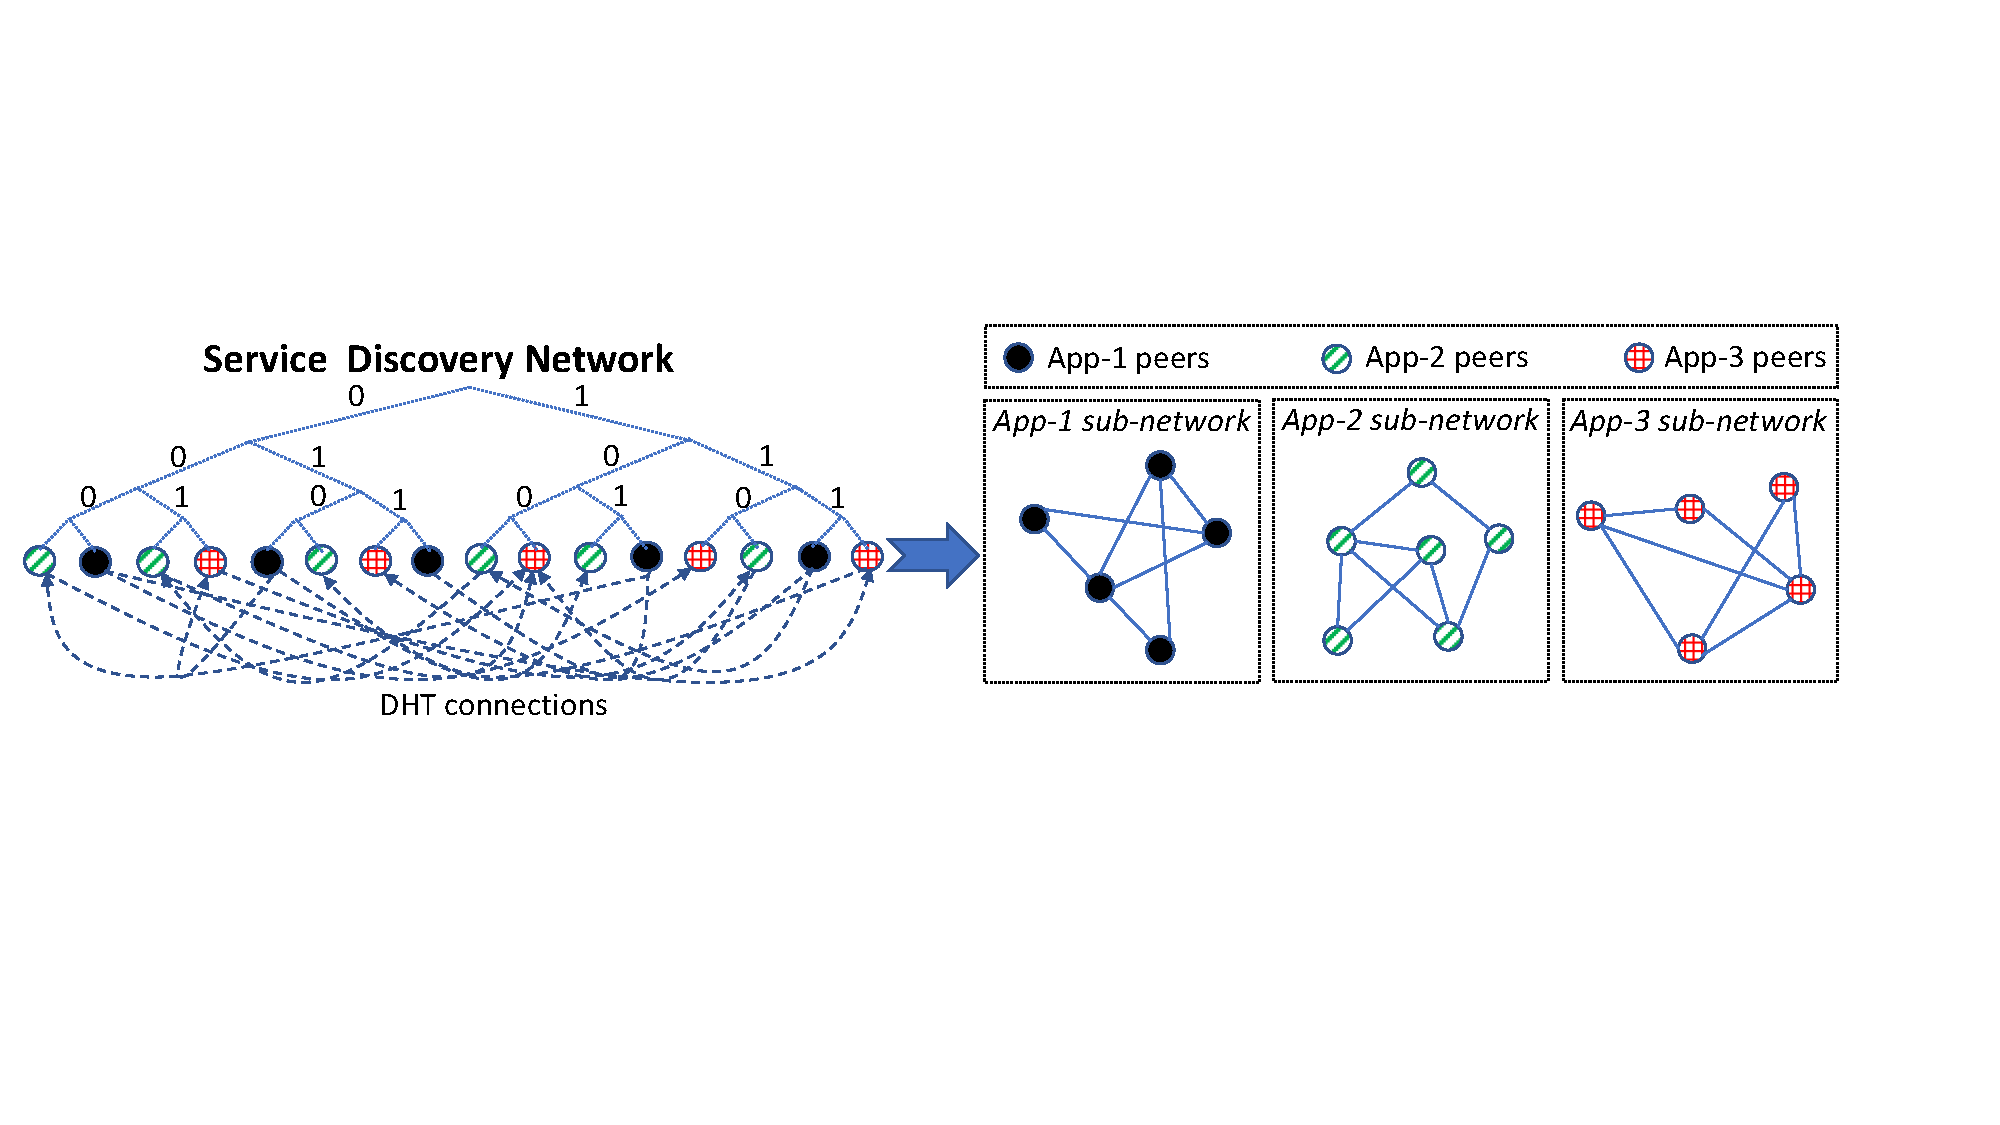
\includegraphics[width=1\linewidth]{img/subnetwork}
    \caption{Formation of application-specific sub-networks using a universal service discovery network.
    }
    \label{fig:subnetwork}
\end{figure}

Service discovery is a particularly sensitive mechanism in the Ethereum platform.
It must ensure that malicious participants to this open network are unable to bias its execution against a victim node or sub-network--and that, despite the ability of these adversaries to operate multiple Sybil identities.
Of particular importance is the protection against \emph{eclipse} attacks, where an adversary would lure its victim(s) into a sub-network formed of only nodes under its control.
Similarly, an adversary may run \emph{denial-of-service} attacks against a specific application, preventing other nodes from discovering peers from the associated sub-network.
On the other hand, the mechanism must remain efficient and scalable.
It is not desirable, in particular, that it relies solely on a fixed set of dedicated registrar nodes maintaining the membership of each application, both for scalability and robustness reasons. Registrar nodes for popular applications could quickly become overwhelmed, and be an easy target for attackers.
In addition, the need to provision dedicated registrar nodes would be a hindrance to the emergence of new applications and (initially) small sub-networks.


The current service discovery mechanism used in the Ethereum platform is part of \discv~\cite{discv4}, a set of protocols leveraging the global DHT.
It employs a simple but robust \emph{random walk} approach.
A node willing to join an application's sub-network simply contacts individually a series of nodes collected from random lookups on the DHT, repeatedly checking application membership until it has collected enough peers participating in this target application.
This approach offers good resilience to malicious behaviors but it suffers from very poor scalability and performance, in particular for small sub-networks.
As more applications join the DHT, the inefficiency of the random discovery process becomes a bottleneck for the entire ecosystem. While alternative solutions for service discovery have been proposed, they are meant for small-scale network~\cite{zhang2002aggregate, helal2002standards}, centralised~\cite{RFC6763}, based on unrealistic assumptions~\cite{danezis2005sybil, danezis2009sybilinfer} or insecure~\cite{baldoni2007tera,scribe,poldercast,banno2015,scribe}. We provide an extensive analysis of these systems in \Cref{sec:related}.

\smallskip
\noindent
\textbf{Contributions.}
%
We detail in this paper \sysname, a novel service discovery mechanism for large-scale, decentralized platforms and its application to Ethereum.
\sysname targets a balance between robustness, i.e., the ability to resist malicious behaviors and Sybil identities, efficiency, i.e., fast service discovery even for small applications, and good load-balance over participating nodes.

After providing background knowledge and reviewing the current service discovery mechanism of Ethereum in \Cref{sec:background}, and detailing our system and thread models in \Cref{sec:model}, we detail \sysname as follows.

In \Cref{sec:placement}, we present how this new protocol enables nodes, members of application sub-networks, to \emph{advertise} their membership to these applications in the form of \emph{service advertisements}.
Any node can act as a \emph{registrar} and store advertisements for any topic.
In contrast with the direct use of the DHT as a key-value store, however, in \sysname service advertisements propagate to a pseudo-random subset of all nodes in the global network.
The density of advertisements for an application increases as a DHT lookup approaches its associated key in the DHT overlay structure.

Robustness, load balancing, and efficiency for the discovery of smaller sub-networks all rely on a novel \emph{admission protocol}, by which registrars accept or reject incoming service advertisements (\Cref{sec:admission}).
It ensures that advertisers cannot effectively flood advertisements at a registrar even when deviating from the protocol or operating Sybils and that less popular topics get a sufficiently high probability to be represented and looked up.

At the core of our novel admission protocol lies the need for registrants to respect a waiting time imposed by the registrars before being able to successfully register their advertisement.
We discuss the design and dynamics of the waiting function in \Cref{sec:waitingTime}.
The function allows limiting the amount of resources used by each node, promotes diversity of topic advertisements stored by each node, and protects against a vast range of malicious behaviors.


We overcome multiple practical challenges, implement \sysname in a simulator as well as in the code base of \emph{discv5}~\cite{discv5} (\ie, Node Discovery protocol version 5) - a new set of P2P protocols replacing \emph{discv4}~\cite{discv4}. 
%We intend to release the full code and dataset of our experiment open source with the unblinded version of this paper.
\hl{Our results show ...}
\sysname already has two full-stack industrial implementations and is scheduled for deployment in the future versions of Ethereum.
%!TEX root = ../main.tex
%=========================================================

\section{Introduction}

%\er{changes:
%\begin{itemize}
%  \item mention there is a DHT but do not say it is Kademlia (in the background mention that it is inspired by Kademlia)
%  \item DHT is not used as-is as a key value store (with a single location for a value) -- change the discussion on this as well (when saying we don't want centralization)
%  \item the registration is done at randomly selected subsets of fixed number of nodes in increasingly-small subsets of peers, drawn from the DHT routing structure (buckets); the likelihood of finding 
%\end{itemize}
%}

With about 23,500 nodes~\cite{discv4-dns-lists}, \oa{this is the number of discoverable nodes, not necessarily the size of the network.} Ethereum is one of the largest decentralized platform currently in operation.
While it is widely known for supporting the blockchain of the same name (also known as the \emph{mainnet}), the Ethereum platform is also home to a number of additional decentralized applications.
This includes blockchains used for test purposes (testnets such as \emph{Ropsted}, \emph{Rinkeby}, or \emph{G\"orli}), divergent blockchains resulting from a past fork (\emph{Ethereum classic}), alternative cryptocurrencies (\emph{Pirl}, \emph{Musicoin}), exchange markets (\emph{Binance}), content delivery networks (\emph{Swarm}), or messaging applications (\emph{Whisper}).
An official Ethereum crawler~\cite{discv4-dns-lists} indicates that the platform already features almost 500 applications, and this number will keep growing in the future.

\begin{figure}[t]
    \includegraphics[width=1\linewidth]{img/ecosystem}
    % \vspace{-2mm}
    \caption{Distribution of the number of nodes in Ethereum's sub-networks, corresponding to different applications.
    Data collected on May 11, 2022.
    Sub-networks are sorted by decreasing popularity.
    A Zipf distribution is given for reference.
    \protect\er{fixme: zipf is Zipf, subnetworks should be sub-networks, there should be a title to the x axis (``Rank'')}
    }
    \label{fig:ecosystem}
\end{figure}

All nodes in the Ethereum platform participate to a \emph{global} peer-to-peer (P2P) network operating a distributed hash table (DHT)~\cite{maymounkov2002kademlia}.
% This global DHT is primarily used for periodic node discovery. % and not as a key-value store (i.e., lookup operations are never used).
% The initial entry in the DHT leverages \emph{bootstrap nodes} operated by the Ethereum foundation, that provide a set of initial contact points, but subsequent maintenance of each nodes' view rely on periodic collection of random peers through DHT lookups. \er{Felix prefers not to discuss this and this is arguably out of scope.}
In addition to joining the global network, every node connects to at least one \emph{sub-network} formed of peers participating to its application(s) of interest. \oa{A node could join more than one sub-networks at a time.}
The size of these sub-networks can vary significantly.
\Cref{fig:ecosystem} depicts the size distribution of Ethereum's main sub-networks.
This distribution features a \emph{long tail}, with a vast majority of applications formed of a few hundred nodes or less, much less than the mainnet or even than any of the testnets.
\mk{We might add some more exciting claims here - "this can become a backbone of the new decentralised Internet/Web3"? From the current description the problem doesn't seem that important.}
In the future, we expect the number of applications to grow significantly, as the Ethereum platform will be selected as the base operation layer by emerging decentralized Internet (web3) projects, amongst other applications.
% Every node in the Ethereum platform participates to a \emph{global} peer-to-peer (P2P) network operating the Kademlia distributed hash table (DHT)~\cite{maymounkov2002kademlia}. \er{how many nodes in this global network?}
% Bootstrapping membership to this general network is handled by a number of trusted \emph{bootstrap nodes} operated by the Ethereum foundation, who provide an initial list of contact peers to nodes entering the network.
% Once joined, every node must connect to one or more sub-network(s) formed of peers participating to its application(s) of interest.
% The size of these sub-networks can vary significantly.
% \Cref{fig:ecosystem} depicts the size distribution of the platform main applications.
% This distribution features a \emph{long tail}, with a vast majority of applications formed of a few thousand nodes or less, much less than the mainnet or even than the testnets. \er{would be useful to give more precise quantiles, e.g., 80\% have less than 1.000 nodes, 90\% less than 200 nodes, etc.}

In this paper, we focus on the \emph{service discovery} mechanism, by which a node participating to the global P2P network discovers an application sub-network.
This mechanism returns a set of peers that are used as entry points to the P2P overlay specific to that application, as illustrated by \Cref{fig:subnetwork}.

\begin{figure}[b!]
    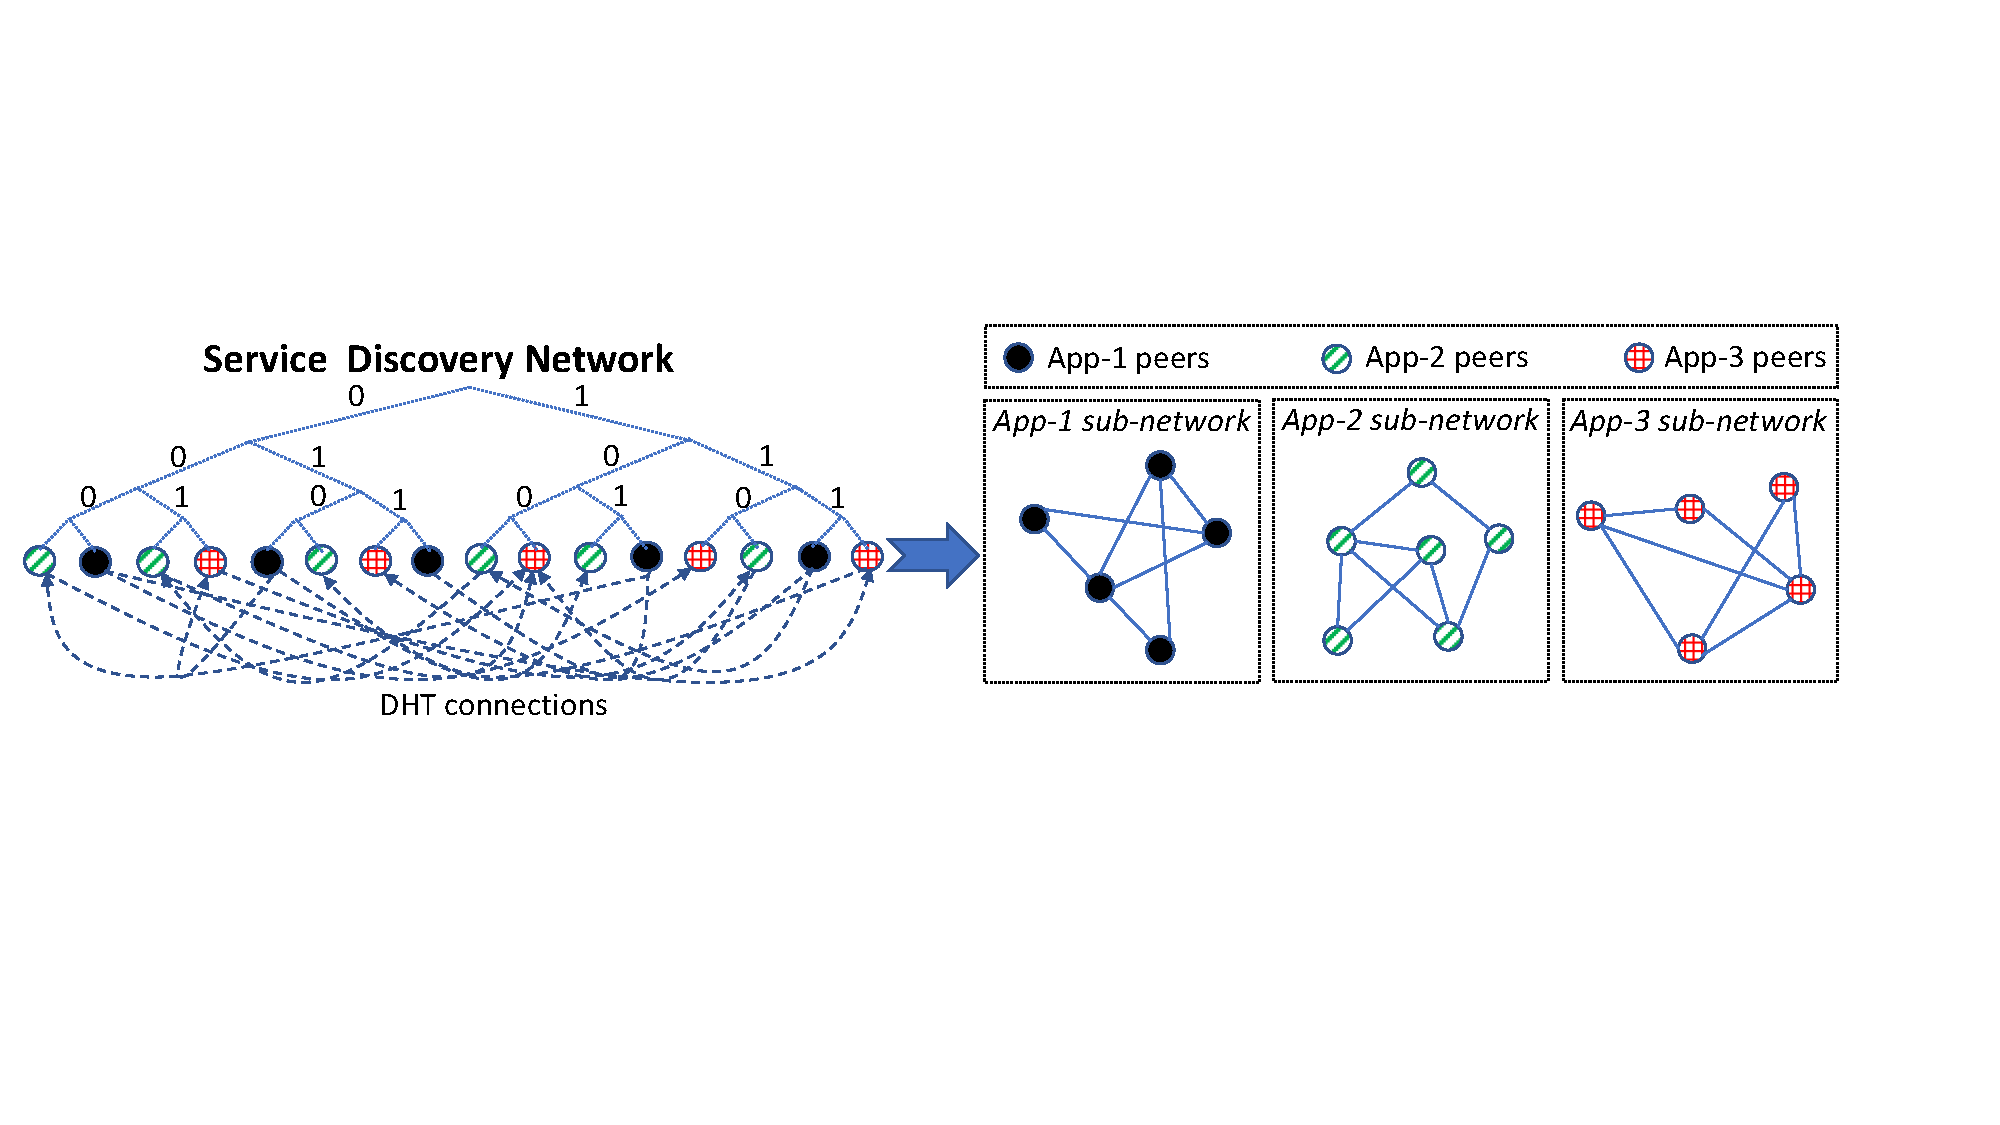
\includegraphics[width=1\linewidth]{img/subnetwork}
    \caption{Formation of application-specific sub-networks using a universal service discovery network.
    % \protect\er{would be good to use different structures for the sub-networks, here they look quite similar}
    }
    \label{fig:subnetwork}
\end{figure}

Service discovery is a particularly sensitive mechanism in the Ethereum platform.
Its implementation must ensure that malicious participants to this open network are unable to bias its execution against a victim node or sub-network--and that, despite the ability of these adversaries to operate multiple Sybil identities.
Of particular importance is the protection against \emph{eclipse} attacks, where an adversary would lure its victim(s) into a sub-network formed of only nodes under its control. %, i.e., by returning only such nodes to a service discovery request.
Similarly, an adversary may run \emph{denial-of-service} attacks against a specific application, preventing other nodes from discovering peers from the associated sub-network.
On the other hand, the mechanism must remain efficient and scalable.
It is not desirable, in particular, that it relies solely on a fixed set of dedicated registrar nodes maintaining the membership of each application, both for scalability and robustness reasons. Registrar nodes for popular applications could quickly become overwhelmed, and be easy target for attackers.
% attackers would have efficient strategies to place Sybils on the path to registrar nodes, or act as such nodes themselves.
In addition, the need to provision dedicated registrar nodes would be a hindrance to the emergence of new applications and (initially) small sub-networks.
% \oa{I would just say that a fixed set of registrar nodes would be an easy target for attackers} \er{fixed}
% \er{also the applications may want to hide themselves (but this clashes completely with our announcement approach)}

The current service discovery mechanism used in the Ethereum platform is part of \discv~\cite{discv4}, a set of protocols leveraging the global DHT.
It employs a simple but robust \emph{random walk} approach.
A node willing to join an application's sub network simply contacts individually a series of nodes collected from random lookups on the DHT, repeatedly checking application membership until it has collected enough peers participating to this target application. % to join the sub-network.
This approach offers good resilience to malicious behaviors
% , and in particular against denial-of-service attacks, 
but it suffers from very poor scalability and performance, in particular for small sub-networks.
As more applications join the DHT, the inefficiency of the random discovery process becomes a bottleneck for the entire ecosystem. \mk{While other alternative solutions for peer sampling have been proposed, they are impractical~\hl{[]}, based on unrealistic assumptions~\hl{[]} or insecure~\hl{[]} and not used in real-life. We provide an extensive analysis of these systems in \Cref{sec:related}.} \er{not sure which papers you want to highlight here specifically?}
% While using the Kademlia DHT as a key/value store to maintain membership information at a specific node or replica group would allow deterministic lookup of this information, regardless of the application's popularity, this solution would suffer from very poor robustness to attacks and would lead to hotspots and overload for nodes in charge of popular services.

\smallskip
\noindent
\textbf{Contributions.}
%
We detail in this paper \sysname, a novel service discovery mechanism for large-scale, decentralized platforms and its application to Ethereum.
\sysname targets a balance between robustness, i.e., the ability to resist malicious behaviors and Sybil identities, efficiency, i.e., fast service discovery even for small applications, and good load-balance over participating nodes.
\sysname is integrated in \emph{discv5}~\cite{discv5} (\ie, Node Discovery protocol version 5) a new set of P2P protocols replacing \emph{discv4} in future versions of Ethereum. \er{ideally add a reference or two here}

After providing background knowledge and reviewing the current service discovery mechanism of Ethereum in \Cref{sec:background}, and detailing our system and thread models in \Cref{sec:model}, we detail \sysname as follows.

In \Cref{sec:placement}, we present how this new protocol enables nodes, members of application sub-networks, to \emph{advertise} their membership to these applications in the form of \emph{service advertisements}.
Any node can act as a \emph{registrar} and store advertisements for any topic.
In contrast with a direct use of the DHT as a key-value store, however, in \sysname service advertisements propagate to a pseudo-random subset of all nodes in the global network.
The density of advertisements for an application increases as a DHT lookup approaches its associated key in the DHT overlay structure.\mk{We don't cover lookup. The description may be also downplaying the contribution.}\er{I am not sure to understand this comment, might need to discuss it.}
% As such, \sysname enables efficient lookup of advertisements for any given service.

Robustness, load balancing, and efficiency for the discovery of smaller sub-networks all rely on a novel \emph{admission protocol}, by which registrars accept or reject incoming service advertisements.
This mechanism is detailed in \Cref{sec:registration}.
It ensures that advertisers cannot effectively flood advertisements at a registrar even when deviating from the protocol or operating Sybils, and that less popular topics get sufficiently high probability to be represented and looked up. \er{not sure about this sentence, we do not provide any bound, this is all probabilistic.} \er{I did not keep the comment about the intermediary state as I am not sure what it is about.}

At the core our novel admission protocol lies the need for registrants to respect a waiting time imposed by the registrars before being able to successfully register their advertisement.
We discuss the design and dynamics of the waiting function in \Cref{sec:waitingTime}.
The function allows limiting the amount of resources used by each node, promotes diversity of topic advertisements stored by each node, and protects against a vast range of malicious behaviors.

We implemented \sysname in a simulator as well as in the code base of \emph{discv5}. \michal{Mentioned it's schedule to be included in discv5.}
We intend to release the full code and dataset of our experiment open source with the unblinded version of this paper.
Our results show ...



%%!TEX root = ../main.tex
%=========================================================

%Background
% -> I would present Kademlia directly rather than a generic DHT model (which we can assume is common knowledge for the readers) -- we only want to summarize what operations it supports and directly explain how Kademlia implements it.
% -> The DHT description is both very general (concepts without explaining the graph structures) and very specific (names of the messages exchanged between the nodes).%!TEX root = ../main.tex
%=========================================================

%Background
% -> I would present Kademlia directly rather than a generic DHT model (which we can assume is common knowledge for the readers) -- we only want to summarize what operations it supports and directly explain how Kademlia implements it.
% -> The DHT description is both very general (concepts without explaining the graph structures) and very specific (names of the messages exchanged between the nodes).%!TEX root = ../main.tex
%=========================================================

%Background
% -> I would present Kademlia directly rather than a generic DHT model (which we can assume is common knowledge for the readers) -- we only want to summarize what operations it supports and directly explain how Kademlia implements it.
% -> The DHT description is both very general (concepts without explaining the graph structures) and very specific (names of the messages exchanged between the nodes).\include{sections/new_background.tex}
% -> 2.2 why present the Ethereum network as similar to a DHT but not writing it is one? This is confusing imho
% -> What is a subprotocol in the context of 2.2?
% -> It seems to me that this background section should be remodeled into a problem statement that focuses on how Ethereum does service discovery and identifies clearly the issues with scalability and attacks.

\section{Background}
\label{sec:background}

We start by detailing the operation of the Ethereum's global DHT, which is an evolution of the canonical Kademlia~\cite{maymounkov2002kademlia} DHT.
Then, we present the current service discovery mechanism, part of Ethereum's \emph{discv4} series of protocol operating atop this DHT, and discuss its shortcomings.

\subsection{The Ethereum global DHT}
\label{sec:background:dht}

All nodes in Ethereum participate to a global distributed hash table (DHT).
A DHT is a structured overlay network allowing lookup operations, i.e., locating a node or group of nodes in charge of a particular \emph{key} in a target \emph{key space}~\cite{chord,rowstron2001pastry}. Ethereum uses an evolution of Kademlia~\cite{maymounkov2002kademlia}, a robust and mature DHT design. % as its global DHT.
Every node in the overlay is assigned a unique identifier (\emph{node ID}), drawn from the same key space as items, i.e., information stored in the DHT. %\mk{we haven't mention item storage before}
Ethereum DHT assigns a specific key $i$ to the node that is the \emph{closest} to $i$ in that space.
This distance $d$ between two keys $x$ and $y$ is a logarithm of their bitwise exclusive or (XOR) interpreted as an integer, \ie, $d(x,y) = \textit{log}_2(x \oplus y)$ (\ie the length of differing suffix in bits).

Each node $N$ in the overlay maintains a \emph{routing table} storing a set of peers, each with its \emph{node ID} and reachability information, \ie, IP address and port numbers.
The routing table is partitioned into $m$ \textit{buckets}, numbered zero through $m-1$, where $m$ is a global system parameter.
Bucket $i$ contains a list of up to $k$ peers, whose IDs share a common prefix of length $i$ with $N$.
% The last bucket (\ie, bucket $m-1$) additionally contains peers whose IDs share a prefix of length exceeding $m-1$ bits with the local node. \er{I do not see the point/interest of this precision, this is already covered by the previous sentence.}

% A newly instantiated DHT node typically populates its routing table with a set of (hard-coded) bootstrap nodes\footnote{While other approaches where proposed based on social relations between nodes, currently, most of the deployed DHTs use the bootstrap node approach.}.

\begin{figure}
    \includegraphics[width=0.4\textwidth]{img/kademlia}
    \caption{Organization of the DHT routing table.}
    \label{fig:kademlia}
 \end{figure}

\smallskip
\noindent
\textbf{Lookups.}
%
The bucket partitioning scheme divides the key space from the point of view of $N$ into disjoint intervals, halving in length every time the bucket's associated prefix includes one more common bit with $N$'s ID.
As a result, a node's routing table provides a more detailed (\ie, fine grained) view of the subset of the network with closer node IDs and a less detailed view of nodes with distant IDs.
This property is essential for efficiency and enables lookup operations that take a logarithmic number of steps (\emph{hops}) in the number of nodes in the network.
It allows, in addition, a degree of flexibility as each bucket can contain \textit{any} peer sampled from those whose IDs fall within the corresponding interval of key space.

Lookups rely on a number $\alpha$ of concurrent routing operations (or \emph{walks}) towards the target key.
In the original Kademlia~\cite{maymounkov2002kademlia}, these lookups specify the target key, and collect from each node in the process the $k$ closest nodes to that target, which are fed into the querying node's own routing table.
The process stops when up to $k$ nodes closest to the target are found. \er{seems contradictory when the goal is to find the exact one that is the closest?}
The Ethereum DHT 
\er{stopped here, not sure what level of detail we need to the new dht lookup of ethereum dht we need.}
In Kademlia, the lookup procedure for a target key involves $\alpha$ ``walks'', each searching for the target in parallel. During each walk, the initiator node iteratively selects the closest peer to the target from its routing table and sends the peer a FIND\_NODE query message, specifying the target key. A peer responds to a FIND\_NODE message by returning information on up to $k$ closest nodes (\ie ID, IP, and port) to the given target from its routing table. The initiator node then adds the returned peers to its routing table and iteratively sends another FIND\_NODE message to the closest known peer, extending the traversed path by the walk, until the process converges to a stable $k$ closest known peers to the target.

\er{need to simplify the following and make it a single paragraph as part of the lookup paragraph}

Ethereum's DHT implementation uses a rather ``crude'' distance metric allowing nodes to hide their target from other peers in the lookups. Specifically, the distance of a key to a node is the common prefix length of the key and the node's ID, which corresponds to the bucket number of the key where the node would insert the key, following the same bucket partitioning scheme with vanilla Kademlia.

A key difference in Ethereum's parallel lookup process (\ie $\alpha$ walks) is that the initiating nodes specify the distance of an undisclosed target in their FIND\_NODE messages rather than the target key itself. Each peer responds to a FIND\_NODE message by returning up to $k$ peers from its bucket whose number corresponds to the supplied distance in the message. In case, there are less than $k$ peers in its bucket, a node can return peers from adjacent buckets. The initiating node terminates the lookup when the process converges to a stable set of (not necessarily $k$) closest nodes based on the modified distance metric, \ie no new peers in the target key's bucket.

\oa{briefly mention and reference the eclipsing counter-measures of Ethereum DHT since our protocol assumes the DHT is secure}

\subsection{\emph{discv4} service discovery}
\label{sec:background:discv4}
In the current service discovery protocol, DISCV4RANDOM, a node performs \textit{random walks} through the DHT and establishes connections to encountered peers after verifying the supported protocols of the peers at the application level. In a random walk, a node picks a random target key and performs a lookup towards the distance corresponding to the target following the parallel search process explained above. Each node maintains a \textit{discovery table} whose sole purpose is to store a set of peers that the node has come across during its parallel random walks.\mk{The discovery table seems like a implementation detail. Maybe just say that we initiate handshakes with encountered/returned peers?} %This table serves as a basis for establishing sub-protocol connections as we describe below.  

%\dk{could mention DNS discovery\footnote{https://eips.ethereum.org/EIPS/eip-1459} as a means for discv5 bootstrap. We implemented this for Waku v2.}

A node starts establishing application-level sessions (\ie handshake) with the peers in its discovery table in order to identify their applications, \ie the sub-network(s) they are part of. A handshake involves a secure channel establishment between the initiator node and its discovered peer and therefore incurs some overhead to both endpoints. When the node discovers during the handshake that the discovered peer is part of a target application, the initiator node can follow up with a connection request to the peer to establish an application-level connection. The objective of a node is to fill up a number of \textit{application-level connection slots} with outbound (\ie initiated by the node) connections. The process of node discovery is suspended when a node has filled up all outbound slots. Nodes also reserve a number of inbound connection slots that can be filled with connections initiated by other nodes. 

\subsection{Security and Efficiency of DISCV4RANDOM}
\label{sec:securityEfficiency}
\mk{The below is too long. I also don't think it's a good place to discuss in more details potential attacks.}
In the context of blockchains and cryptocurrency, security is a key requirement for a service discovery protocol. A potential attack on any peer discovery protocol is the eclipse attack, where an adversary monopolises all the connections of a victim node with its Sybils, effectively separating the victim from the rest of the network. In blockchain systems, eclipse attacks are typically a pre-cursor to financially-motivated attacks such as double spending and stubborn mining~\cite{henningsen2019eclipsing}.

Because eclipsing can apply to any peer discovery process, it concerns both the DHT-level (\ie Kademlia routing table) and application-level peer selection. Peer selection through random sampling, as used in Kademlia and DISCV4RANDOM, is reasonably resilient against eclipse attacks, because attackers can not strategically place their Sybil identities in the keyspace to increase their chance of being discovered by victims, \ie all locations in the keyspace have equal chance of being discovered.

\felix{This is not completely true and we need to find a better reasoning here. It is technically feasible to generate chosed IDs because mining hardware exists for keccak256.}

%At the same time, the buckets of the routing table are well protected from eclipsing owing to the flexible (random) peer selection mechanism inherited from Kademlia (Section~\ref{sec:kademlia}). Random peer selection is effective because attackers can not strategically place their Sybil identities in the keyspace to increase their chance of being discovered by victims, \ie all locations in the keyspace have equal chance of being discovered.

On the other hand, the brute-force approach of expensive handshakes with randomly encountered nodes has several drawbacks in terms of efficiency. First of all, handshakes with peers not in the target sub-network are wasteful and incur unnecessary overhead. More importantly, it can take very long to discover peers that are part of an unpopular sub-network (\ie an application for which there is only a small number of peers). %\Cref{tab:discv4Overhead} provides the average number of wasteful handshakes until one peer is found for the target application, given the application's popularity, \ie adoption by the percentage of nodes in the network\footnote{Appendix contains the details of the calculations}. %
For applications with low popularity, the number of handshakes can be excessive, \ie on the order of thousands when 0.1\% of the nodes are running the target application. Because all the applications are initially unpopular, the upfront cost of building a sub-network can be large and finding peers can take long time.

%\dk{A math. estimation would be nice here.}

%\begin{table} [!hbt]
%\caption{Average number of wasteful handshakes until one successful peer discovery for a given popularity of the target application }
%\label{tab:discv4Overhead}
%\renewcommand{\arraystretch}{1.5}
%\renewcommand{\tabcolsep}{0.5em}
%\centering
%\scriptsize{
%\begin{tabular} {c|c}
%\textbf{Popularity (in \% of population)} & \textbf{Number of Handshakes} \\
%\hline
%0.01 & 6944 \\ 
%\hline
%0.05 & 1392 \\
%\hline
%0.1 & 704 \\
%\hline
%1 & 64 \\
%\bottomrule
%\end{tabular}
%}
%\vspace{-0.2in}
%\end{table}

% -> 2.2 why present the Ethereum network as similar to a DHT but not writing it is one? This is confusing imho
% -> What is a subprotocol in the context of 2.2?
% -> It seems to me that this background section should be remodeled into a problem statement that focuses on how Ethereum does service discovery and identifies clearly the issues with scalability and attacks.

\section{Background}
\label{sec:background}

We start by detailing the operation of the Ethereum's global DHT, which is an evolution of the canonical Kademlia~\cite{maymounkov2002kademlia} DHT.
Then, we present the current service discovery mechanism, part of Ethereum's \emph{discv4} series of protocol operating atop this DHT, and discuss its shortcomings.

\subsection{The Ethereum global DHT}
\label{sec:background:dht}

All nodes in Ethereum participate to a global distributed hash table (DHT).
A DHT is a structured overlay network allowing lookup operations, i.e., locating a node or group of nodes in charge of a particular \emph{key} in a target \emph{key space}~\cite{chord,rowstron2001pastry}. Ethereum uses an evolution of Kademlia~\cite{maymounkov2002kademlia}, a robust and mature DHT design. % as its global DHT.
Every node in the overlay is assigned a unique identifier (\emph{node ID}), drawn from the same key space as items, i.e., information stored in the DHT. %\mk{we haven't mention item storage before}
Ethereum DHT assigns a specific key $i$ to the node that is the \emph{closest} to $i$ in that space.
This distance $d$ between two keys $x$ and $y$ is a logarithm of their bitwise exclusive or (XOR) interpreted as an integer, \ie, $d(x,y) = \textit{log}_2(x \oplus y)$ (\ie the length of differing suffix in bits).

Each node $N$ in the overlay maintains a \emph{routing table} storing a set of peers, each with its \emph{node ID} and reachability information, \ie, IP address and port numbers.
The routing table is partitioned into $m$ \textit{buckets}, numbered zero through $m-1$, where $m$ is a global system parameter.
Bucket $i$ contains a list of up to $k$ peers, whose IDs share a common prefix of length $i$ with $N$.
% The last bucket (\ie, bucket $m-1$) additionally contains peers whose IDs share a prefix of length exceeding $m-1$ bits with the local node. \er{I do not see the point/interest of this precision, this is already covered by the previous sentence.}

% A newly instantiated DHT node typically populates its routing table with a set of (hard-coded) bootstrap nodes\footnote{While other approaches where proposed based on social relations between nodes, currently, most of the deployed DHTs use the bootstrap node approach.}.

\begin{figure}
    \includegraphics[width=0.4\textwidth]{img/kademlia}
    \caption{Organization of the DHT routing table.}
    \label{fig:kademlia}
 \end{figure}

\smallskip
\noindent
\textbf{Lookups.}
%
The bucket partitioning scheme divides the key space from the point of view of $N$ into disjoint intervals, halving in length every time the bucket's associated prefix includes one more common bit with $N$'s ID.
As a result, a node's routing table provides a more detailed (\ie, fine grained) view of the subset of the network with closer node IDs and a less detailed view of nodes with distant IDs.
This property is essential for efficiency and enables lookup operations that take a logarithmic number of steps (\emph{hops}) in the number of nodes in the network.
It allows, in addition, a degree of flexibility as each bucket can contain \textit{any} peer sampled from those whose IDs fall within the corresponding interval of key space.

Lookups rely on a number $\alpha$ of concurrent routing operations (or \emph{walks}) towards the target key.
In the original Kademlia~\cite{maymounkov2002kademlia}, these lookups specify the target key, and collect from each node in the process the $k$ closest nodes to that target, which are fed into the querying node's own routing table.
The process stops when up to $k$ nodes closest to the target are found. \er{seems contradictory when the goal is to find the exact one that is the closest?}
The Ethereum DHT 
\er{stopped here, not sure what level of detail we need to the new dht lookup of ethereum dht we need.}
In Kademlia, the lookup procedure for a target key involves $\alpha$ ``walks'', each searching for the target in parallel. During each walk, the initiator node iteratively selects the closest peer to the target from its routing table and sends the peer a FIND\_NODE query message, specifying the target key. A peer responds to a FIND\_NODE message by returning information on up to $k$ closest nodes (\ie ID, IP, and port) to the given target from its routing table. The initiator node then adds the returned peers to its routing table and iteratively sends another FIND\_NODE message to the closest known peer, extending the traversed path by the walk, until the process converges to a stable $k$ closest known peers to the target.

\er{need to simplify the following and make it a single paragraph as part of the lookup paragraph}

Ethereum's DHT implementation uses a rather ``crude'' distance metric allowing nodes to hide their target from other peers in the lookups. Specifically, the distance of a key to a node is the common prefix length of the key and the node's ID, which corresponds to the bucket number of the key where the node would insert the key, following the same bucket partitioning scheme with vanilla Kademlia.

A key difference in Ethereum's parallel lookup process (\ie $\alpha$ walks) is that the initiating nodes specify the distance of an undisclosed target in their FIND\_NODE messages rather than the target key itself. Each peer responds to a FIND\_NODE message by returning up to $k$ peers from its bucket whose number corresponds to the supplied distance in the message. In case, there are less than $k$ peers in its bucket, a node can return peers from adjacent buckets. The initiating node terminates the lookup when the process converges to a stable set of (not necessarily $k$) closest nodes based on the modified distance metric, \ie no new peers in the target key's bucket.

\oa{briefly mention and reference the eclipsing counter-measures of Ethereum DHT since our protocol assumes the DHT is secure}

\subsection{\emph{discv4} service discovery}
\label{sec:background:discv4}
In the current service discovery protocol, DISCV4RANDOM, a node performs \textit{random walks} through the DHT and establishes connections to encountered peers after verifying the supported protocols of the peers at the application level. In a random walk, a node picks a random target key and performs a lookup towards the distance corresponding to the target following the parallel search process explained above. Each node maintains a \textit{discovery table} whose sole purpose is to store a set of peers that the node has come across during its parallel random walks.\mk{The discovery table seems like a implementation detail. Maybe just say that we initiate handshakes with encountered/returned peers?} %This table serves as a basis for establishing sub-protocol connections as we describe below.  

%\dk{could mention DNS discovery\footnote{https://eips.ethereum.org/EIPS/eip-1459} as a means for discv5 bootstrap. We implemented this for Waku v2.}

A node starts establishing application-level sessions (\ie handshake) with the peers in its discovery table in order to identify their applications, \ie the sub-network(s) they are part of. A handshake involves a secure channel establishment between the initiator node and its discovered peer and therefore incurs some overhead to both endpoints. When the node discovers during the handshake that the discovered peer is part of a target application, the initiator node can follow up with a connection request to the peer to establish an application-level connection. The objective of a node is to fill up a number of \textit{application-level connection slots} with outbound (\ie initiated by the node) connections. The process of node discovery is suspended when a node has filled up all outbound slots. Nodes also reserve a number of inbound connection slots that can be filled with connections initiated by other nodes. 

\subsection{Security and Efficiency of DISCV4RANDOM}
\label{sec:securityEfficiency}
\mk{The below is too long. I also don't think it's a good place to discuss in more details potential attacks.}
In the context of blockchains and cryptocurrency, security is a key requirement for a service discovery protocol. A potential attack on any peer discovery protocol is the eclipse attack, where an adversary monopolises all the connections of a victim node with its Sybils, effectively separating the victim from the rest of the network. In blockchain systems, eclipse attacks are typically a pre-cursor to financially-motivated attacks such as double spending and stubborn mining~\cite{henningsen2019eclipsing}.

Because eclipsing can apply to any peer discovery process, it concerns both the DHT-level (\ie Kademlia routing table) and application-level peer selection. Peer selection through random sampling, as used in Kademlia and DISCV4RANDOM, is reasonably resilient against eclipse attacks, because attackers can not strategically place their Sybil identities in the keyspace to increase their chance of being discovered by victims, \ie all locations in the keyspace have equal chance of being discovered.

\felix{This is not completely true and we need to find a better reasoning here. It is technically feasible to generate chosed IDs because mining hardware exists for keccak256.}

%At the same time, the buckets of the routing table are well protected from eclipsing owing to the flexible (random) peer selection mechanism inherited from Kademlia (Section~\ref{sec:kademlia}). Random peer selection is effective because attackers can not strategically place their Sybil identities in the keyspace to increase their chance of being discovered by victims, \ie all locations in the keyspace have equal chance of being discovered.

On the other hand, the brute-force approach of expensive handshakes with randomly encountered nodes has several drawbacks in terms of efficiency. First of all, handshakes with peers not in the target sub-network are wasteful and incur unnecessary overhead. More importantly, it can take very long to discover peers that are part of an unpopular sub-network (\ie an application for which there is only a small number of peers). %\Cref{tab:discv4Overhead} provides the average number of wasteful handshakes until one peer is found for the target application, given the application's popularity, \ie adoption by the percentage of nodes in the network\footnote{Appendix contains the details of the calculations}. %
For applications with low popularity, the number of handshakes can be excessive, \ie on the order of thousands when 0.1\% of the nodes are running the target application. Because all the applications are initially unpopular, the upfront cost of building a sub-network can be large and finding peers can take long time.

%\dk{A math. estimation would be nice here.}

%\begin{table} [!hbt]
%\caption{Average number of wasteful handshakes until one successful peer discovery for a given popularity of the target application }
%\label{tab:discv4Overhead}
%\renewcommand{\arraystretch}{1.5}
%\renewcommand{\tabcolsep}{0.5em}
%\centering
%\scriptsize{
%\begin{tabular} {c|c}
%\textbf{Popularity (in \% of population)} & \textbf{Number of Handshakes} \\
%\hline
%0.01 & 6944 \\ 
%\hline
%0.05 & 1392 \\
%\hline
%0.1 & 704 \\
%\hline
%1 & 64 \\
%\bottomrule
%\end{tabular}
%}
%\vspace{-0.2in}
%\end{table}

% -> 2.2 why present the Ethereum network as similar to a DHT but not writing it is one? This is confusing imho
% -> What is a subprotocol in the context of 2.2?
% -> It seems to me that this background section should be remodeled into a problem statement that focuses on how Ethereum does service discovery and identifies clearly the issues with scalability and attacks.

\section{Background}
\label{sec:background}

We start by detailing the operation of the Ethereum's global DHT, which is an evolution of the canonical Kademlia~\cite{maymounkov2002kademlia} DHT.
Then, we present the current service discovery mechanism, part of Ethereum's \emph{discv4} series of protocol operating atop this DHT, and discuss its shortcomings.

\subsection{The Ethereum global DHT}
\label{sec:background:dht}

All nodes in Ethereum participate to a global distributed hash table (DHT).
A DHT is a structured overlay network allowing lookup operations, i.e., locating a node or group of nodes in charge of a particular \emph{key} in a target \emph{key space}~\cite{chord,rowstron2001pastry}. Ethereum uses an evolution of Kademlia~\cite{maymounkov2002kademlia}, a robust and mature DHT design. % as its global DHT.
Every node in the overlay is assigned a unique identifier (\emph{node ID}), drawn from the same key space as items, i.e., information stored in the DHT. %\mk{we haven't mention item storage before}
Ethereum DHT assigns a specific key $i$ to the node that is the \emph{closest} to $i$ in that space.
This distance $d$ between two keys $x$ and $y$ is a logarithm of their bitwise exclusive or (XOR) interpreted as an integer, \ie, $d(x,y) = \textit{log}_2(x \oplus y)$ (\ie the length of differing suffix in bits).

Each node $N$ in the overlay maintains a \emph{routing table} storing a set of peers, each with its \emph{node ID} and reachability information, \ie, IP address and port numbers.
The routing table is partitioned into $m$ \textit{buckets}, numbered zero through $m-1$, where $m$ is a global system parameter.
Bucket $i$ contains a list of up to $k$ peers, whose IDs share a common prefix of length $i$ with $N$.
% The last bucket (\ie, bucket $m-1$) additionally contains peers whose IDs share a prefix of length exceeding $m-1$ bits with the local node. \er{I do not see the point/interest of this precision, this is already covered by the previous sentence.}

% A newly instantiated DHT node typically populates its routing table with a set of (hard-coded) bootstrap nodes\footnote{While other approaches where proposed based on social relations between nodes, currently, most of the deployed DHTs use the bootstrap node approach.}.

\begin{figure}
    \includegraphics[width=0.4\textwidth]{img/kademlia}
    \caption{Organization of the DHT routing table.\mk{Do we need this figure?}}
    \label{fig:kademlia}
 \end{figure}

\smallskip
\noindent
\textbf{Lookups.}
%
The bucket partitioning scheme divides the key space from the point of view of $N$ into disjoint intervals, halving in length every time the bucket's associated prefix includes one more common bit with $N$'s ID.
As a result, a node's routing table provides a more detailed (\ie, fine grained) view of the subset of the network with closer node IDs and a less detailed view of nodes with distant IDs.
This property is essential for efficiency and enables lookup operations that take a logarithmic number of steps (\emph{hops}) in the number of nodes in the network.
It allows, in addition, a degree of flexibility as each bucket can contain \textit{any} peer sampled from those whose IDs fall within the corresponding interval of key space.

Lookups rely on a number $\alpha$ of concurrent routing operations (or \emph{walks}) towards the target key.
In the original Kademlia~\cite{maymounkov2002kademlia}, these lookups specify the target key, and collect from each node in the process the $k$ closest nodes to that target, which are fed into the querying node's own routing table.
The process stops when up to $k$ nodes closest to the target are found. \er{seems contradictory when the goal is to find the exact one that is the closest?}
The Ethereum DHT 
\er{stopped here, not sure what level of detail we need to the new dht lookup of ethereum dht we need.}
In Kademlia, the lookup procedure for a target key involves $\alpha$ ``walks'', each searching for the target in parallel. During each walk, the initiator node iteratively selects the closest peer to the target from its routing table and sends the peer a FIND\_NODE query message, specifying the target key. A peer responds to a FIND\_NODE message by returning information on up to $k$ closest nodes (\ie ID, IP, and port) to the given target from its routing table. The initiator node then adds the returned peers to its routing table and iteratively sends another FIND\_NODE message to the closest known peer, extending the traversed path by the walk, until the process converges to a stable $k$ closest known peers to the target.

\er{need to simplify the following and make it a single paragraph as part of the lookup paragraph}

Ethereum's DHT implementation uses a rather ``crude'' distance metric allowing nodes to hide their target from other peers in the lookups. Specifically, the distance of a key to a node is the common prefix length of the key and the node's ID, which corresponds to the bucket number of the key where the node would insert the key, following the same bucket partitioning scheme with vanilla Kademlia.

A key difference in Ethereum's parallel lookup process (\ie $\alpha$ walks) is that the initiating nodes specify the distance of an undisclosed target in their FIND\_NODE messages rather than the target key itself. Each peer responds to a FIND\_NODE message by returning up to $k$ peers from its bucket whose number corresponds to the supplied distance in the message. In case, there are less than $k$ peers in its bucket, a node can return peers from adjacent buckets. The initiating node terminates the lookup when the process converges to a stable set of (not necessarily $k$) closest nodes based on the modified distance metric, \ie no new peers in the target key's bucket.

\oa{briefly mention and reference the eclipsing counter-measures of Ethereum DHT since our protocol assumes the DHT is secure}

\subsection{\emph{discv4} service discovery}
\label{sec:background:discv4}
In the current service discovery protocol, DISCV4RANDOM, a node performs \textit{random walks} through the DHT and establishes connections to encountered peers after verifying the supported protocols of the peers at the application level. In a random walk, a node picks a random target key and performs a lookup towards the distance corresponding to the target following the parallel search process explained above. Each node maintains a \textit{discovery table} whose sole purpose is to store a set of peers that the node has come across during its parallel random walks.\mk{The discovery table seems like a implementation detail. Maybe just say that we initiate handshakes with encountered/returned peers?} %This table serves as a basis for establishing sub-protocol connections as we describe below.  

%\dk{could mention DNS discovery\footnote{https://eips.ethereum.org/EIPS/eip-1459} as a means for discv5 bootstrap. We implemented this for Waku v2.}

A node starts establishing application-level sessions (\ie handshake) with the peers in its discovery table in order to identify their applications, \ie the sub-network(s) they are part of. A handshake involves a secure channel establishment between the initiator node and its discovered peer and therefore incurs some overhead to both endpoints. When the node discovers during the handshake that the discovered peer is part of a target application, the initiator node can follow up with a connection request to the peer to establish an application-level connection. The objective of a node is to fill up a number of \textit{application-level connection slots} with outbound (\ie initiated by the node) connections. The process of node discovery is suspended when a node has filled up all outbound slots. Nodes also reserve a number of inbound connection slots that can be filled with connections initiated by other nodes. 

\subsection{Security and Efficiency of DISCV4RANDOM}
\label{sec:securityEfficiency}
\mk{The below is too long. I also don't think it's a good place to discuss in more details potential attacks.}
In the context of blockchains and cryptocurrency, security is a key requirement for a service discovery protocol. A potential attack on any peer discovery protocol is the eclipse attack, where an adversary monopolises all the connections of a victim node with its Sybils, effectively separating the victim from the rest of the network. In blockchain systems, eclipse attacks are typically a pre-cursor to financially-motivated attacks such as double spending and stubborn mining~\cite{henningsen2019eclipsing}.

Because eclipsing can apply to any peer discovery process, it concerns both the DHT-level (\ie Kademlia routing table) and application-level peer selection. Peer selection through random sampling, as used in Kademlia and DISCV4RANDOM, is reasonably resilient against eclipse attacks, because attackers can not strategically place their Sybil identities in the keyspace to increase their chance of being discovered by victims, \ie all locations in the keyspace have equal chance of being discovered.

\felix{This is not completely true and we need to find a better reasoning here. It is technically feasible to generate chosed IDs because mining hardware exists for keccak256.}

%At the same time, the buckets of the routing table are well protected from eclipsing owing to the flexible (random) peer selection mechanism inherited from Kademlia (Section~\ref{sec:kademlia}). Random peer selection is effective because attackers can not strategically place their Sybil identities in the keyspace to increase their chance of being discovered by victims, \ie all locations in the keyspace have equal chance of being discovered.

On the other hand, the brute-force approach of expensive handshakes with randomly encountered nodes has several drawbacks in terms of efficiency. First of all, handshakes with peers not in the target sub-network are wasteful and incur unnecessary overhead. More importantly, it can take very long to discover peers that are part of an unpopular sub-network (\ie an application for which there is only a small number of peers). %\Cref{tab:discv4Overhead} provides the average number of wasteful handshakes until one peer is found for the target application, given the application's popularity, \ie adoption by the percentage of nodes in the network\footnote{Appendix contains the details of the calculations}. %
For applications with low popularity, the number of handshakes can be excessive, \ie on the order of thousands when 0.1\% of the nodes are running the target application. Because all the applications are initially unpopular, the upfront cost of building a sub-network can be large and finding peers can take long time.

%\dk{A math. estimation would be nice here.}

%\begin{table} [!hbt]
%\caption{Average number of wasteful handshakes until one successful peer discovery for a given popularity of the target application }
%\label{tab:discv4Overhead}
%\renewcommand{\arraystretch}{1.5}
%\renewcommand{\tabcolsep}{0.5em}
%\centering
%\scriptsize{
%\begin{tabular} {c|c}
%\textbf{Popularity (in \% of population)} & \textbf{Number of Handshakes} \\
%\hline
%0.01 & 6944 \\ 
%\hline
%0.05 & 1392 \\
%\hline
%0.1 & 704 \\
%\hline
%1 & 64 \\
%\bottomrule
%\end{tabular}
%}
%\vspace{-0.2in}
%\end{table}

%\input{sections/background_high_level}
%!TEX root = ../main.tex
%=========================================================

%Background
% -> I would present Kademlia directly rather than a generic DHT model (which we can assume is common knowledge for the readers) -- we only want to summarize what operations it supports and directly explain how Kademlia implements it.
% -> The DHT description is both very general (concepts without explaining the graph structures) and very specific (names of the messages exchanged between the nodes).%!TEX root = ../main.tex
%=========================================================

%Background
% -> I would present Kademlia directly rather than a generic DHT model (which we can assume is common knowledge for the readers) -- we only want to summarize what operations it supports and directly explain how Kademlia implements it.
% -> The DHT description is both very general (concepts without explaining the graph structures) and very specific (names of the messages exchanged between the nodes).%!TEX root = ../main.tex
%=========================================================

%Background
% -> I would present Kademlia directly rather than a generic DHT model (which we can assume is common knowledge for the readers) -- we only want to summarize what operations it supports and directly explain how Kademlia implements it.
% -> The DHT description is both very general (concepts without explaining the graph structures) and very specific (names of the messages exchanged between the nodes).\include{sections/new_background.tex}
% -> 2.2 why present the Ethereum network as similar to a DHT but not writing it is one? This is confusing imho
% -> What is a subprotocol in the context of 2.2?
% -> It seems to me that this background section should be remodeled into a problem statement that focuses on how Ethereum does service discovery and identifies clearly the issues with scalability and attacks.

\section{Background}
\label{sec:background}

We start by detailing the operation of the Ethereum's global DHT, which is an evolution of the canonical Kademlia~\cite{maymounkov2002kademlia} DHT.
Then, we present the current service discovery mechanism, part of Ethereum's \emph{discv4} series of protocol operating atop this DHT, and discuss its shortcomings.

\subsection{The Ethereum global DHT}
\label{sec:background:dht}

All nodes in Ethereum participate to a global distributed hash table (DHT).
A DHT is a structured overlay network allowing lookup operations, i.e., locating a node or group of nodes in charge of a particular \emph{key} in a target \emph{key space}~\cite{chord,rowstron2001pastry}. Ethereum uses an evolution of Kademlia~\cite{maymounkov2002kademlia}, a robust and mature DHT design. % as its global DHT.
Every node in the overlay is assigned a unique identifier (\emph{node ID}), drawn from the same key space as items, i.e., information stored in the DHT. %\mk{we haven't mention item storage before}
Ethereum DHT assigns a specific key $i$ to the node that is the \emph{closest} to $i$ in that space.
This distance $d$ between two keys $x$ and $y$ is a logarithm of their bitwise exclusive or (XOR) interpreted as an integer, \ie, $d(x,y) = \textit{log}_2(x \oplus y)$ (\ie the length of differing suffix in bits).

Each node $N$ in the overlay maintains a \emph{routing table} storing a set of peers, each with its \emph{node ID} and reachability information, \ie, IP address and port numbers.
The routing table is partitioned into $m$ \textit{buckets}, numbered zero through $m-1$, where $m$ is a global system parameter.
Bucket $i$ contains a list of up to $k$ peers, whose IDs share a common prefix of length $i$ with $N$.
% The last bucket (\ie, bucket $m-1$) additionally contains peers whose IDs share a prefix of length exceeding $m-1$ bits with the local node. \er{I do not see the point/interest of this precision, this is already covered by the previous sentence.}

% A newly instantiated DHT node typically populates its routing table with a set of (hard-coded) bootstrap nodes\footnote{While other approaches where proposed based on social relations between nodes, currently, most of the deployed DHTs use the bootstrap node approach.}.

\begin{figure}
    \includegraphics[width=0.4\textwidth]{img/kademlia}
    \caption{Organization of the DHT routing table.}
    \label{fig:kademlia}
 \end{figure}

\smallskip
\noindent
\textbf{Lookups.}
%
The bucket partitioning scheme divides the key space from the point of view of $N$ into disjoint intervals, halving in length every time the bucket's associated prefix includes one more common bit with $N$'s ID.
As a result, a node's routing table provides a more detailed (\ie, fine grained) view of the subset of the network with closer node IDs and a less detailed view of nodes with distant IDs.
This property is essential for efficiency and enables lookup operations that take a logarithmic number of steps (\emph{hops}) in the number of nodes in the network.
It allows, in addition, a degree of flexibility as each bucket can contain \textit{any} peer sampled from those whose IDs fall within the corresponding interval of key space.

Lookups rely on a number $\alpha$ of concurrent routing operations (or \emph{walks}) towards the target key.
In the original Kademlia~\cite{maymounkov2002kademlia}, these lookups specify the target key, and collect from each node in the process the $k$ closest nodes to that target, which are fed into the querying node's own routing table.
The process stops when up to $k$ nodes closest to the target are found. \er{seems contradictory when the goal is to find the exact one that is the closest?}
The Ethereum DHT 
\er{stopped here, not sure what level of detail we need to the new dht lookup of ethereum dht we need.}
In Kademlia, the lookup procedure for a target key involves $\alpha$ ``walks'', each searching for the target in parallel. During each walk, the initiator node iteratively selects the closest peer to the target from its routing table and sends the peer a FIND\_NODE query message, specifying the target key. A peer responds to a FIND\_NODE message by returning information on up to $k$ closest nodes (\ie ID, IP, and port) to the given target from its routing table. The initiator node then adds the returned peers to its routing table and iteratively sends another FIND\_NODE message to the closest known peer, extending the traversed path by the walk, until the process converges to a stable $k$ closest known peers to the target.

\er{need to simplify the following and make it a single paragraph as part of the lookup paragraph}

Ethereum's DHT implementation uses a rather ``crude'' distance metric allowing nodes to hide their target from other peers in the lookups. Specifically, the distance of a key to a node is the common prefix length of the key and the node's ID, which corresponds to the bucket number of the key where the node would insert the key, following the same bucket partitioning scheme with vanilla Kademlia.

A key difference in Ethereum's parallel lookup process (\ie $\alpha$ walks) is that the initiating nodes specify the distance of an undisclosed target in their FIND\_NODE messages rather than the target key itself. Each peer responds to a FIND\_NODE message by returning up to $k$ peers from its bucket whose number corresponds to the supplied distance in the message. In case, there are less than $k$ peers in its bucket, a node can return peers from adjacent buckets. The initiating node terminates the lookup when the process converges to a stable set of (not necessarily $k$) closest nodes based on the modified distance metric, \ie no new peers in the target key's bucket.

\oa{briefly mention and reference the eclipsing counter-measures of Ethereum DHT since our protocol assumes the DHT is secure}

\subsection{\emph{discv4} service discovery}
\label{sec:background:discv4}
In the current service discovery protocol, DISCV4RANDOM, a node performs \textit{random walks} through the DHT and establishes connections to encountered peers after verifying the supported protocols of the peers at the application level. In a random walk, a node picks a random target key and performs a lookup towards the distance corresponding to the target following the parallel search process explained above. Each node maintains a \textit{discovery table} whose sole purpose is to store a set of peers that the node has come across during its parallel random walks.\mk{The discovery table seems like a implementation detail. Maybe just say that we initiate handshakes with encountered/returned peers?} %This table serves as a basis for establishing sub-protocol connections as we describe below.  

%\dk{could mention DNS discovery\footnote{https://eips.ethereum.org/EIPS/eip-1459} as a means for discv5 bootstrap. We implemented this for Waku v2.}

A node starts establishing application-level sessions (\ie handshake) with the peers in its discovery table in order to identify their applications, \ie the sub-network(s) they are part of. A handshake involves a secure channel establishment between the initiator node and its discovered peer and therefore incurs some overhead to both endpoints. When the node discovers during the handshake that the discovered peer is part of a target application, the initiator node can follow up with a connection request to the peer to establish an application-level connection. The objective of a node is to fill up a number of \textit{application-level connection slots} with outbound (\ie initiated by the node) connections. The process of node discovery is suspended when a node has filled up all outbound slots. Nodes also reserve a number of inbound connection slots that can be filled with connections initiated by other nodes. 

\subsection{Security and Efficiency of DISCV4RANDOM}
\label{sec:securityEfficiency}
\mk{The below is too long. I also don't think it's a good place to discuss in more details potential attacks.}
In the context of blockchains and cryptocurrency, security is a key requirement for a service discovery protocol. A potential attack on any peer discovery protocol is the eclipse attack, where an adversary monopolises all the connections of a victim node with its Sybils, effectively separating the victim from the rest of the network. In blockchain systems, eclipse attacks are typically a pre-cursor to financially-motivated attacks such as double spending and stubborn mining~\cite{henningsen2019eclipsing}.

Because eclipsing can apply to any peer discovery process, it concerns both the DHT-level (\ie Kademlia routing table) and application-level peer selection. Peer selection through random sampling, as used in Kademlia and DISCV4RANDOM, is reasonably resilient against eclipse attacks, because attackers can not strategically place their Sybil identities in the keyspace to increase their chance of being discovered by victims, \ie all locations in the keyspace have equal chance of being discovered.

\felix{This is not completely true and we need to find a better reasoning here. It is technically feasible to generate chosed IDs because mining hardware exists for keccak256.}

%At the same time, the buckets of the routing table are well protected from eclipsing owing to the flexible (random) peer selection mechanism inherited from Kademlia (Section~\ref{sec:kademlia}). Random peer selection is effective because attackers can not strategically place their Sybil identities in the keyspace to increase their chance of being discovered by victims, \ie all locations in the keyspace have equal chance of being discovered.

On the other hand, the brute-force approach of expensive handshakes with randomly encountered nodes has several drawbacks in terms of efficiency. First of all, handshakes with peers not in the target sub-network are wasteful and incur unnecessary overhead. More importantly, it can take very long to discover peers that are part of an unpopular sub-network (\ie an application for which there is only a small number of peers). %\Cref{tab:discv4Overhead} provides the average number of wasteful handshakes until one peer is found for the target application, given the application's popularity, \ie adoption by the percentage of nodes in the network\footnote{Appendix contains the details of the calculations}. %
For applications with low popularity, the number of handshakes can be excessive, \ie on the order of thousands when 0.1\% of the nodes are running the target application. Because all the applications are initially unpopular, the upfront cost of building a sub-network can be large and finding peers can take long time.

%\dk{A math. estimation would be nice here.}

%\begin{table} [!hbt]
%\caption{Average number of wasteful handshakes until one successful peer discovery for a given popularity of the target application }
%\label{tab:discv4Overhead}
%\renewcommand{\arraystretch}{1.5}
%\renewcommand{\tabcolsep}{0.5em}
%\centering
%\scriptsize{
%\begin{tabular} {c|c}
%\textbf{Popularity (in \% of population)} & \textbf{Number of Handshakes} \\
%\hline
%0.01 & 6944 \\ 
%\hline
%0.05 & 1392 \\
%\hline
%0.1 & 704 \\
%\hline
%1 & 64 \\
%\bottomrule
%\end{tabular}
%}
%\vspace{-0.2in}
%\end{table}

% -> 2.2 why present the Ethereum network as similar to a DHT but not writing it is one? This is confusing imho
% -> What is a subprotocol in the context of 2.2?
% -> It seems to me that this background section should be remodeled into a problem statement that focuses on how Ethereum does service discovery and identifies clearly the issues with scalability and attacks.

\section{Background}
\label{sec:background}

We start by detailing the operation of the Ethereum's global DHT, which is an evolution of the canonical Kademlia~\cite{maymounkov2002kademlia} DHT.
Then, we present the current service discovery mechanism, part of Ethereum's \emph{discv4} series of protocol operating atop this DHT, and discuss its shortcomings.

\subsection{The Ethereum global DHT}
\label{sec:background:dht}

All nodes in Ethereum participate to a global distributed hash table (DHT).
A DHT is a structured overlay network allowing lookup operations, i.e., locating a node or group of nodes in charge of a particular \emph{key} in a target \emph{key space}~\cite{chord,rowstron2001pastry}. Ethereum uses an evolution of Kademlia~\cite{maymounkov2002kademlia}, a robust and mature DHT design. % as its global DHT.
Every node in the overlay is assigned a unique identifier (\emph{node ID}), drawn from the same key space as items, i.e., information stored in the DHT. %\mk{we haven't mention item storage before}
Ethereum DHT assigns a specific key $i$ to the node that is the \emph{closest} to $i$ in that space.
This distance $d$ between two keys $x$ and $y$ is a logarithm of their bitwise exclusive or (XOR) interpreted as an integer, \ie, $d(x,y) = \textit{log}_2(x \oplus y)$ (\ie the length of differing suffix in bits).

Each node $N$ in the overlay maintains a \emph{routing table} storing a set of peers, each with its \emph{node ID} and reachability information, \ie, IP address and port numbers.
The routing table is partitioned into $m$ \textit{buckets}, numbered zero through $m-1$, where $m$ is a global system parameter.
Bucket $i$ contains a list of up to $k$ peers, whose IDs share a common prefix of length $i$ with $N$.
% The last bucket (\ie, bucket $m-1$) additionally contains peers whose IDs share a prefix of length exceeding $m-1$ bits with the local node. \er{I do not see the point/interest of this precision, this is already covered by the previous sentence.}

% A newly instantiated DHT node typically populates its routing table with a set of (hard-coded) bootstrap nodes\footnote{While other approaches where proposed based on social relations between nodes, currently, most of the deployed DHTs use the bootstrap node approach.}.

\begin{figure}
    \includegraphics[width=0.4\textwidth]{img/kademlia}
    \caption{Organization of the DHT routing table.}
    \label{fig:kademlia}
 \end{figure}

\smallskip
\noindent
\textbf{Lookups.}
%
The bucket partitioning scheme divides the key space from the point of view of $N$ into disjoint intervals, halving in length every time the bucket's associated prefix includes one more common bit with $N$'s ID.
As a result, a node's routing table provides a more detailed (\ie, fine grained) view of the subset of the network with closer node IDs and a less detailed view of nodes with distant IDs.
This property is essential for efficiency and enables lookup operations that take a logarithmic number of steps (\emph{hops}) in the number of nodes in the network.
It allows, in addition, a degree of flexibility as each bucket can contain \textit{any} peer sampled from those whose IDs fall within the corresponding interval of key space.

Lookups rely on a number $\alpha$ of concurrent routing operations (or \emph{walks}) towards the target key.
In the original Kademlia~\cite{maymounkov2002kademlia}, these lookups specify the target key, and collect from each node in the process the $k$ closest nodes to that target, which are fed into the querying node's own routing table.
The process stops when up to $k$ nodes closest to the target are found. \er{seems contradictory when the goal is to find the exact one that is the closest?}
The Ethereum DHT 
\er{stopped here, not sure what level of detail we need to the new dht lookup of ethereum dht we need.}
In Kademlia, the lookup procedure for a target key involves $\alpha$ ``walks'', each searching for the target in parallel. During each walk, the initiator node iteratively selects the closest peer to the target from its routing table and sends the peer a FIND\_NODE query message, specifying the target key. A peer responds to a FIND\_NODE message by returning information on up to $k$ closest nodes (\ie ID, IP, and port) to the given target from its routing table. The initiator node then adds the returned peers to its routing table and iteratively sends another FIND\_NODE message to the closest known peer, extending the traversed path by the walk, until the process converges to a stable $k$ closest known peers to the target.

\er{need to simplify the following and make it a single paragraph as part of the lookup paragraph}

Ethereum's DHT implementation uses a rather ``crude'' distance metric allowing nodes to hide their target from other peers in the lookups. Specifically, the distance of a key to a node is the common prefix length of the key and the node's ID, which corresponds to the bucket number of the key where the node would insert the key, following the same bucket partitioning scheme with vanilla Kademlia.

A key difference in Ethereum's parallel lookup process (\ie $\alpha$ walks) is that the initiating nodes specify the distance of an undisclosed target in their FIND\_NODE messages rather than the target key itself. Each peer responds to a FIND\_NODE message by returning up to $k$ peers from its bucket whose number corresponds to the supplied distance in the message. In case, there are less than $k$ peers in its bucket, a node can return peers from adjacent buckets. The initiating node terminates the lookup when the process converges to a stable set of (not necessarily $k$) closest nodes based on the modified distance metric, \ie no new peers in the target key's bucket.

\oa{briefly mention and reference the eclipsing counter-measures of Ethereum DHT since our protocol assumes the DHT is secure}

\subsection{\emph{discv4} service discovery}
\label{sec:background:discv4}
In the current service discovery protocol, DISCV4RANDOM, a node performs \textit{random walks} through the DHT and establishes connections to encountered peers after verifying the supported protocols of the peers at the application level. In a random walk, a node picks a random target key and performs a lookup towards the distance corresponding to the target following the parallel search process explained above. Each node maintains a \textit{discovery table} whose sole purpose is to store a set of peers that the node has come across during its parallel random walks.\mk{The discovery table seems like a implementation detail. Maybe just say that we initiate handshakes with encountered/returned peers?} %This table serves as a basis for establishing sub-protocol connections as we describe below.  

%\dk{could mention DNS discovery\footnote{https://eips.ethereum.org/EIPS/eip-1459} as a means for discv5 bootstrap. We implemented this for Waku v2.}

A node starts establishing application-level sessions (\ie handshake) with the peers in its discovery table in order to identify their applications, \ie the sub-network(s) they are part of. A handshake involves a secure channel establishment between the initiator node and its discovered peer and therefore incurs some overhead to both endpoints. When the node discovers during the handshake that the discovered peer is part of a target application, the initiator node can follow up with a connection request to the peer to establish an application-level connection. The objective of a node is to fill up a number of \textit{application-level connection slots} with outbound (\ie initiated by the node) connections. The process of node discovery is suspended when a node has filled up all outbound slots. Nodes also reserve a number of inbound connection slots that can be filled with connections initiated by other nodes. 

\subsection{Security and Efficiency of DISCV4RANDOM}
\label{sec:securityEfficiency}
\mk{The below is too long. I also don't think it's a good place to discuss in more details potential attacks.}
In the context of blockchains and cryptocurrency, security is a key requirement for a service discovery protocol. A potential attack on any peer discovery protocol is the eclipse attack, where an adversary monopolises all the connections of a victim node with its Sybils, effectively separating the victim from the rest of the network. In blockchain systems, eclipse attacks are typically a pre-cursor to financially-motivated attacks such as double spending and stubborn mining~\cite{henningsen2019eclipsing}.

Because eclipsing can apply to any peer discovery process, it concerns both the DHT-level (\ie Kademlia routing table) and application-level peer selection. Peer selection through random sampling, as used in Kademlia and DISCV4RANDOM, is reasonably resilient against eclipse attacks, because attackers can not strategically place their Sybil identities in the keyspace to increase their chance of being discovered by victims, \ie all locations in the keyspace have equal chance of being discovered.

\felix{This is not completely true and we need to find a better reasoning here. It is technically feasible to generate chosed IDs because mining hardware exists for keccak256.}

%At the same time, the buckets of the routing table are well protected from eclipsing owing to the flexible (random) peer selection mechanism inherited from Kademlia (Section~\ref{sec:kademlia}). Random peer selection is effective because attackers can not strategically place their Sybil identities in the keyspace to increase their chance of being discovered by victims, \ie all locations in the keyspace have equal chance of being discovered.

On the other hand, the brute-force approach of expensive handshakes with randomly encountered nodes has several drawbacks in terms of efficiency. First of all, handshakes with peers not in the target sub-network are wasteful and incur unnecessary overhead. More importantly, it can take very long to discover peers that are part of an unpopular sub-network (\ie an application for which there is only a small number of peers). %\Cref{tab:discv4Overhead} provides the average number of wasteful handshakes until one peer is found for the target application, given the application's popularity, \ie adoption by the percentage of nodes in the network\footnote{Appendix contains the details of the calculations}. %
For applications with low popularity, the number of handshakes can be excessive, \ie on the order of thousands when 0.1\% of the nodes are running the target application. Because all the applications are initially unpopular, the upfront cost of building a sub-network can be large and finding peers can take long time.

%\dk{A math. estimation would be nice here.}

%\begin{table} [!hbt]
%\caption{Average number of wasteful handshakes until one successful peer discovery for a given popularity of the target application }
%\label{tab:discv4Overhead}
%\renewcommand{\arraystretch}{1.5}
%\renewcommand{\tabcolsep}{0.5em}
%\centering
%\scriptsize{
%\begin{tabular} {c|c}
%\textbf{Popularity (in \% of population)} & \textbf{Number of Handshakes} \\
%\hline
%0.01 & 6944 \\ 
%\hline
%0.05 & 1392 \\
%\hline
%0.1 & 704 \\
%\hline
%1 & 64 \\
%\bottomrule
%\end{tabular}
%}
%\vspace{-0.2in}
%\end{table}

% -> 2.2 why present the Ethereum network as similar to a DHT but not writing it is one? This is confusing imho
% -> What is a subprotocol in the context of 2.2?
% -> It seems to me that this background section should be remodeled into a problem statement that focuses on how Ethereum does service discovery and identifies clearly the issues with scalability and attacks.

\section{Background}
\label{sec:background}

We start by detailing the operation of the Ethereum's global DHT, which is an evolution of the canonical Kademlia~\cite{maymounkov2002kademlia} DHT.
Then, we present the current service discovery mechanism, part of Ethereum's \emph{discv4} series of protocol operating atop this DHT, and discuss its shortcomings.

\subsection{The Ethereum global DHT}
\label{sec:background:dht}

All nodes in Ethereum participate to a global distributed hash table (DHT).
A DHT is a structured overlay network allowing lookup operations, i.e., locating a node or group of nodes in charge of a particular \emph{key} in a target \emph{key space}~\cite{chord,rowstron2001pastry}. Ethereum uses an evolution of Kademlia~\cite{maymounkov2002kademlia}, a robust and mature DHT design. % as its global DHT.
Every node in the overlay is assigned a unique identifier (\emph{node ID}), drawn from the same key space as items, i.e., information stored in the DHT. %\mk{we haven't mention item storage before}
Ethereum DHT assigns a specific key $i$ to the node that is the \emph{closest} to $i$ in that space.
This distance $d$ between two keys $x$ and $y$ is a logarithm of their bitwise exclusive or (XOR) interpreted as an integer, \ie, $d(x,y) = \textit{log}_2(x \oplus y)$ (\ie the length of differing suffix in bits).

Each node $N$ in the overlay maintains a \emph{routing table} storing a set of peers, each with its \emph{node ID} and reachability information, \ie, IP address and port numbers.
The routing table is partitioned into $m$ \textit{buckets}, numbered zero through $m-1$, where $m$ is a global system parameter.
Bucket $i$ contains a list of up to $k$ peers, whose IDs share a common prefix of length $i$ with $N$.
% The last bucket (\ie, bucket $m-1$) additionally contains peers whose IDs share a prefix of length exceeding $m-1$ bits with the local node. \er{I do not see the point/interest of this precision, this is already covered by the previous sentence.}

% A newly instantiated DHT node typically populates its routing table with a set of (hard-coded) bootstrap nodes\footnote{While other approaches where proposed based on social relations between nodes, currently, most of the deployed DHTs use the bootstrap node approach.}.

\begin{figure}
    \includegraphics[width=0.4\textwidth]{img/kademlia}
    \caption{Organization of the DHT routing table.}
    \label{fig:kademlia}
 \end{figure}

\smallskip
\noindent
\textbf{Lookups.}
%
The bucket partitioning scheme divides the key space from the point of view of $N$ into disjoint intervals, halving in length every time the bucket's associated prefix includes one more common bit with $N$'s ID.
As a result, a node's routing table provides a more detailed (\ie, fine grained) view of the subset of the network with closer node IDs and a less detailed view of nodes with distant IDs.
This property is essential for efficiency and enables lookup operations that take a logarithmic number of steps (\emph{hops}) in the number of nodes in the network.
It allows, in addition, a degree of flexibility as each bucket can contain \textit{any} peer sampled from those whose IDs fall within the corresponding interval of key space.

Lookups rely on a number $\alpha$ of concurrent routing operations (or \emph{walks}) towards the target key.
In the original Kademlia~\cite{maymounkov2002kademlia}, these lookups specify the target key, and collect from each node in the process the $k$ closest nodes to that target, which are fed into the querying node's own routing table.
The process stops when up to $k$ nodes closest to the target are found. \er{seems contradictory when the goal is to find the exact one that is the closest?}
The Ethereum DHT 
\er{stopped here, not sure what level of detail we need to the new dht lookup of ethereum dht we need.}
In Kademlia, the lookup procedure for a target key involves $\alpha$ ``walks'', each searching for the target in parallel. During each walk, the initiator node iteratively selects the closest peer to the target from its routing table and sends the peer a FIND\_NODE query message, specifying the target key. A peer responds to a FIND\_NODE message by returning information on up to $k$ closest nodes (\ie ID, IP, and port) to the given target from its routing table. The initiator node then adds the returned peers to its routing table and iteratively sends another FIND\_NODE message to the closest known peer, extending the traversed path by the walk, until the process converges to a stable $k$ closest known peers to the target.

\er{need to simplify the following and make it a single paragraph as part of the lookup paragraph}

Ethereum's DHT implementation uses a rather ``crude'' distance metric allowing nodes to hide their target from other peers in the lookups. Specifically, the distance of a key to a node is the common prefix length of the key and the node's ID, which corresponds to the bucket number of the key where the node would insert the key, following the same bucket partitioning scheme with vanilla Kademlia.

A key difference in Ethereum's parallel lookup process (\ie $\alpha$ walks) is that the initiating nodes specify the distance of an undisclosed target in their FIND\_NODE messages rather than the target key itself. Each peer responds to a FIND\_NODE message by returning up to $k$ peers from its bucket whose number corresponds to the supplied distance in the message. In case, there are less than $k$ peers in its bucket, a node can return peers from adjacent buckets. The initiating node terminates the lookup when the process converges to a stable set of (not necessarily $k$) closest nodes based on the modified distance metric, \ie no new peers in the target key's bucket.

\oa{briefly mention and reference the eclipsing counter-measures of Ethereum DHT since our protocol assumes the DHT is secure}

\subsection{\emph{discv4} service discovery}
\label{sec:background:discv4}
In the current service discovery protocol, DISCV4RANDOM, a node performs \textit{random walks} through the DHT and establishes connections to encountered peers after verifying the supported protocols of the peers at the application level. In a random walk, a node picks a random target key and performs a lookup towards the distance corresponding to the target following the parallel search process explained above. Each node maintains a \textit{discovery table} whose sole purpose is to store a set of peers that the node has come across during its parallel random walks.\mk{The discovery table seems like a implementation detail. Maybe just say that we initiate handshakes with encountered/returned peers?} %This table serves as a basis for establishing sub-protocol connections as we describe below.  

%\dk{could mention DNS discovery\footnote{https://eips.ethereum.org/EIPS/eip-1459} as a means for discv5 bootstrap. We implemented this for Waku v2.}

A node starts establishing application-level sessions (\ie handshake) with the peers in its discovery table in order to identify their applications, \ie the sub-network(s) they are part of. A handshake involves a secure channel establishment between the initiator node and its discovered peer and therefore incurs some overhead to both endpoints. When the node discovers during the handshake that the discovered peer is part of a target application, the initiator node can follow up with a connection request to the peer to establish an application-level connection. The objective of a node is to fill up a number of \textit{application-level connection slots} with outbound (\ie initiated by the node) connections. The process of node discovery is suspended when a node has filled up all outbound slots. Nodes also reserve a number of inbound connection slots that can be filled with connections initiated by other nodes. 

\subsection{Security and Efficiency of DISCV4RANDOM}
\label{sec:securityEfficiency}
\mk{The below is too long. I also don't think it's a good place to discuss in more details potential attacks.}
In the context of blockchains and cryptocurrency, security is a key requirement for a service discovery protocol. A potential attack on any peer discovery protocol is the eclipse attack, where an adversary monopolises all the connections of a victim node with its Sybils, effectively separating the victim from the rest of the network. In blockchain systems, eclipse attacks are typically a pre-cursor to financially-motivated attacks such as double spending and stubborn mining~\cite{henningsen2019eclipsing}.

Because eclipsing can apply to any peer discovery process, it concerns both the DHT-level (\ie Kademlia routing table) and application-level peer selection. Peer selection through random sampling, as used in Kademlia and DISCV4RANDOM, is reasonably resilient against eclipse attacks, because attackers can not strategically place their Sybil identities in the keyspace to increase their chance of being discovered by victims, \ie all locations in the keyspace have equal chance of being discovered.

\felix{This is not completely true and we need to find a better reasoning here. It is technically feasible to generate chosed IDs because mining hardware exists for keccak256.}

%At the same time, the buckets of the routing table are well protected from eclipsing owing to the flexible (random) peer selection mechanism inherited from Kademlia (Section~\ref{sec:kademlia}). Random peer selection is effective because attackers can not strategically place their Sybil identities in the keyspace to increase their chance of being discovered by victims, \ie all locations in the keyspace have equal chance of being discovered.

On the other hand, the brute-force approach of expensive handshakes with randomly encountered nodes has several drawbacks in terms of efficiency. First of all, handshakes with peers not in the target sub-network are wasteful and incur unnecessary overhead. More importantly, it can take very long to discover peers that are part of an unpopular sub-network (\ie an application for which there is only a small number of peers). %\Cref{tab:discv4Overhead} provides the average number of wasteful handshakes until one peer is found for the target application, given the application's popularity, \ie adoption by the percentage of nodes in the network\footnote{Appendix contains the details of the calculations}. %
For applications with low popularity, the number of handshakes can be excessive, \ie on the order of thousands when 0.1\% of the nodes are running the target application. Because all the applications are initially unpopular, the upfront cost of building a sub-network can be large and finding peers can take long time.

%\dk{A math. estimation would be nice here.}

%\begin{table} [!hbt]
%\caption{Average number of wasteful handshakes until one successful peer discovery for a given popularity of the target application }
%\label{tab:discv4Overhead}
%\renewcommand{\arraystretch}{1.5}
%\renewcommand{\tabcolsep}{0.5em}
%\centering
%\scriptsize{
%\begin{tabular} {c|c}
%\textbf{Popularity (in \% of population)} & \textbf{Number of Handshakes} \\
%\hline
%0.01 & 6944 \\ 
%\hline
%0.05 & 1392 \\
%\hline
%0.1 & 704 \\
%\hline
%1 & 64 \\
%\bottomrule
%\end{tabular}
%}
%\vspace{-0.2in}
%\end{table}


%!TEX root = ../main.tex
%=========================================================

\section{System and threat models}
\label{sec:model}
In this section, we present \sysname network and threat models as well as the objectives of our protocol. 

\subsection{System Model}
We assume a network of $N$ nodes. At startup time, each node generates a public/secret key pair, which it uses to secure point-to-point communication with its peers. Nodes are identified by their \emph{node ID}, which is simply the hash of their public key. Multiple nodes may share the same IP address (due to NAT or being hosted by the same physical machine). However, two nodes cannot share the same ID.

\er{revise: It is not clear \sysname is an extension of discv5 from the online documentation, but rather its central mechanism. What are the other protocols as part of discv5  is also unclear.}
\sysname is built on the existing Ethereum DHT. Specifically, we designed and implemented our system as an extension of Ethereum's \emph{Node Discovery Protocol v5 (discv5)}. However, the operation of service discovery is not Ethereum-specific and could also be implemented using a different DHT. \er{I would not necessarily make this claim here, since several operations are. Kademlia-specific in reality. Maybe save for the conclusion?}

\sysname indexes participants according to \emph{topics}. A topic is an identifier for a
service or application provided by a node. Topics are arbitrary strings but can be mapped to 256-bit integers (topic hashes), like node IDs and DHT items.
A node providing a certain service (topic), is said to \emph{register} itself when it submits an ad to a registrar \er{minor: registrar used before its definition.} to make itself discoverable under that topic. Depending on the needs of the application, a node can advertise multiple topics or no topics at all. We assume that the popularity of topics in the system may vary significantly and follows a power law distribution~\cite{kim2018measuring}. Anyone can participate in registering and searching for (one or more) topics and use the same ID and IP for all its topics. 

Nodes fulfill the following roles in the network:

\begin{itemize}
    \item \textbf{Registrar} - accepts advertisements and responds to topic queries. When asked for a specific topic, a registrar responds with nodes that registered ads for the topic.  All DHT nodes act as registrars. A registrar may accept and store advertisements for any topic.
    \item \textbf{Advertiser} - registers for a specific topic and wants to be discovered by its peers. Advertisers make themselves discoverable by placing ads. Nodes are advertisers for every topic/service they participate in.
    \item \textbf{Searcher} - attempts to discover nodes registered under a specific topic.
\end{itemize}

\subsection{Threat Model}
\label{sec:threat}
Our system is designed to operate in an adversarial environment, \ie the Internet. We assume the presence of malicious actors in the DHT that may arbitrarily deviate from the protocol.
\er{should we mention collusions here? It is mentioned only at the end of the section (although we do not seem to consider it so much in the experiments)}
% These actors do not strictly follow the protocol when communicating with others and attempt to influence the discovery results of honest nodes by steering them toward the attacker-controlled nodes.

The security of the service discovery mechanism against attacks is fundamentally dependent on the security guarantees provided by the underlying DHT implementation. This is because the DHT's basic protocol is used to initialize and maintain the data structures used by the service discovery layer. We assume that no honest node is fully eclipsed by the malicious ones, \ie each honest DHT node has at least one honest peer. The Ethereum already implements multiple mechanisms preventing eclipse attacks at the DHT level~\cite{marcus2018low, henningsen2019eclipsing}.  

Malicious actors can spawn multiple virtual nodes within one physical machine and thus control many Sybil node IDs. Maintaining nodes in the DHT requires infrastructure resources (public IP addresses) and we assume the resources under the control of an attacker are limited. Specifically, we assume that it is easier for an attacker to generate similar IP addresses (\ie within a single subnet) than it is to control many diverse IP addresses (with different prefixes). We use the number of IP addresses and IDs under the control of an attacker as parameters for our evaluation in \Cref{sec:eval}.

Through a literature review~\cite{chen2020survey, henningsen2019eclipsing}, we collect a list of malicious behaviors that an attacker can use to disrupt a DHT-based service discovery protocol:
\begin{itemize}
    \item \textbf{Malicious DHT Peer} - DHT routing relies on asking peers for other nodes, closer to a specific target (\eg MSG\_FIND, MSG\_GET). \er{I would not use the names of the functions since these are not really used later in the paper, or necessary.} When responding to those messages, an attacker returns uniquely other malicious nodes trying to hijack the DHT traversal process of honest nodes.
    \item \textbf{Malicious Registrar} - when queried for a specific topic, it returns a maximum amount of malicious nodes\footnote{Alternatively, a malicious registrar could simply refuse to respond. However, such behavior is less effective than returning malicious peers.}. 
    \item \textbf{Spamming Advertisers} - an attacker bombards honest registrars with malicious advertisers. \er{advertisements?} The attack can be performed for single or multiple topics. The attack may cause an honest registrar to refuse honest advertisements due to the lack of resources (both storage and CPU power), and return malicious advertisements of the spammer when queried by honest searchers. 
    \item \textbf{Generic Spammers} - an attacker bombards an honest registrar with topic queries or random traffic hoping to exhaust bandwidth or CPU power. However, we consider such attacks less of a threat as \textit{(i)} they require a symmetric amount of resources used by the attacker to establish and maintain a secure connection, \textit{(ii)} can be easily countered by sending rate limits (\eg based on the source IP address or Proof-of-Work puzzles). \er{we should be careful in this paragraph, as it could read as if solving DDoS is simple (it is not). Also, we mention proof of work puzzles here but do not consider them later. We should probably, if we do mention them, explain why this is not something we wish to consider.}
\end{itemize}

Adversaries can strategically target specific nodes or regions in the DHT ID space (\ie by generating Sybil Node IDs within the desired region of the DHT ID space) with those attacks. We assume the presence of attackers that can combine some or all of the behaviors above and coordinate their actions to maximize their effect. 

\subsection{Objectives}
Under the considered threat model, \sysname achieves the following properties.

\para{Efficiency} \sysname ensures that the number of nodes contacted and messages exchanged increases logarithmically with the number of system participants for both lookup and register operations. Sending and processing requires only simple operations involving a constant amount of resources. The storage usage for the registrars is limited by a configurable, but fixed amount regardless of the incoming traffic. 

\para{Fairness} \sysname ensures a balanced load distribution across systems participants and DHT regions (\ie avoids hotspots). The system provides efficient lookup and registration operations for all the participants regardless of the topic they look up/register for. Each advertiser has a similar chance of being discovered by its peers. \er{we should ideally be a bit more formal here and give bounds (in big O?) of the unbalance between these nodes.}

\para{Security} \sysname focuses specifically on preventing \emph{Denial of Service} (nodes are unable/slow to discover their application-specific peers) and \emph{Eclipse} (nodes discover uniquely malicious nodes) attacks. While completely eliminating such attacks in an open network is technically impossible, \sysname provides high probabilistic security \er{can we quantify this probability?} and increases the monetary cost of launching such attacks. 
% under the presence of a powerful attacker.


\input{sections/challenges}

\section{Overview}
\label{sec:overview}
\para{Ad placement} The first challenge of a robust service discovery platform is the questions of where to store the advertisements. In other words, which nodes (registrars) in the network should be responsible for storing ads for each topic. It is possible to deterministically choose a group of nodes based on the topic itself using put and get operations of the DHT. Such a solutions makes it \emph{efficient} to place and retrieve ads, as both advertisers and searchers know how to find common registrars and can reach them within a logarithmic amount of steps. Unfortunately, such an approach results is \emph{not fair} causing unequal load across registrars, especially when the popularity of the topics vary significantly. In particular, the registrars storing popular topics (\ie the ones closest to the hash of the popular topics) would receive a large portion of the registration requests in the network. Finally, this solution is \emph{not secure}, as an attacker could generate and strategically place its Sybil identities taking control over the entire topic-specific traffic. 

%Furthermore,  in case a topic-specific registrar leaves the network, the registration process would have to re-start from scratch causing disturbance in the network.

Alternatively, advertisers could place their ads on random registrars across the entire network. This approach is \emph{secure} and difficult to attack as an attacker would need to take control over the entire network to control a single topic. Furthermore, random placement is \emph{fair} and achieves good load balance across registrars regardless of the topic popularity distribution. On the other hand, random placement makes it difficult for searchers to find placed ads, especially for unpopular topics. 



\sysname implements an alternative method of placing ads. Advertisers starts the registrations process from nodes located far away from the topic hash and traverse the DHT towards nodes close to the topic hash. On their way, advertisers place ads on encountered registrars with an increasing density. So that the closer to the topic hash, the higher number of ads is placed. The searchers mimic the process and ask encountered registrars for topic-specific ads. The lookup process stop, when enough ads are found. 

Both registration and lookup operations are \emph{efficient} and finish within a logarithmic amount of steps. At the same time, the non-deterministic nature of the DHT traversal makes it \emph{secure} and difficult for an attacker to hijack the process. Placing Sybil identities close to the topic hash (or anywhere else in the network) does not prevent searchers from acquiring legitimate peers on their way through the DHT. Finally, searchers of popular topics are likely to find enough ads before reaching the DHT region close to the topic hash and terminate the operation making it \emph{fair}. It prevents creation of hot-spots in the network and ensures a more equal load distribution among registrars. The registration process still generates higher amounts of traffic located close to popular topics. This is a problem we solve with the admission protocol described below.

\para{Admission control} The second challenge consists of an admission control mechanism. Registrars have a limited amount memory and can store only a finite number of ads. If the registration demand surpasses the supply or when an attacker bombards the network with dummy ads, each registrar has to decide which ads should be admitted. 

\sysname solves this problems by using a lightweight \textit{waiting-time-based admission mechanism} for access control. When an advertiser sends an ad placement request to a registrar, the registrar will calculate an amount of time the advertisers needs to wait before being admitted (\ie the waiting time). 
The advertiser will have to wait a reported waiting time by the registrar and only then the advertiser will be able to place a registration that will be admitted by the registrar.

The waiting time is calculated based on the diversity of the request (\ie how different is the request from ads already in the registry) and space left in the registry. 
The more different the request is (in terms of the IP/ID of the registrar and the topic) from the current content of the registry, the lower the calculated waiting time. 
At the same time, the calculated waiting time increases as the registry fills up. 
The diversity metric  simplifies the admission for unpopular topic, as receive lower waiting times and are more likely to be admitted.
Furthermore,  high diversity in the registries' contents makes \sysname resistant to network dynamics. The proposed admission mechanism also prevents spam attacks performed by an attacker. 
For instance, consecutive registration attempts from a limited poll of IP addresses will receive increasing waiting times eventually blocking further registration attempts made by the attacker. 
The waiting time mechanism also improves the load distribution in the network since it includes to current registry size in the waiting time calculation.
%Including the current topic table size in the waiting time also improves the load distribution. 
Registrars located close to the hashes of popular topics will quickly fill their registry and return higher waiting times to the advertisers, limiting the incoming traffic by throttling down registrations requests for the nodes that initially receive more registrations requests (that will be nodes with nodes IDs close to topic hash ID).




%The end-goal of service discovery is to enable nodes to be discovered under topics which they choose to be associated in a secure, robust and efficient manner. %\Cref{tab:objectives} provides a comprehensive list of the design objectives, which we refer to in the text below. We define two main questions which need to be answered before achieving our goals:
%As identified in the previous section, below are two main challenges facing \sysname in achieving the design objectives:

%\begin{enumerate}
%    \item Where should specific ads be placed in the network ?
 %   \item How to ensure fairness with limited resources of the registrars in an open system with malicious nodes?
%        \item Distribution of ads with good load-balancing but also with efficient topic lookups,
%        \item Access control over registry resources for fairness and security but without sacrificing the efficiency of search/registration operations.
%\end{enumerate}

%\para{Ad distribution} We envision a large number of topics in the system. However, it is difficult to predict the actual number. The number of topics in the system might also change over time.

%\ramin{Move above paragraph to section 3?}

%Original Kademlia DHT offers the default \emph{put} and \emph{get} operations that store data on a single node who's ID is the closest to the hash of the data. The procedures can uniformly distribute the topics across the network and make efficient use of the existing routing in the DHT table (\textbf{+G4, +G5}). Unfortunately,  such an approach results in unequal load across registrars, especially when the popularity of the topics vary significantly. In particular, the registrars storing popular topics (\ie the ones closest to the hash of the popular topics) would receive a large portion of the registration requests in the network (\textbf{-G3}). Furthermore,  in case a topic-specific registrar leaves the network, the registration process would have to re-start from scratch causing disturbance in the network (\textbf{-G7}). 
%It is also fairly easy for an attacker to generate Sybil nodes with IDs close to the topic hash and take control over the entire topic-specific traffic (\textbf{-G8}).Existing solutions have been  proposed to enhance regular \emph{put} and \emph{get} operations by simultaneously using multiple hash functions [\hl{REF}] or increasing the number of nodes storing values for each key[\hl{REF}]. Unfortunately, such approaches only slightly increase the amount of resources a malicious player needs to launch a successful attack against a topic. 

%Alternatively,  advertisers could place their ads on random advertisers across the entire network. This approach is much more difficult to attack as a malicious player would need to take control over the entire network to control a single topic (\textbf{+G8}). Furthermore, random placement is resistant to network dynamics, as registrations are stored on multiple registrars (\textbf{+G7}) and achieves good load balance across registrars regardless of the topic popularity distribution (\textbf{+G3}). On the other hand, random placement makes it difficult for searchers to find placed ads, especially for unpopular topics. The main goal of structured placement (through original Kademlia DHT) is to provide bounde lookup times with good performance for large networks and good scalability.On the other hand, placing registrations in a random way does not provide any of these performance guarantees: either the advertisers must place a large number of ads to simplify the search, or searchers need to consult with potentially a large number of registrars before finding a relevant ad to simplify the registration. Both approaches require significant amounts of time ((\textbf{-G3}) and additional traffic (\textbf{-G4}). 

%\para{Ad distribution} As discussed in \Cref{sec:objectives}, Kademlia's rendezvous-based approach is efficient but has poor load-balancing and is insecure, while the random placement approach of Ethereum's current discovery system is secure but inefficient. Our approach combines advantages of both as follows. First, both advertisers and searchers maintain a secondary routing table (\Cref{fig:ticket_table}) with a topic-oriented bucket structure where known peers are organised in buckets according to their distance from the target topic's hash, not from the advertiser maintaining the table. Then, each advertiser chooses a fixed number of randomly chosen peers from each bucket and initiate the registration operation with them in parallel. Only if the registration on a peer $p$ is complete or aborted (because it is taking too long), a new peer is selected from the same bucket as $p$. On the other hand, the search process limits the scope of search to a single bucket of the secondary routing table at a time. Searchers start from the farthest bucket to the topic hash and pick a fixed number of randomly picked registrars to search. If the searcher cannot find enough relevant ads for the target topic in the current bucket, then the search proceeds with the next closest bucket to the topic hash. 


%When an advertiser wants to place an ad for a topic, it first hashes the topic and creates a topic-specific table we call \textbf{Ticket Table} (\Cref{fig:ticket_table}. The ticket table is similar to the DHT routing table but pre-populated with peers from the routing table but organized in buckets in a different way and used to store the tickets used for the ongoing registrations.It creates buckets based on the distance from the topic hash instead of relying on the distance from the node ID (as the DHT routing table does). The advertisers choose a fixed amount of nodes per bucket and initiate the registration process on each of them.Registrars store registrations in a table called \textbf{Registry},  where registrations are indexed by topic. Only when the registration process is completed, or the process has been aborted because it is taking too much time, a new node is selected in the bucket to do more registrations. For the search process,  the searcher starts querying  a node from the furthest distance from the topic hash and repeats the operation gradually moving towards the topic hash,  stopping the operation when enough ads have been found.
%The advertiser starts by a ticket table bucket that is the furthest away from the topic hash (\ie \emph{bucket 1} on \Cref{fig:ticket_table}) and randomly chooses a fixed amount of peers from this bucket where the advertiser will attempt to register. 
%It will then move to the next bucket (\ie \emph{bucket 1} on \Cref{fig:ticket_table}) and repeats the operation gradually moving towards the topic hash. 
%The search operation closely mimics the registration but stops when enough ads are found. 

%Combining topic-oriented bucket organization together with intra-bucket random ad placement makes the system secure and efficient at the same time. 
%Each registration operation generates a fixed amount of traffic regardless of the topic popularity (\textbf{+G5}). 
%Search operations for highly popular topics can stop after consulting just a few buckets if enough peers are found. 
%It speeds up the process (\textbf{+G4}), lowers the system message overhead (\textbf{+G5}) and prevents searchers from consulting advertisers close to the topic hash ensuring good load balance (\textbf{+G3}). 
%At the same time, searchers of less popular topics are guaranteed to find ads by eventually reaching the closest bucket in a bounded amount of steps. 
%\sysname is secure against Sybil attacks (\textbf{+G8})
%\dk{Why? If attackers can create enough Sybils at chosen locations, they could still eclipse. Imo, further protection against Sybil attacks is necessary.}
%and resistant against node failures (\textbf{+G7}). Failure or corruption of a single node (or a group of nodes) close to the topic hash does not prevent honest nodes from discovering their honest peers. 
%Furthermore, attacking every advertiser holding topic-specific ads is impossible due to the unpredictable nature of placing ads. 

 %\para{Access control} The ad distribution procedure above attempts to spread the load equally across nodes in the network to avoid hotspot regions that can be easy targets for attackers. 
 %However, malicious advertisers can still target (\ie spam) one or multiple registrars with their traffic. 
%Furthermore,  honest advertisers registering for large number of topics may exhaust limited resources of the registrars. 
% \michal{Add more motivation here. Show some examples of Sybil attacking. }
 %\sysname solves this problems by using a lightweight \textit{waiting-time-based admission mechanism} for access control. When an advertiser sends an ad placement request to a registrar, the registrar will calculate an amount of time the advertisers needs to wait before being admitted (\ie the waiting time). 
%The advertiser will have to wait a reported waiting time by the registrar and only then the advertiser will be able to place a registration that will be admitted by the registrar.
%The registrar also issues a \textbf{ticket} to the advertiser. The ticket specifies the time of the initial request, the calculated waiting time and is digitally signed by the registrar. The advertiser includes the ticket in its following registration requests and will be admitted only if the waiting is lower than the time the advertiser already waited for (as indicated by the initial request time). 
 
%The waiting time is calculated based on the diversity of the request (\ie how different is the request from ads already in the registry) and space left in the registry. 
%The more different the request is (in terms of the IP/ID of the registrar and the topic) from the current content of the registry, the lower the calculated waiting time. 
%At the same time, the calculated waiting time increases as the registry fills up. 
%The diversity,  calculated using a similarity score,  simplifies the admission for unpopular topic, as receive lower waiting times and are more likely to be admitted (\textbf{+G1, +G2}).
%Furthermore,  high diversity in the registries' contents makes \sysname resistant to network dynamics (\textbf{+G7}). The proposed admission mechanism also prevents Sybil attacks performed by an attacker with a limited amount of resources (\textbf{+G8}). 
%For instance, consecutive registration attempts from a single IP address will receive increasing waiting times eventually blocking further registration attempts made by the attacker. 
%The waiting time mechanism also improves the load distribution in the network since it includes to current registry size in the waiting time calculation.
%Including the current topic table size in the waiting time also improves the load distribution. 
%Registrars located close to the hashes of popular topics will quickly fill their registry and return higher waiting times to the advertisers, limiting the incoming traffic (\textbf{+G3}) by throttling down registrations requests for the nodes that initially receive more registrations requests (that will be nodes with nodes IDs close to topic hash ID).

%The main goal of distributing advertisements to be found within the network. An important issue is how advertisers distribute their ads among registrar nodes. Since every node may act as an advertisement medium for any topic,  advertisers and searchers looking for ads must somehow meet at common registrars. Ideally, the topic search should be fast even when the number of advertisers for a topic is much smaller than the number of all live nodes. Given that in a decentralised setting, advertisers and registrars can not apriori agree on a subset of nodes to serve as the advertisement media for the topics, the main challenge for nodes is to find the "right" set of nodes to send advertisements and topic search queries so that they quickly meet at common nodes.


%!TEX root = ../main.tex
%=========================================================

\section{Ads placement}
\label{sec:placement}
In the following, we describe distributing advertisements in the network and discuss the process of search and establishing sub-protocol connections. We start by discussing the challenges related to the problem and explaining the data structures used by \sysname. 

\subsection{Challenges}
The first challenge of a robust service discovery platform is the question of where to store the advertisements. In other words, which nodes (registrars) in the network should be responsible for storing ads for each topic? It is possible to deterministically choose a group of nodes based on the topic itself using DHT put and get operations. Such a solution makes it \emph{efficient} to place and retrieve ads, as both advertisers and searchers know how to find common registrars and can reach them within a logarithmic amount of steps. Unfortunately, such an approach causes \emph{unequal} load distribution across registrars, especially when the popularity of the topics varies significantly. In particular, the registrars storing popular topics (\ie the ones closest to the hash of the popular topics) would receive a large portion of the registration requests in the network. Finally, this solution is \emph{not secure}, as an attacker could generate and strategically place its Sybil identities taking control over the entire topic-specific traffic. 

Alternatively, advertisers could place their ads on random registrars across the entire network. This approach is \emph{secure} and difficult to attack as an attacker would need to take control over the entire network to control a single topic. Furthermore, random placement is \emph{fair} and achieves good load balance across registrars regardless of the topic popularity distribution. However, random placement is not \emph{efficient}, as it makes it difficult for searchers to find placed ads, especially for unpopular topics. 

\sysname implements an alternative method of placing ads combining both the deterministic and pseudo-random approaches. Advertisers start the registration process from nodes located far away from the topic hash and traverse the DHT towards nodes close to the topic hash. On their way, advertisers place ads on encountered registrars with an increasing density. So that the closer to the topic hash, the higher number of ads are placed. The searchers mimic the process and ask encountered registrars for topic-specific ads. The lookup process stop, when enough ads are found.

\subsection{Data Structures}\label{sec:struct}
\sysname uses two data structures necessary for topic-specific registrations and lookups. 

\para{Advertise Table}
To execute the ad distribution process described below, each advertiser maintains an \emph{advertise table} for each advertised topic. The table keeps track of the ongoing registration attempts with different registrars. The \emph{advertise table} is similar to the routing table used in Kademlia protocol (as described in \Cref{sec:background}). It stores the advertiser's peers divided into k-buckets. However, instead of placing nodes in buckets based on the distance from the advertiser, it uses the distance from the topic ID. \Ie the \emph{advertise table} stores $K_\textit{register}$ potential registrars for every distance (bucket) from the topic ID (\Cref{fig:advertise_table}). When created, the table is initialized with peers from the routing table. 

\begin{figure}
    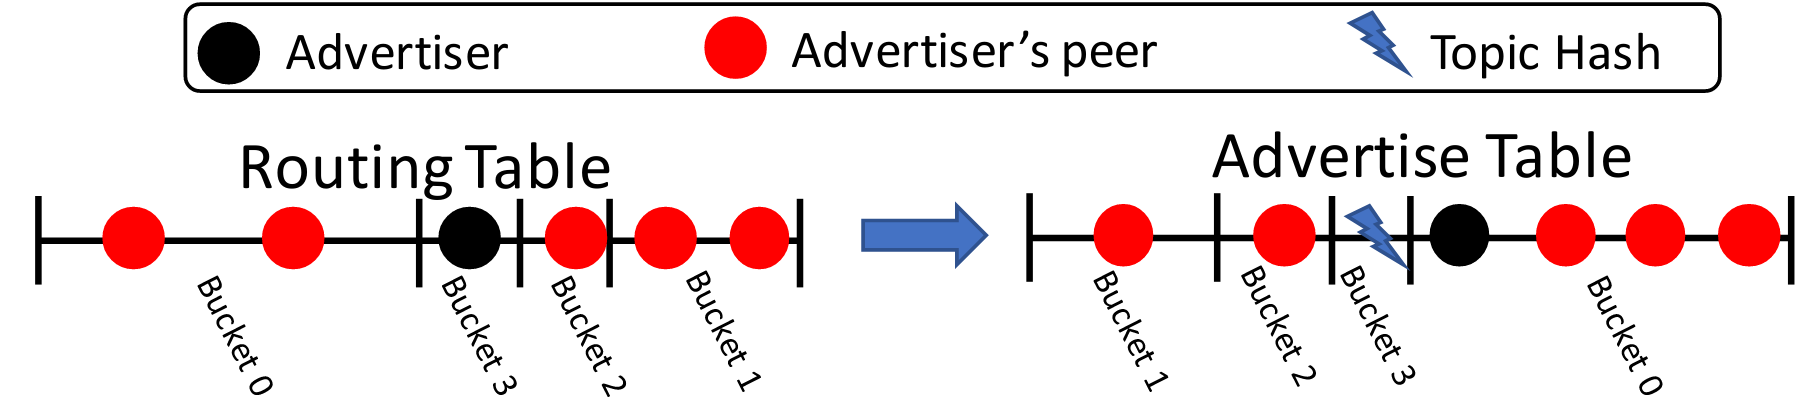
\includegraphics[width=0.45\textwidth]{img/tables}
    \vspace{-0.05in}
    \caption{Creation of an advertise table from a routing table.} %\mk{To be reworked and make it consistent with other figures. E.g., we shouldn't use a circle to represent the hash space. We can maybe also try to illustrate here the mechanism of placing a fixed amount of ads in each bucket.}}
    \label{fig:advertise_table}
    \vspace{-0.15in}
 \end{figure}

\para{Search Table}
The ad lookup process is supported by a \emph{search table}. 
Searchers maintain a separate table per topic they are currently looking for (\ie for each topic the client wants to start discovering nodes, a new \emph{search table} is created). 
Similar to the \emph{advertise table}, the \emph{search table} also stores k-buckets of registrar nodes by distance to the topic hash and buckets are initially filled from the local routing table organized by the distance from the topic hash.
\emph{Search table} buckets are also filled with new nodes discovered during the registration process.
%The \emph{k} factor of the search table should be relatively large to make the search efficient. 


\subsection{Distributing ads across registrars}\label{sec:registration_multi}
When an advertiser associates themselves with a topic, they start by creating a topic-specific \emph{advertise table} (as described above). 
Every peer present in the \emph{advertise table} is a potential registrar. 
The objective of the ad placement process is to continuously maintain $K_\textit{register}$ active (\ie unexpired) registrations in every bucket. 
Buckets located close to the topic hash cover less hash space than buckets located further away and, in turn, contain fewer potential registrars. 
Placing a fixed amount of ads per bucket, make registrars close to a topic hash more likely to receive registrations for that specific topic. 
Increasing $K_\textit{register}$, makes the advertiser easier to find at the cost of increased communication overhead. %More formally, the probability that a registrar has a topic-specific ad, based on the number of the nodes in a bucket $N_\textit{nodes}$, and the number of advertisers $N_\textit{advertisers}$ is given by:

%\begin{equation}
%   P_\textit{have ad} = 1-(1 - \frac{K_\textit{register}}{N_\textit{nodes}})^{N_\textit{advertisers}}
%\end{equation}
%\michal{TODO: Need to decide what to do with the equation above.}

For every bucket in the \emph{advertise table}, the advertiser selects
$K_{register}$ random peers and attempts to perform registration.
We describe details of the admission procedure in \Cref{sec:admission}. 
A successful registration places an ad on an advertiser for a fixed amount of time $a$.
If registration is unsuccessful (the selected registrar is down or refuses to store the ad), the advertiser selects another random peer from the same bucket and retries the registration process. 
The advertisers always maintain $K_\textit{register}$ attempts and/or
successful registrations per bucket unless there are less than $K_\textit{register}$ peers present in a specific bucket.
The advertiser repeats the process for every bucket in the \emph{advertise table}. 

The \emph{advertise table} is initialized with the peers already present in the routing table. It is thus possible that an advertiser will not know any nodes in buckets located close to the topic hash\footnote{This usually happens when the advertiser's ID is distant from the topic hash.}. 
To fill the empty buckets, the advertiser asks potential registrars to return $N$ closest peers to the topic hash they know of. 
The procedure is similar to the regular DHT \emph{FIND\_NODE} operation described in \Cref{sec:background}. 
The registrars respond with a list of peers regardless of the success of the registration operation. 
The advertiser uses the returned information to populate its \emph{advertise table}. 
As the advertiser progresses through the buckets, it queries potential registrars located closer to the topic hash and thus gets a more detailed view of this part of the network. 
Similar to the DHT routing, the registration procedure is guaranteed to find the closest node to the topic hash in the network within $O(log(N))$ number of steps. 

\subsection{Lookup operation}\label{sec:lookup}
To find ads, \sysname uses a process similar to the registration procedure. 
%The goal is to find $N_\textit{lookup}$ node advertised with a specific topic. 
%Each lookup requires a topic-specific \emph{search table} initially populated with nodes from the \emph{routing table}. 
Each lookup requires a topic-specific \emph{search table} described in \Cref{sec:struct}
The searcher progressively moves through buckets (starting from the furthest away), randomly chooses $K_\textit{lookup}$ registrars per bucket and sends them parallel lookup requests. 
Once received results from the first $K_\textit{lookup}$ selected registrars, other $K_\textit{lookup}$ registrars are selected from the following bucket with a smaller distance to the topic id.
The queried nodes are removed from the bucket.
Searchers stop the lookup procedure when they discover $N_\textit{lookup}$ peers. This is likely to happen far before reaching registrars located near the topic hash, especially for popular topics. As a result, \sysname avoids hot spots in the network and ensures fair load distribution. 
In case all buckets have been queried without finding enough nodes, the lookup process continues starting with the furthest distance bucket again. 
Once the lookup process is completed, the nodes are returned to the application.

Since the furthest buckets are also the largest (\ie it contains 50\% of all the honest registrars), an attacker placing malicious registrars in those buckets would require significant resources to eclipse the procedure. 
Searchers progressively moving towards smaller buckets near the topic hash guarantees successful discovery even for unpopular topics.
Each queried registrar responds with a list of $N_\textit{return}$ topic-specific advertisers the registrar knows of. 
If the total number of topic-specific registrations in the table is larger then
$N_\textit{return}$, the registrar should return a random subset.
While both $N_\textit{return}$ and $N_\textit{lookup}$ are protocol parameters,
the number of ads returned by a single registrar must be lower than the total
number of ads searchers are aiming to find $N_\textit{return} <
N_\textit{lookup}$. This is to diversify the sources of ads received by the searcher. \Ie, a single malicious registrar is not able to stop an honest searcher from contacting other nodes.
%\sergi{And is possible also a good idea to use a $N_\textit{lookup}$ parameter that forces that results from multiple buckets are used}
There is a trade-off between overhead and security when choosing $N_\textit{return}$ and $N_\textit{lookup}$. 
By requiring a large number of total ads to stop the search
($N_\textit{lookup}$) compared with the ads returned by the registrar
$N_\textit{return}$ a higher diversity of data sources is achieved at the cost of contacting a large number of registrars. On the other hand, similar values of both $N_\textit{lookup}$ and $N_\textit{return}$ reduce the overhead but increase the danger of a searcher receiving ads uniquely from malicious nodes. Finally, low values of $N_\textit{lookup}$ stop the search operation early, before reaching registrars close to the topic hash, contributing to a more equal load spread.
%However, for security reasons it is always recommendable to use $L_\textit{lookup}$, $N_\textit{return}$ and $N_\textit{lookup}$ parameters to ensure that at least 3 different registrars are queried from 2 different distance buckets.
%In the evaluation in \cref{sec:eval},  we set $L_\textit{lookup}=1$, $N_\textit{return}=10$ and $N_\textit{lookup}=30$, to be able to get results from 3 different registrars from 3 different buckets.
%\sr{Future work: investigate the impact of search parameters}

%\michal{For security, highlight that we want to mix results from different buckets and from different registrars - this is very important for security}
%\michal{Consider renaming search/advertise tables into search/registration caches}
%\michal{From Felix: 1) how exactly we choose the registrars to ask 2) filling the search table as you go 3) how many queries per node, how do you combine the results 4) when do you stop}
%\ramin{In practice, is $N_\textit{lookup}$ a parameter that can be controlled? It sounds like something application-specific, e.g. for some applications, it might be enough for a searcher to just find one node to be able to use the application as intended. Search for 10 and choose one randomly from them?}
%\michal{That's a good point. Not sure if we should allow the application to control both $N_\textit{lookup}$ and $N_\textit{return}$. Or maybe fix a ration between both and automatically set $N_\textit{return}$ once $N_\textit{lookup}$ is chosen by the application.}
%\sergi{I think $N_\textit{return}$ should not be configurable since it is limited by the maximum number of nodes returned in a message which i think is 16.  I think $N_\textit{lookup}$ can be configurable, but never smaller than a value multiple of $N_\textit{return}$}



\section{Registration Protocol}\label{sec:registration}
In this section, we describe a registration procedure followed by an advertiser to place an ad on a specific registrar. 
\subsection{Data Structures}
\para{Advertisement}
When advertisers send a registration request, they send an \emph{advertisement} (\emph{ad} in short). The ad contains the IP address of the advertiser, the ID of the advertiser, the topic the ad is for and additional information needed to later contact the advertiser (\eg an application-specific port number). In the remaining part of the paper, we omit the additional information for brevity. 

\para{Topic Table}
Registrars store received ads locally in a data structure called a \emph{topic table}. Each ad stored in the topic table has an associated expiry time, after which the ad is automatically removed. Once an ad is added to the table, the expiry time is set to a fixed value $a$. The topic table acts as a \emph{first in, first out} queue for ads. The total size of the topic table is limited by $C_\textit{topic\_table}$. \sysname does not impose topic/IP/ID-specific limits on the content of the \emph{topic table}. 
A single advertiser may place at most one ad for a specific topic in the topic
table (registration requests for ads already in the table are ignored).
However, an advertiser may attempt to place ads for multiple topics at the same registrar.

\para{Ticket}
Tickets are immutable objects issued by registrars to advertisers when receiving a registration request. Each ticket contains:
\begin{itemize}
    \item Ad - repeated registration request (as described above). 
    \item Initial timestamp - the local time at the registrar when the ad was received for the first time, $t_\textit{init}$
    \item Waiting time - the waiting time calculated by the advertiser for the ad, $t_\textit{waiting}$. We describe the details on waiting time calculation in \Cref{sec:waitingTime}. 
\end{itemize}
The tickets are digitally signed by the issuing advertiser. 

\subsubsection{Registration Procedure}
An advertiser willing to register an ad at a registrar starts by sending an
initial request uniquely containing its \emph{advertisement}. Based on the
content of the topic table and the registration, the registrar calculates an
ad-specific waiting time. The advertiser then issues a ticket including the
calculated waiting time and the time of receiving the initial request and sends it back to the advertiser.

The advertiser waits for the indicated time and attempts to register again. The consecutive registration request must include the last ticket issued by the registrar. Tickets can be used uniquely during a registration window:
% I dont think this equation is correct, surely not two $t_{init}$'s.
\begin{equation}\label{eq:registration_window}
    t_\textit{window} = [t_\textit{init} + t_\textit{waiting}, t_\textit{init} + t_\textit{waiting} + t_\textit{init} + \delta t_\textit{window}]
\end{equation}
All the registration requests outside the registration window are ignored by the advertiser. The registrar calculates the registration windows based on the content of the ticket. $\delta t_\textit{window}$ should be chosen to accommodate for the maximum delay between the advertiser and the registrar. 

The advertiser calculates a new waiting time, based on the current content of
the topic table, every time it receives a registration request (with or without
ticket). The waiting time in the ticket is used only to calculate the
registration windows and prevent advertisers from trying to register
continuously. The ticket also allows the calculation of an accumulated waiting time:
\begin{equation}
    t_\textit{cumulative} = \textit{now} - t_\textit{init}
\end{equation}
An ad is admitted iff the accumulated waiting time is equal or larger than the calculated waiting time $t_\textit{cumulative} \ge t_\textit{waiting}$\footnote{Note that a registration request without a ticket may be admitted directly if $t_\textit{waiting}=0$.}. For registration requests without a ticket $t_\textit{cumulative} = 0$. An advertiser that misses its registration window (as specified by the most recent ticket), loses all its cumulative waiting time and must attempt to re-register without a ticket (\Cref{fig:ticket_validity}). Once an ad is admitted, the registrar confirms the registration to the advertiser.

If the cumulative time is not sufficient, $t_\textit{accumulated} < t_\textit{waiting}$, the registrar issues a new ticket and the advertiser repeats the whole procedure. With consecutive registration attempts, advertisers increase their cumulative waiting time $t_\textit{cumulative}$ and eventually will be admitted. 



\begin{figure}
    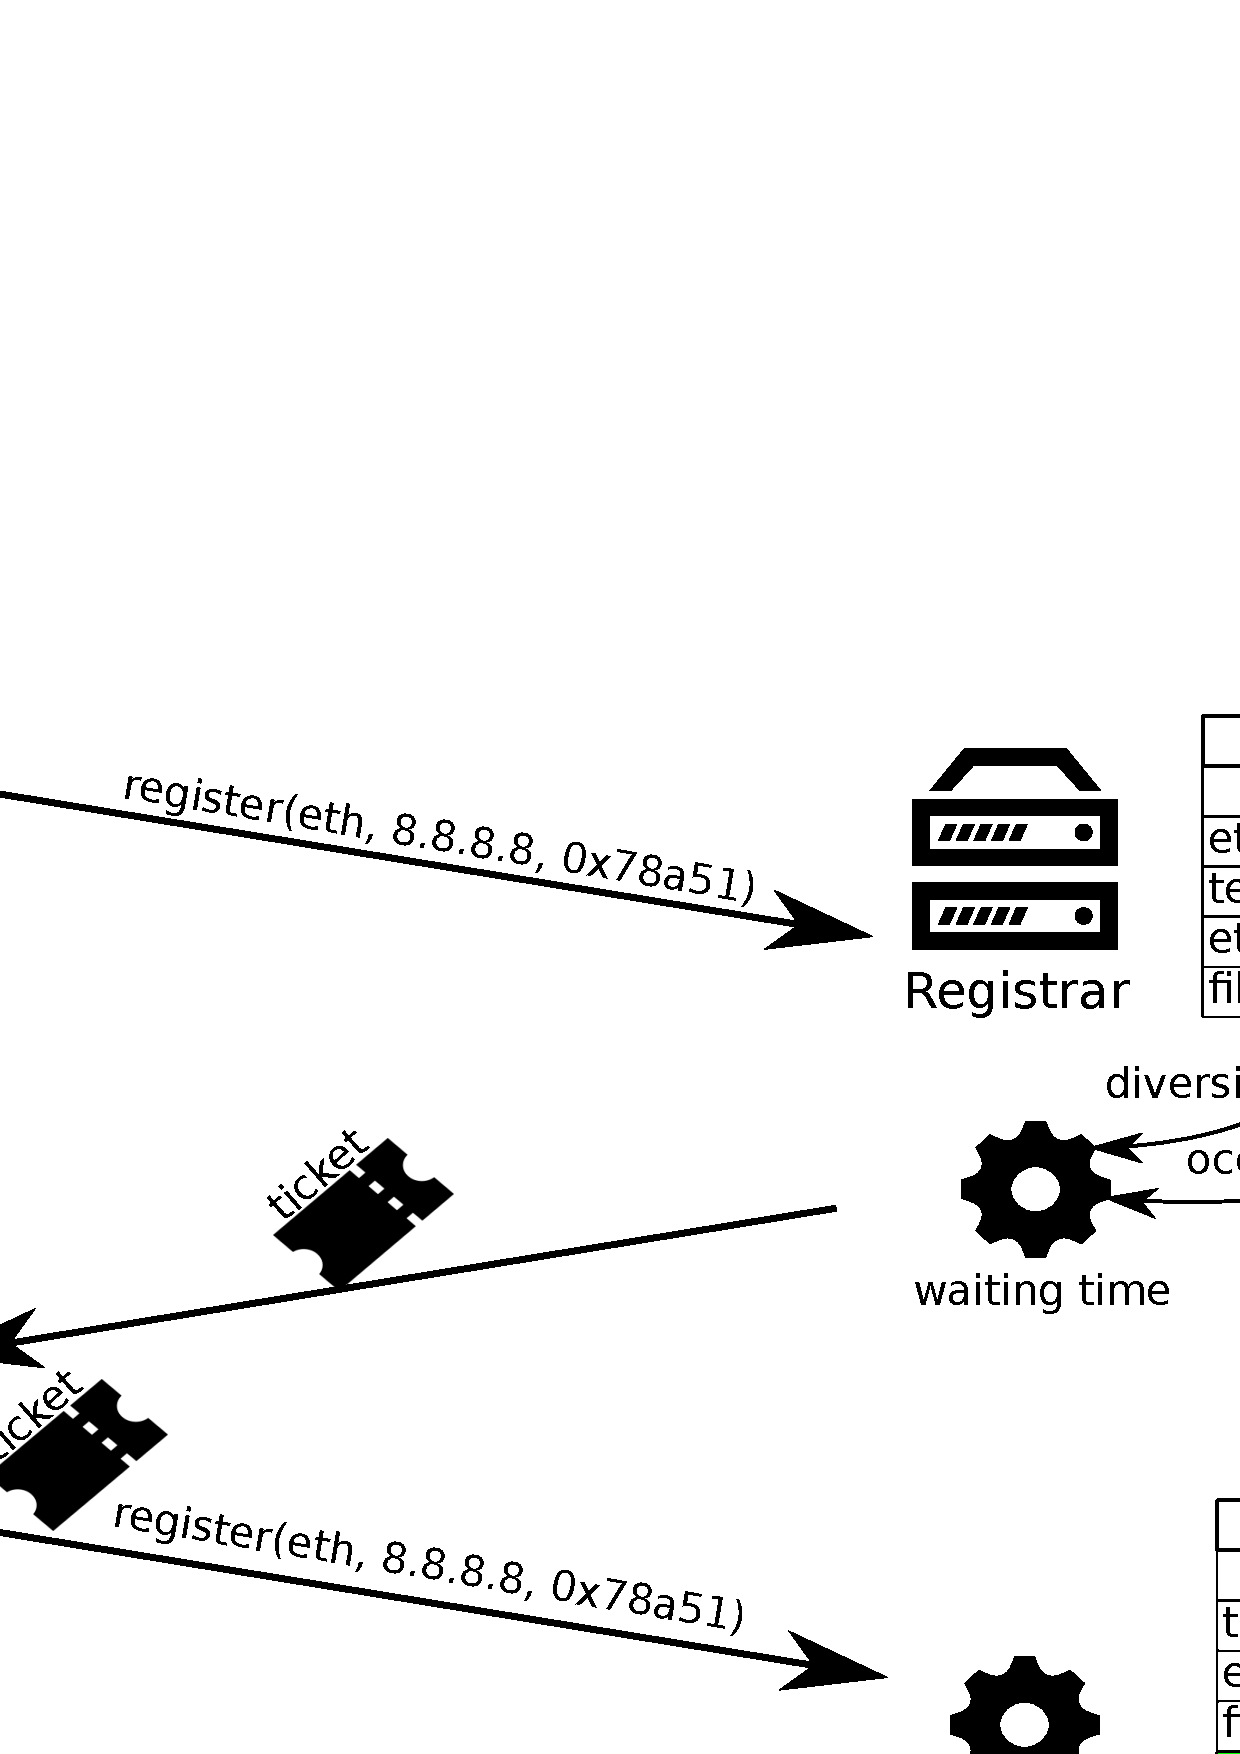
\includegraphics[width=0.5\textwidth]{img/registration}
    \caption{Registration operation.}
    \label{fig:registration}
\end{figure}

The inclusion of issue-time allows the registrars to prioritise advertisers
that have been waiting the longest, as we explain later. Because the tickets
are immutable (i.e., tampering with the ticket is detectable by the registrars
that originally issued the ticket), when a registrar issues a new ticket (in
case a registration is not immediately successful) to an advertiser, the
registrar simply copies the issue-time from the last issued ticket and uses that as the issue-time of the new ticket. This means that the registrars are not required to maintain any state for each on-going ticket request given that they can simply verify the authenticity of the ticket in the incoming registration requests.


    
\begin{figure}
    \includegraphics[width=0.5\textwidth]{img/ticket-validity}
    \caption{Ticket validity period.}
    \label{fig:ticket_validity}
\end{figure}

An advertiser gives up and stops the registration process with a registrar when
it receives $r$ unsuccessful registration attempts (i.e., after being issued $r$
tickets without being admitted). In this case, the advertiser removes the registrar from its registration table and selects a new node located in the same bucket and attempts a new registration procedure.
%\michal{Is the below true? Shouldn't we try to register at the same node?}
%\sergi{We dont use the same, we pick another randomly. we could use the same but i think for diversity could be better  this way}
Similarly,  after the expiration of a previously placed ad the node is removed from the ticket table and the process is restarted with a new node picked from the local table.
\ramin{Confirmation message contains expiration time?}
\michal{Good point. We assumed a common expiration time so didn't include it in the response. But it might be good to either clarify that or include the expiration time in the response.}

%\michal{We're mixing here single-registrar registration process. It should be covered in the first section.}
%In our approach,  advertisers start a limited number of parallel registrations in each ticket table bucket distance.
% More specifically, an advertiser follows the below steps to distribute its ads for a specific topic:
%\begin{enumerate}
     %\item The advertiser (\hl{randomly?}) selects a set of K registrar nodes from each bucket distance of the ticket table structure, where the number of bucket distances (B) is a configurable parameter of the ticket table.
%    \item The advertiser selects a K random of node.,  by querying the local Ethereum routing table,  for each bucket distance.
    %\item A TICKETREQUEST message is initially sent to each of the selected registrar nodes in the previous step.
%    \item Registrar node replies with a TICKETRESPONSE.  This message includes the TICKET which contains a waiting time and a ticket issue time.  The TICKET is stored in the table.
    %\item The advertiser replies after the waiting time expires with a REGTOPIC request containing the previously received TICKET attached to it.
    %\item After the TICKET reception the waiting time is calculated again at the registrar.  A registration is successful when the waiting time calculated at the registrar is smaller than the cumulative waiting time,  which means that the advertiser has waited long enough.
    %\item The registrar sends a REGCONFIRMATION response to the advertiser of the successful registration. In general, the topic table occupancy is guaranteed to always remain below the topic table capacity by the waiting time calculated: the waiting time function returns increasingly large values as the topic table space runs out; the waiting time becomes infinite in case there is no space.
    %\item In case the new calculated waiting time is not smaller than the cumulative waiting time, the registration is not successful and the registrar replies with a REGRESPONSE message containing a new TICKET (containing a new waiting time).
    %\item 
%\end{enumerate}



%Reasonable \texttt{topic table capacity} is 50,000 ads. 
%Since ENRs are at most 300 bytes in size, these limits ensure that a full topic table consumes approximately 15MB of memory.
%The topic table is shared across multiple advertisers and stores topics with varying popularity (which is determined by how many nodes register the topic) among the participants of \sysname. 
%It is important that the high popularity of a particular topic should not prevent peers from registering less popular topics. 
%This is achieved using the waiting time function that will determine the time an advertiser will have to wait to place an ad after a ticket request,  and is detailed in Section~\ref{sec:waitingTime}.



%storing arbitrary information determined by the issuing registrar node.  While details of encoding and ticket validation are up to the implementation, tickets must contain enough information to verify that:
%\begin{itemize}
%    \item The advertiser attempting to use the ticket is the one which originally requested it.
%    \item A ticket is valid for a single topic only.
%    \item A ticket can only be used within the 'registration window' (explained below).
%    \item A ticket can not be used more than once.
%\end{itemize}

%In addition to the waiting time,  the sequence of tickets issued by a registrar for a specific advertiser also records the original issue-time of the first ticket which can be used to compute the cumulative waiting time so far; that is, the time elapsed since the advertiser requested its first ticket to place its ad. 



%\michal{Change the markdown notation of variables (CAPACITY) to scientific (n)}
%Any REGTOPIC messages that are not sent during the registration window determined by the waiting time (indicated in the ticket),   (as seen in Figure \ref{fig:ticket_validity}) are ignored by the registrars.  
%If the advertiser comes back during the established registration window,  the advertiser can either place the ad (and notify the advertiser of a successful registration) or issue another ticket with a new waiting time in another ticket response message. 
%An advertiser may be given one or more tickets in a sequence before a successful registration,  and this means that overall the advertiser waits for a 'cumulative waiting time' period that is the sum of multiple waiting times issued in each ticket in the sequence before finally registering an ad. 
%Assignment of 'waiting times' is the only way the registrars can control the registrations in order to both:

%\begin{itemize}
%    \item Throttle ad placement rate to prevent overflowing of topic table: when the topic table is full, the advertisers must wait for already placed ads to expire first before they are allowed to register new ads.
%    \item Prioritise registrations to achieve a diverse set of ads in the topic table. For example, registrations for less popular topics or registrations from advertisers that increase IP diversity (in the set of advertiser IP addresses that currently have an ad in the table) can be prioritised over others. This is useful to reduce the impact of Sybil attacks on the service discovery system.
%\end{itemize}

%Waiting times will be calculated according to a 'Waiting time function' detailed in Section~\ref{sec:waitingTime}.  Enforcing this time limit prevents misuse of the topic table because any topic must be important enough to outweigh the cost of waiting for ad placement. Imagine a group phone call: announcing the participants of the call using topic advertisement isn't a good use of the system because the topic exists only for a short time and will have very few participants. The waiting time prevents using the topic table for this purpose because the call might already be over before everyone could get registered. Also, it prevents attackers from overflowing topic table by regulating registrations in case of spamming attacks.



%The registrars ensure the authenticity of the tickets they issue to the advertisers through symmetric encryption we explain below.


%\input{sections/recap}
\section{Waiting Time}
\label{sec:waitingTime}

\mk{To consider - also add a challenge subsection here?}

The waiting time function is used to calculate the total time advertisers have to wait before being admitted to the ad cache. 
The function directly shapes the structure of the ad cache,  determines its diversity and performs flow control. 
It also protects against attacks, where a malicious actor tries to dominate the ad cache and exhaust resources of the registrar. 

Each request is given a waiting time based on the IP address of the registrar, the topic of the request and the current state of the ad cache. 
The waiting time function is divided into three parts: \emph{const} (constant
for all the requests), \emph{occupancy score} (ranging from $0$ to $\infty$)
and  \emph{similarity score} (ranging from $0$ to $2$). The final result is a
product of all three:
\begin{equation}
\label{eq:global}
w = \emph{const} \times \textit{occupancy score} \times \textit{similarity score}. 
\end{equation}

The \emph{const} part determines the absolute values of the returned waiting time and is given by:
\begin{equation}
\label{eq:const}
    \textit{const} = ba
\end{equation}
where $a$ is the \emph{ad lifetime} (the amount of time each ad spends in the
ad cache), and $b$ is a system parameter. Higher values of $b$ result in
higher returned waiting times and lower average occupancy of the ad cache.\mk{TODO:refer to the analysis when it's done}
Furthermore, a good value of $b$ allows protection against admitting similar advertisements when the \emph{similarity score} is low (\ie when the cache is almost empty).\mk{Maybe we should signal we do determine "the good value" later on?}

The \emph{occupancy score} is based uniquely on the number of the ads already in the cache.
Its role is to progressively increase the waiting time as the ad cache fills up and to limit the memory used by a registrar.
The \emph{occupancy score} is defined by equation~\ref{eq:occupancy}:

\begin{equation}
\label{eq:occupancy}
    \textit{occupancy score} = \frac{1}{(1-\frac{d}{n})^{P_{occupancy}}}
\end{equation}
where $d$ is the number of ads in the cache, $n$ is the capacity of the cache. $b$ and $P_{occupacy}$ are protocol configurable parameters. 
When the number of ads in the cache is low ($d \ll n$ ), the \emph{occupancy score} goes to $1$. 
As the ad cache fills up, the score will be amplified by the divisor of the equation. 
The higher values of $P_{occupancy}$, the faster the increase. 
With the current occupancy $d$ close to the capacity of the cache $n$, the \emph{occupancy score} goes to infinity thus limiting the number of admitted requests.\mk{the above might go to the analysis}

The role of the \emph{similarity score} is to determine how similar is the incoming request to the ads already in the ad cache in terms of the IP address and the topic. 
Requests significantly different from the current content of the cache receive lower similarity score resulting in lower overall waiting time. 
Such an approach promotes fairness across topics (it is easier for less popular topics to get into the cache) and protects against attempts to fill the ad cache by a small number of advertisers (as identified by their IP addresses). The similarity score is defined as a sum of similarity score for IP and the topic of the request: $\textit{similarity} = \textit{similarity(IP)} + \textit{similarity(topic)}$. 

The similarity score for topics is given by equation~\ref{eq:similarity}:
\begin{equation}
\label{eq:similarity}
    \textit{similarity(topic)}= \frac{d(topic)}{d}
\end{equation}
where $d(topic)$ is the number of ads for the specified topic already in the cache and $d$ is the total number of ads in the cache. 
The score goes to $1$ as the specified topic dominates the cache $d(topic)  \approx  d$. 

%For calculating the IP address diversity \sysname uses a different similarity score. 
A simple similarity score used for topics cannot be securely applied for IP addresses. 
An attacker may be able to generate a large number of different addresses sharing the same prefix (\eg using a single /24 IPv4 network) that, while similar, would receive low \emph{similarity scores}. 
The Go Ethereum client~\footnote{https://github.com/ethereum/go-ethereum} limits the number of IP addresses coming from the same (\eg /24 IPv4 address) network.
However, it is impossible to reliably set those limits without knowledge about the network size or NAT configuration of honest nodes. 
Instead, we propose an approach that directly captures the similarity level across different IPs and translates it into a numerical score. 

We introduce a binary \emph{tree}, as shown on \Cref{fig:ip_tree}, that stores IP addresses used in the existing registrations in the ad cache.
Each node stores a counter, while the edges represent consecutive $0$s or $1$s in a binary representation of IP addresses.
For simplicity,  we present the \emph{tree} for IPv4 addresses but its adaptation for IPv6 is straightforward.

\begin{figure}
    \includegraphics[width=0.45\textwidth]{img/ip_tree}
    \caption{Inserting an IP address into the IP \emph{tree} structure. \mk{TODO:make it up to date, smaller and consistent with other figures.}}
    \label{fig:ip_tree}
\end{figure}

Apart from its root,  the \emph{tree} consists of 32 levels (33 levels in total) representing bits in the binary representation of IPv4 IP addresses. 
The root level is depicted as level $0$, the level of its successor as level $1$ and so on. 
The counter of every \emph{tree} node is initially set to $0$. When adding an IP to the \emph{tree},  the address is first converted to its binary representation and follows a path in the \emph{tree} corresponding to consecutive bits. 
Counters of all the visited nodes are increased by $1$. 
As a result, the root counter stores the number of all the IP addresses in the ad cache, its $0$ successor stores the number of the IP addresses starting with $0$, its $1$ successor stores the number of the IP addresses starting with $1$ and so on. 
Removing an IP from the \emph{tree} follows the analogical procedure but decreases all the counters on the path. 

\mk{The following is out of date - need to describe the current approach}
After each addition of an address to the \emph{tree} a score is generated.
The score is a sum of \emph{penalty points} of obtained on visited nodes. 
$$score(IP)=\sum_{i=1}^{32} \textit{penalty}(p_{\geq i}) $$
where $p_{\geq i}$ is the number of IP addresses in the cache sharing a prefix with $IP$ with a length of at least $i$. A penalty point is given at $p_{\geq i}$ if the IP address to be added makes the tree more unbalanced than the tree currently is:

\begin{equation}
    \textit{penalty}(p_{\geq i})=
    \begin{cases}
      0, & \text{if}\ p_{\geq i} \leq \frac{p_0}{2^i} \\
      1, & \text{otherwise}
    \end{cases}
  \end{equation}

The counter values are taken \emph{before} the increment caused by adding the address\footnote{The first added address will thus always have a score of $0$}. 
Finally, the similarity score for an IP is normalized by the length of the IP address (and thus the maximum possible number of the penalty points):
\begin{equation}
    \textit{similarity(IP}) = \frac{\textit{score(IP)}}{32}
\end{equation}

Similarly to the topic score, the IP similarity score ranges from $0$ to $1$ and returns values closer to 1 for different addresses sharing the same prefix (the longer the shared prefix, the higher the score).

The final formula for the waiting time function can be represented with  the following formula,  adding all \emph{similarity scores} and multiplying by the \emph{occupancy score}:

\begin{equation}
\begin{split}
    \textit{w(IP, topic)} = 
    ba(\frac{\textit{score(IP)}}{32} +
    \frac{d(topic)}{d})
    \frac{1}{(1-\frac{d}{n})^{P_{occupancy}}}
\end{split}
\end{equation}

The formula can be simplified like in equation~\ref{eq:simp}, where ss determines the the \emph{similarity score} and os the \emph{occupancy score}.

\begin{equation}
\label{eq:simp}
    \textit{w(IP, topic)} = 
    (\textit{ss(IP)} + 
    \textit{ss(topic)})
    \textit{os()}
\end{equation}

\subsection{Lower Bound}
With the waiting time formula, every change in the registrations stored in  the ad cache may increase or decrease waiting times of other requests. 
Therefore,  an advertiser receiving waiting time $w(t_1)$ at time $t_1$, may get a smaller waiting time $w(t_2)$ at time $t_2$ ($t_1 < t_2$) in case the situation of the ad cache is very different (\eg when an ad for the same topic expires between $t_1$ and $t_2$). 
As a result,  advertisers willing to minimize their waiting time can be incentivized to keep checking the waiting time as frequently as possible hoping for a better one.
However, this can be a problem. 
Registration ticket requests should be kept to the minimum and an incentive for constantly spamming ticket requests to get a better waiting time can overload a network and can lead to some nodes getting better performance than the rest.
Thus, we have designed a mechanism to avoid the case that any node who is already in possession of a ticket with a determined waiting time, can get a better waiting time (including the new waiting time and the time passed between the first ticket request and the subsequent) by issuing new ticket requests.
One solution to this problem is to take into account all the expiration times when calculating the waiting time. 
However, such a solution is computationally expensive (\eg $O(n)$) and unfeasible in practice.

\begin{figure}
    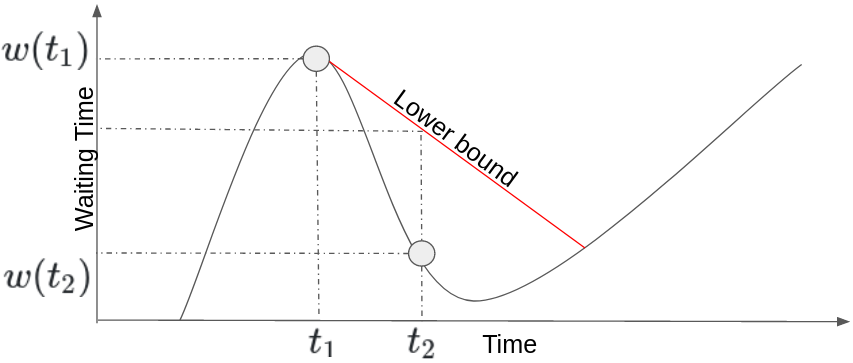
\includegraphics[width=0.45\textwidth]{img/lower_bound.png}
    \caption{Waiting time lower bound.}
    \label{fig:lower_bound}
\end{figure}

When asking for a new waiting time before the previously obtained one elapses,
an advertiser loses its already accumulated waiting time. This means that
asking for a new waiting at time $t_2$ can lower the overall waiting only if
the new waiting time $w(t_2)$ is smaller than $w(t_1)$ by more than $t_2 - t_1$: $w(t_1) - w(t_2) < t_2 - t_1$.
To make sure this is not the case, our protocol enforces a lower bound on the
waiting time. \Ie we make sure that an advertiser's waiting time received at
$t_2$ is not smaller than the waiting time at $t_1$ ($t_1 < t_2$) by more than
$t_2 - t_1$ (\Cref{fig:lower_bound}).
However, holding such a bound for every request (\ie every combination of IP/topic) would cause significant memory overhead ($O(|IPs|\times|topics|)  \gg O(d)$) and would present an easy way for an attacker to create state at the registrar. 

To store the lower bound in a more efficient way, we rewrite the waiting formula as a sum of topic/IP distinctive parts:

\begin{equation}
    \textit{w(IP, topic)} = 
    \textit{ss(IP)}\textit{os()} + 
    \textit{ss(topic)}\textit{os()}
\end{equation}
Ensuring that the lower bound is enforced for each of the three components
makes sure that the total waiting will respect the lower bound as well. At the
same time, it only requires storing the lower bound for every IP/topic and not all their combinations. This approach reduces the memory overhead to $O(|IPs|+|topics|) = O(d)$.

For each of the components above IP, and topic present in the cache, we
keep a bound. When a specific IP enters the cache for the first time, bound(IP)
is set to 0 and a timestamp(IP) is set to the current time. When a ticket
request arrives from the same IP, we calculate the IP waiting time $w_{IP}$ and
return the value, $w_{IP} = max(w_{IP}, bound(IP) - timestamp(IP))$. It makes sure that advertisers never receive a better time by frequently requesting new tickets. The bound and the timestamp are updated when a new ticket is issued and $w_{IP} > (bound(IP) - timestamp(IP))$. The same holds for topics.
\mk{TODO: @Onur we need to introduce the waiting time in the tree I believe}




%!TEX root = ../main.tex
%=========================================================

\section{Performance Evaluation}
\label{sec:eval}

We evaluate the \sysname prototype and answer the following research questions:
\begin{enumerate}
    \item What is the overhead introduced by \sysname's register and lookup operations? How does it compare to the current Discv4 system and vanilla DHT-based solutions?
    \item Does \sysname provide high performance for all the topics regardless of their popularity? What is the load distribution across network participants?
    \item How do malicious nodes impact \sysname’s performance? How difficult is it to launch eclipse and DoS attacks against the system?
\end{enumerate}

\para{Setup} We implemented \sysname in PeerSim~\cite{p2p09-peersim}, a large-scale peer-to-peer network simulator. 
We used an existing vanilla Kademlia implementation~\cite{peersim_kademlia} as a starting point, extend it to make it equivalent to the existing Ethereum DHT (as described in \Cref{sec:background}) and build \sysname on top of it. 
Firstly,  we compare our system against the current Ethereum \discv discovery service\footnote{https://github.com/ethereum/devp2p/blob/master/discv4.md}.
In \discv, the DHT is not used as a key/value store but just a way to discover other nodes in the P2P network. 
\discv issues 3 lookups to random destinations using a simple Kademlia lookup,  and it stores all found nodes during the  \emph{random walk} in a buffer. 
Nodes are consumed from the buffer by upper-layers of the Ethereum protocol (RLPx~\footnote{https://github.com/ethereum/devp2p/blob/master/rlpx.md})
when trying connections to new nodes, and when the buffer is empty new lookups are started to other 3 random nodes.
We also compared \sysname against  a traditional key/value store implemented on top of the DHT (similar to the content routing system that IPFS is currently using by default~\cite{libp2p_kaddht} to find providers for a specific content),  where advertisements are stored on the N nodes with identifiers with a smallest distance  to the topic hash.  
We evaluated the traditional key/value store implementation, using our admission protocol (\Cref{sec:waitingTime}) to accept incoming registrations,  naming it \altnameticket, and also without any admission protocol were registrations are replaced using  Last Recently Used policy, named \altname.
When using \altname and \altnameticket, there is no \emph{registration table} that keeps track of ongoing registrations and new registrations are periodically issued by nodes every advertisement period.
The topic lookup for \altname and \altnameticket is similar to the \discv lookup.  When a node performs a lookup selects the 16 closest nodes to the topic hash from the local routing table and it sends topic query messages to the first  $\alpha=3$.
In the reply, queried nodes attack the known nodes for the specific topic but also known nodes to the same distance of the topic hash. 
The known nodes for the specific topic are stored in the lookup buffer. 
The known nodes with the same distance to the topic id are added to the list of 16 closest nodes,  which is reordered and keeps only the 16 closest.
The lookup process is ended when all 16 closest nodes are queried or when enough nodes are discovered for the queried topic, which is defined by the system parameter $N_\textit{lookup}$ 


 The simulator reports the following performance metrics. 
 \begin{itemize}
     \item \textbf{Message Overhead} - the number of messages received by each node. We calculate separate values for both lookup and registration operations. Higher values mean larger strain put on each nodes and increased time to complete each operation. 
     \item \textbf{Discovered Peers} - the number of application-specific peers discovered by searchers during lookup operations. Each operation is finished after discovering 30 nodes. The metric allows to verify whether each searcher can discover its peers.
     \item \textbf{Discovered By} - the number of searchers each advertiser was discovered by. This metric allows us to verify whether each peer is being discovered and how the number of discoveries differs across peers.
%     \item \textbf{Placed Registrations} - the number of registration placed by each advertiser. 
%     \item \textbf{Accepted Registrations} - the number of registrations each  registrar accepted. It allows to verify the load on each registrar and analyse the their load distribution.
 \end{itemize}
 %We calculate per-node average for the metrics above and report their standard deviation.  Note that \emph{Discovered Peers} and \emph{Discovered By} metric will have the same average vales, but will vary in standard deviation. The same applies to \emph{Placed Registrations} and \emph{Accepted Registrations}. 
 
In the simulations, we verify the impact of the following parameters:
 \begin{itemize}
     \item \textbf{Network Size} - the number of all the nodes being part of the application-agnostic Ethereum DHT. We set the default value to 25000, as reported by the official Ethereum crawler~\cite{discv4-dns-lists}. Each nodes receives an IP address and ID as reported in the crawled ENS records. We calculate an average network churn between daily crawls equal to 3\% with the same increase to accommodate for nodes going off and back online between the scans. 
     \item \textbf{Topic Number} - the number of distinct applications using the Ethereum DHT evaluated are between 50 and 600. We set its default value to 300, similarly to the data collected from the Ethereum DHT and shown in Figure~\ref{fig:ecosystem}, using a Zipf distribution with an exponent 1.0.  Each node only participates in a single topic.
     \item \textbf{Malicious nodes} - the number of malicious participants of the Ethereum DHT to evaluate the resistance against sybil attacks are between 250 and 2500 nodes,  using 1000 for the default value.  Each malicious node receives a distinct identifier, that can be generated following either a random uniform distribution,  or generated to obtain identifiers with the minimum distance to the topic hash that is targeted in the attack.
     \item \textbf{Malicious IPs} - the number of IP addresses available to the attacker to be shared between the malicious nodes. We set its value between 10 and 1000,  using 100 for the default value.  Meaning that every 25 malicious nodes will share a single, random IPv4 address in the best case or every malicious node will use a different IP address in the worst case.  
In the simulations we use only IPv4 addresses since, at the moment of writing this paper,  we analysed  Ethereum DHT and we found out 99\% of the nodes use IPv4.
 \end{itemize}
\sr{To add $N_\textit{lookup}$  and $N_\textit{returned}$ used}
 
Each simulation takes 1h of simulated time during which each advertiser tries to constantly maintains its registration and performs a single lookup operation uniformly spread across the simulation time.  For \sysname and DHT-based solution, we set the \emph{registration table} capacity to 500  to align with the memory requirements from the official Ethereum DHT implementation, and the advertisement period is set to 15 min, \ie every 15 min registration expires in the registrars. 
We set all the DHT-related parameters to the default values from the current Ethereum DHT: 17 buckets and 16 node in each bucket.
 \sysname parameters have the following values: number of registrations placed per bucket $K_{register}= 3$, $P_{IP} = $, , $P_{ID} = $, $P_{topic} = $, $P_{occupancy} = $,  $L_\textit{lookup}=1$, $N_\textit{return}=10$ and $N_\textit{lookup}=30$. 
They were selected based on extensive simulations that we skip due to the space limitation but included in our Github repository~\cite{our_repo}. 

%%%%%%%%%%%%%%%%%%%%%%%%%%%%%%%%%%%%%%%%%%%%%%%%%%%%%%%%%%%
\subsection{Message Overhead}

\sr{TODO: detail what violin plot represents exactly}

In~\Cref{fig:regMsgsPerTopic}~and~\Cref{fig:regMsgsPerSize},  we can observe the distribution of the total number of messages received per node related to the registration process, \ie registrations requests and replies during simulation time,  for different network sizes and different number of topics in the network.
Both figures show no values for \discv protocol,  since  \discv nodes do not receive any registration message because they do not participate to any topic-based registration process.   \discv can only find nodes doing  \emph{random crawls} in the DHT  without being able to do topic specific queries. 

\begin{figure}
\centering
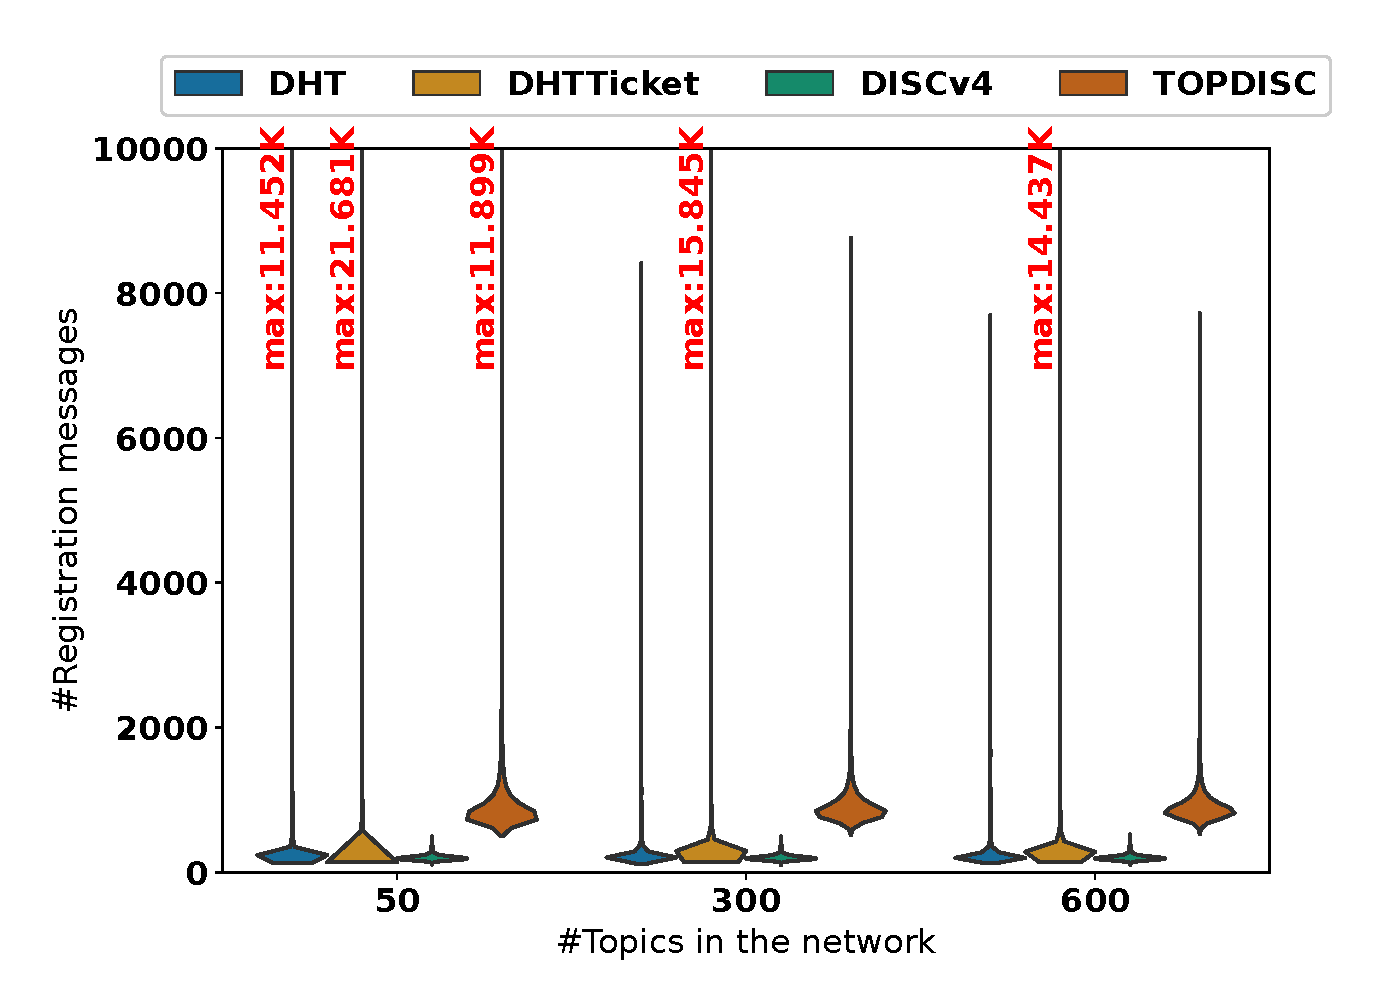
\includegraphics[width=\linewidth]{results/efficiency/violin_topic_registrationMsgs.eps}
\caption{Y-axis: Distribution of registration related messages received by peers for varying number of topics for the simulation time.}
\label{fig:regMsgsPerTopic}
\end{figure}

In~\Cref{fig:regMsgsPerTopic}~and~\Cref{fig:regMsgsPerSize},  we can observe while most of \sysname nodes receive around 500 registration messages,  with just a few receiving up to 5k messages in the worst case,  \altname solutions are more spread between 0 and 1000 received messages, but with some peaks up to 43k messages,  an order of magnitude higher than \sysname.
This is caused by the fact that all nodes in \altname solutions try to put registrations starting by the closest nodes to the topic hash,  creating an uneven distribution  towards these nodes. 
In \sysname, the use of \emph{registration table} for advertisement placement provides a similar effect. 
However this effect is diminished by the use of waiting times to regulate advertisement placement.  The increase of waiting time in the more congested nodes, causes that nodes starts more registrations in less congested nodes limiting the number of registrations placed on nodes close to topic hash.
This effect is not seen when using \altname combined with tickets. 
This is due to the fact that \altname is not using a \emph{registration table} to keep track of ongoing registrations.  Because of this,  advertisers start new registrations towards the topic hash every advertisement period, even if they did not succeed in the previous attempts due to high waiting times.
Therefore using tickets in the \altnameticket, maybe useful to increase the diversity in the \emph{registration tables} but not for load balancing between nodes.

When increasing the number of topics in the network (\Cref{fig:regMsgsPerTopic}), it is not observed an increase of registration messages for any of the different protocols. 
However,  when increasing the number of nodes participating in the network (\Cref{fig:regMsgsPerSize}),  also registrations messages received per nodes are increased, as expected.
But this increase is very different between \sysname and \altname protocols.
\sr{tbc with specific values}

\begin{figure}[!h]
\centering
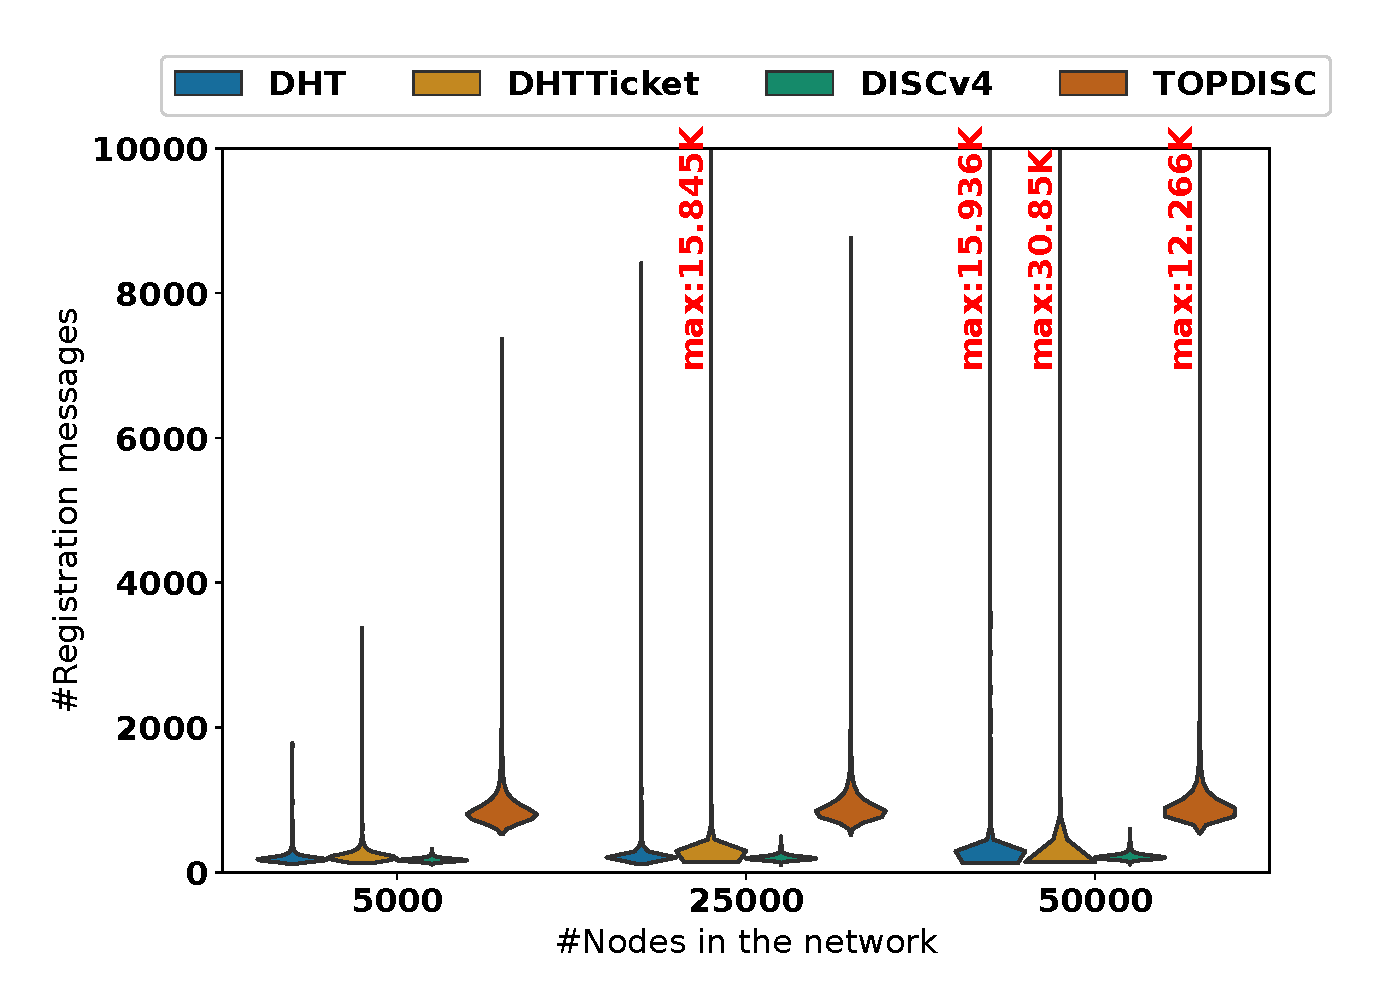
\includegraphics[width=\linewidth]{results/efficiency/violin_size_registrationMsgs.eps}
\caption{Y-axis: Distribution of registration related messages received by peers for different network size for the simulation time.}
\label{fig:regMsgsPerSize}
\end{figure}

\begin{figure}
\centering
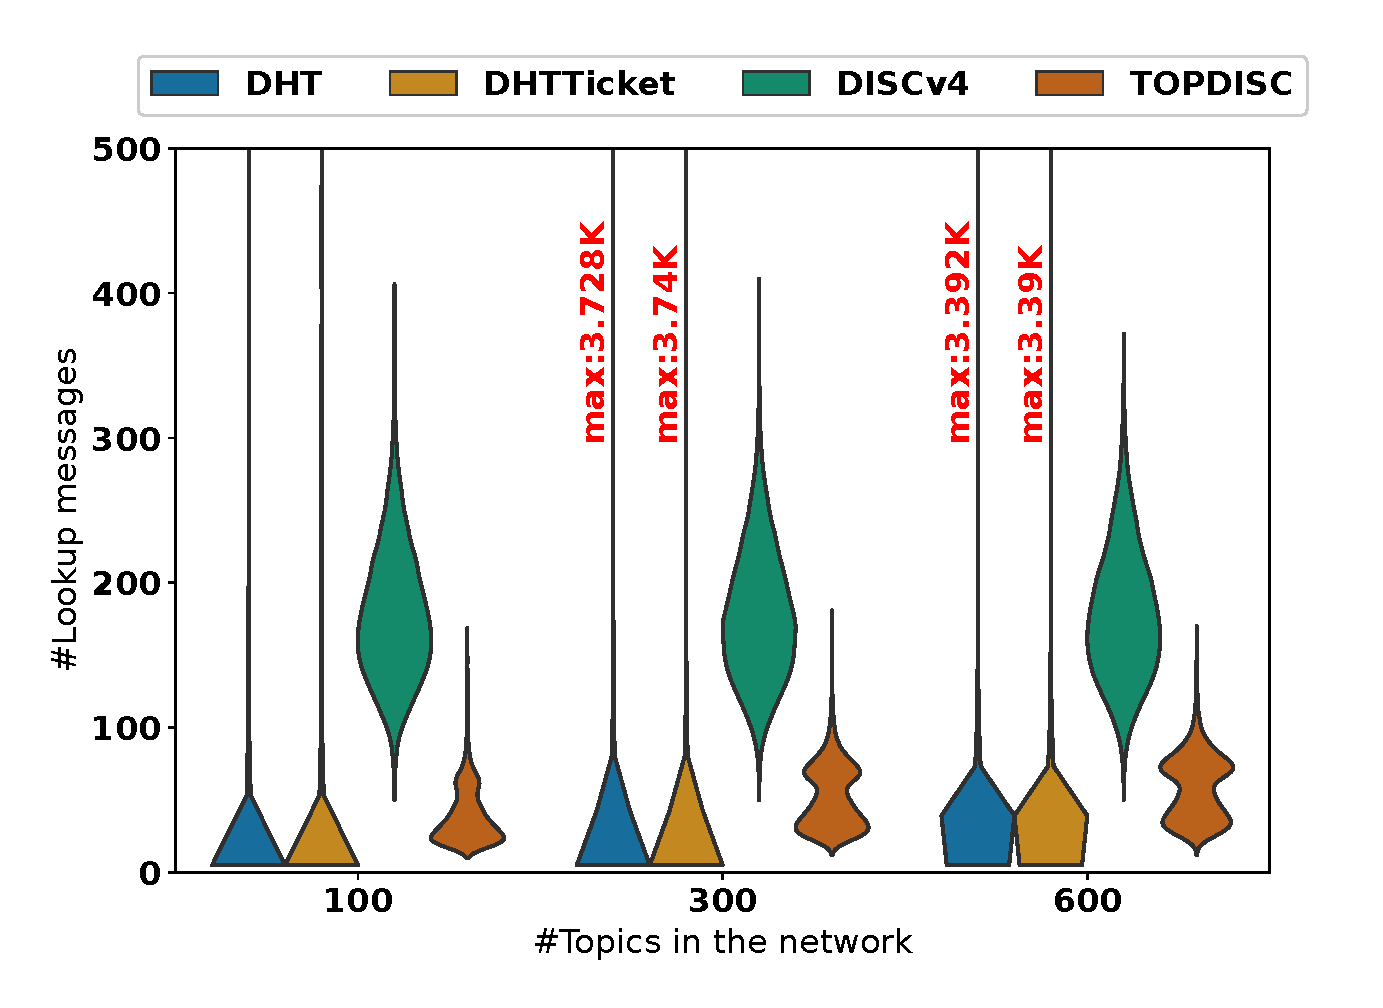
\includegraphics[width=\linewidth]{results/efficiency/violin_topic_lookupMsgs.eps}
\caption{Y-axis: Distribution of lookup messages received by peers for varying number of topics for the simulation time.}
\label{fig:lookupMsgPerTopic}
\end{figure}

\begin{figure}[!h]
\centering
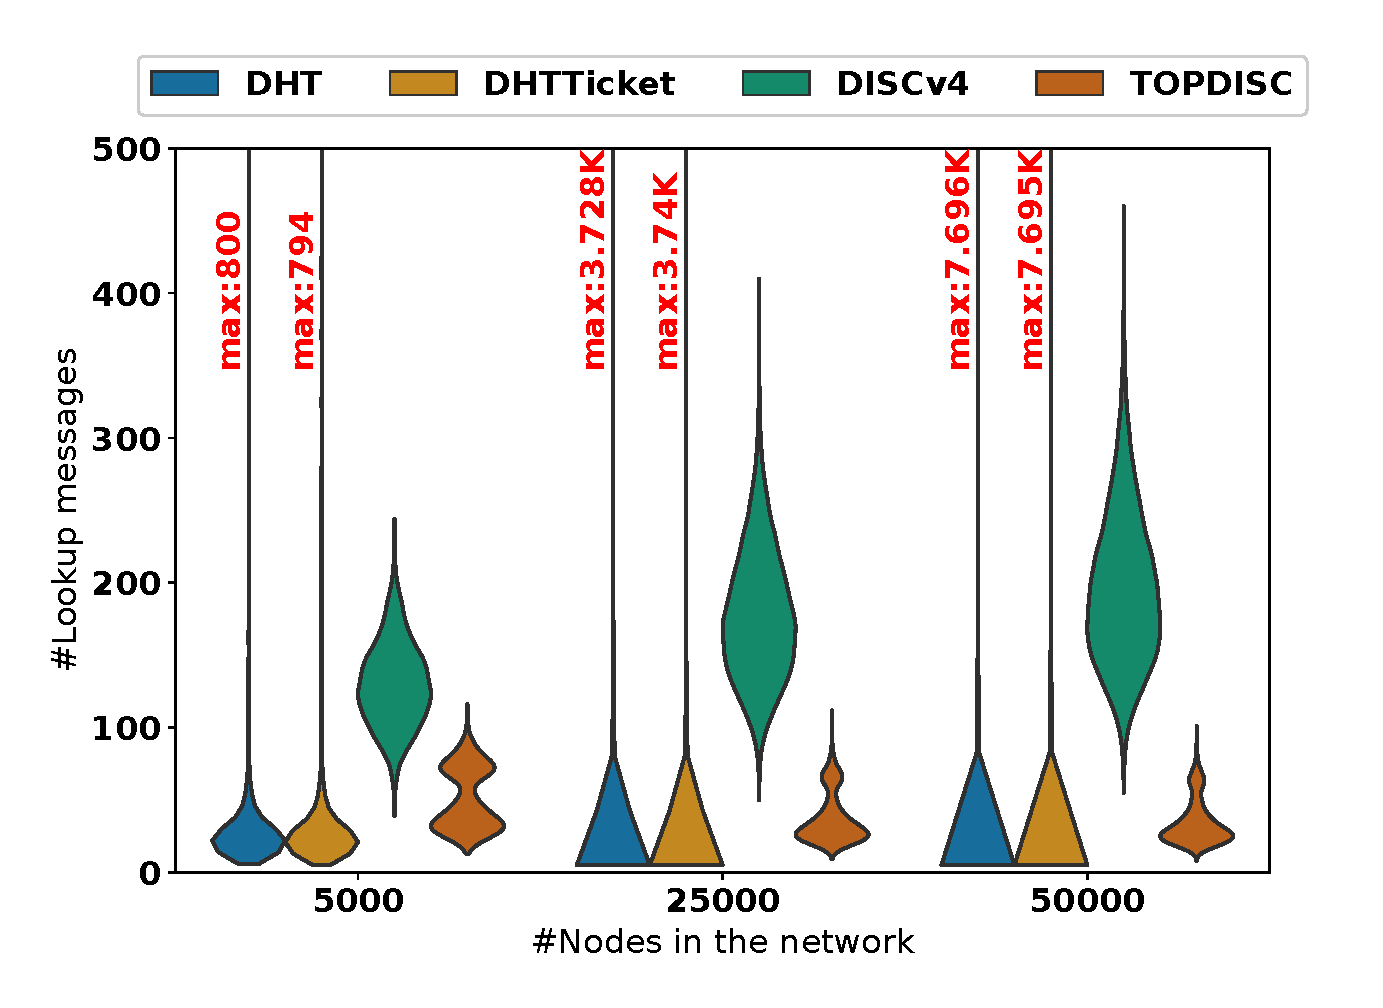
\includegraphics[width=\linewidth]{results/efficiency/violin_size_lookupMsgs.eps}
\caption{Y-axis: Distribution of lookup messages received by peers for different network size for the simulation time.}
\label{fig:lookupMsgPerSize}
\end{figure}

In~\Cref{fig:lookupMsgPerTopic}~and~\Cref{fig:lookupMsgPerSize}, we observe the number of messages related to the lookup process, \ie topic queries and replies for \sysname, \altname and \altnameticket, and kademlia find/response messages for \discv. We evaluated using  different network sizes and different number of topics in the network. 
There is a single lookup in the simulation per node, and the $N_\textit{lookup}$ parameter used is equal to 30.  Therefore nodes stop the lookup process when found 30 different nodes in the network for the intended topic.
In the figures we can observe there is a big different between topic-aware protocols (\sysname, \altname and \altnameticket) and \discv. 

\sr{why there is an increase for \discv with the number of nodes in the simulation and not the number of topics??? shouldn't be the opposite? I guess is because even if there are topics with less nodes there is just a single lookup with the same nodes contacted}
\sr{why the peak is bigger for DHT for 600 than 300? Is it because of topic hash ids colliding?}

\begin{figure}[!h]
\centering
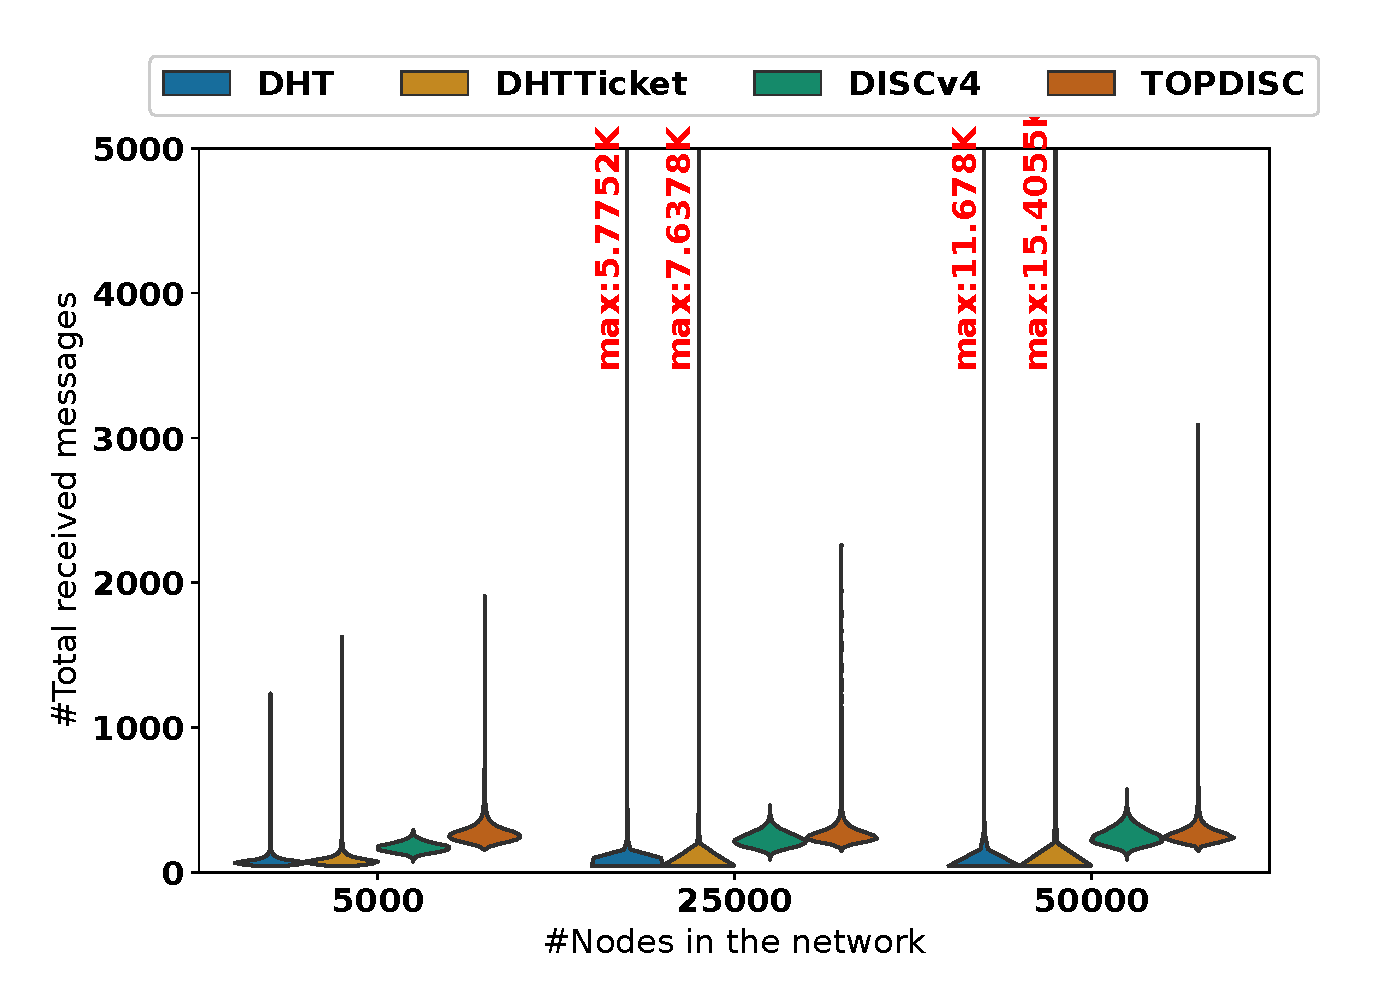
\includegraphics[width=\linewidth]{results/efficiency/violin_size_totalMsg.eps}
\caption{Y-axis: Distribution of discovery related (including registration and lookup) messages received by peers for different network size during a single advertisement period.}
\label{fig:msgsPerSize}
\end{figure}

\begin{figure}
\centering
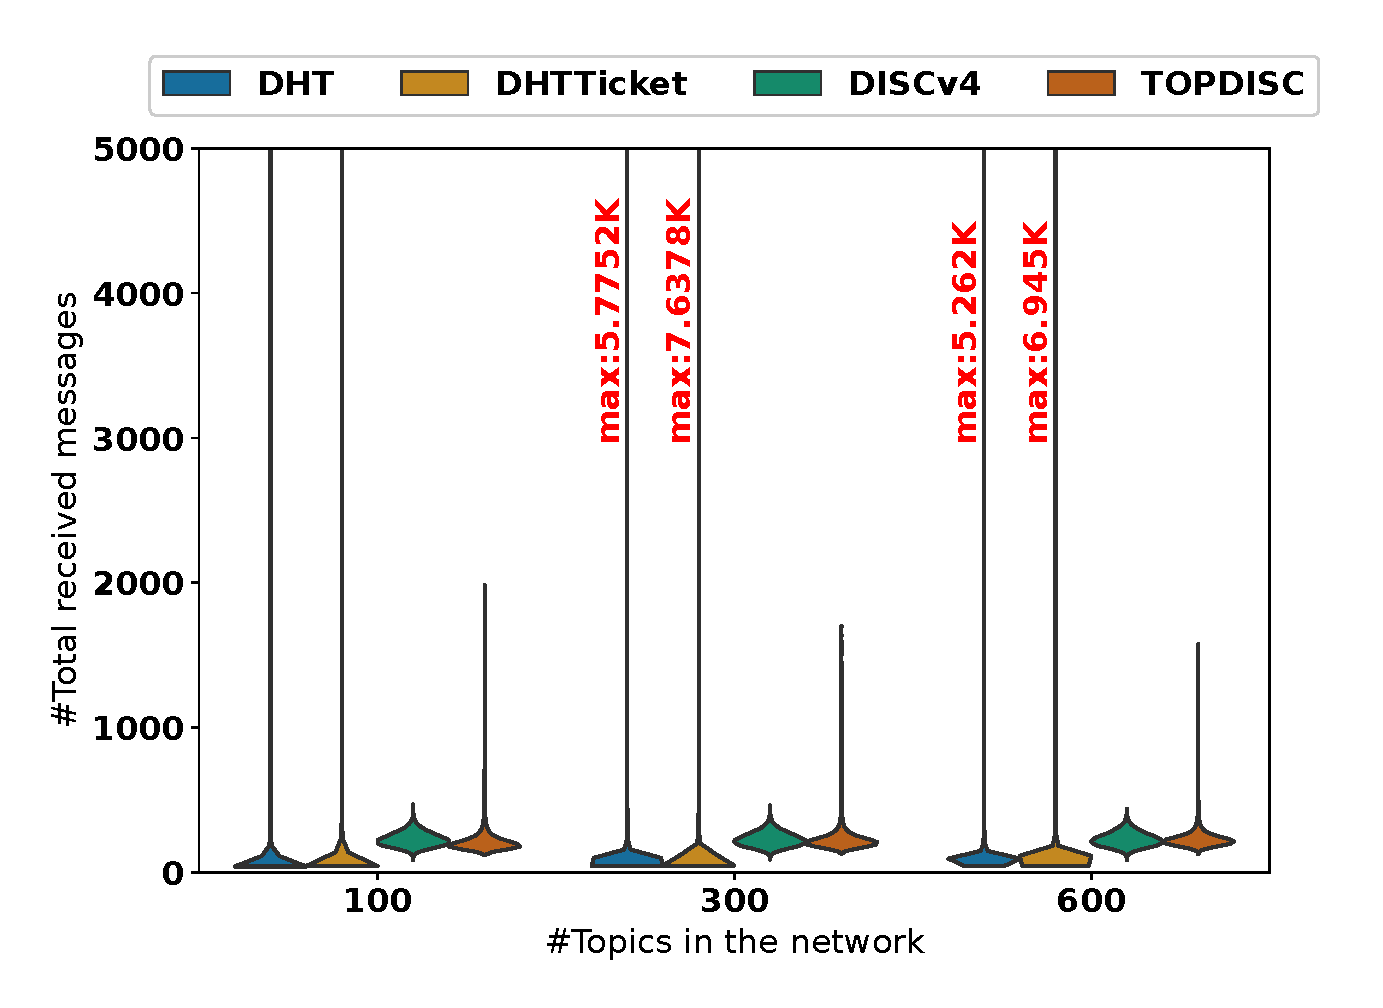
\includegraphics[width=\linewidth]{results/efficiency/violin_topic_totalMsg.eps}
\caption{Y-axis: Distribution of discovery related (including registration and lookup) messages received by peers for different number of topics during a single advertisement period.}
\label{fig:msgsPerTopic}
\end{figure}

In~\Cref{fig:msgsPerSize}~and~\Cref{fig:msgsPerTopic}, we observe the total number of messages during the simulation but normalised per advertisement period. 
Therefore in the figures, it is shown the messages related to a single lookup per node and a single registration process per node before advertisements start to expire and need to be refreshed.
This the overall overhead registered per node in the network.
We can observe that \altname protocols does not scale with the increase of nodes in the network. 
Nodes that are close to a topic hash receive most of the traffic and there is a linear increase with the number of nodes in the network. 
\discv protocol has a better distribution of the load between nodes since its behaviour is completely random. However, the average load in nodes is the highest one because of the overhead caused by not being able to find nodes for specific topics, increasing the overhead during lookup.
\sysname in comparison, provides lower overhead than the other protocols.

%%%%%%%%%%%%%%%%%%%%%%%%%%%%%%%%%%%%%%%%%%%%%%%%%%%%%%%%%%%
\subsection{Lookup performance}

\begin{figure}[!h]
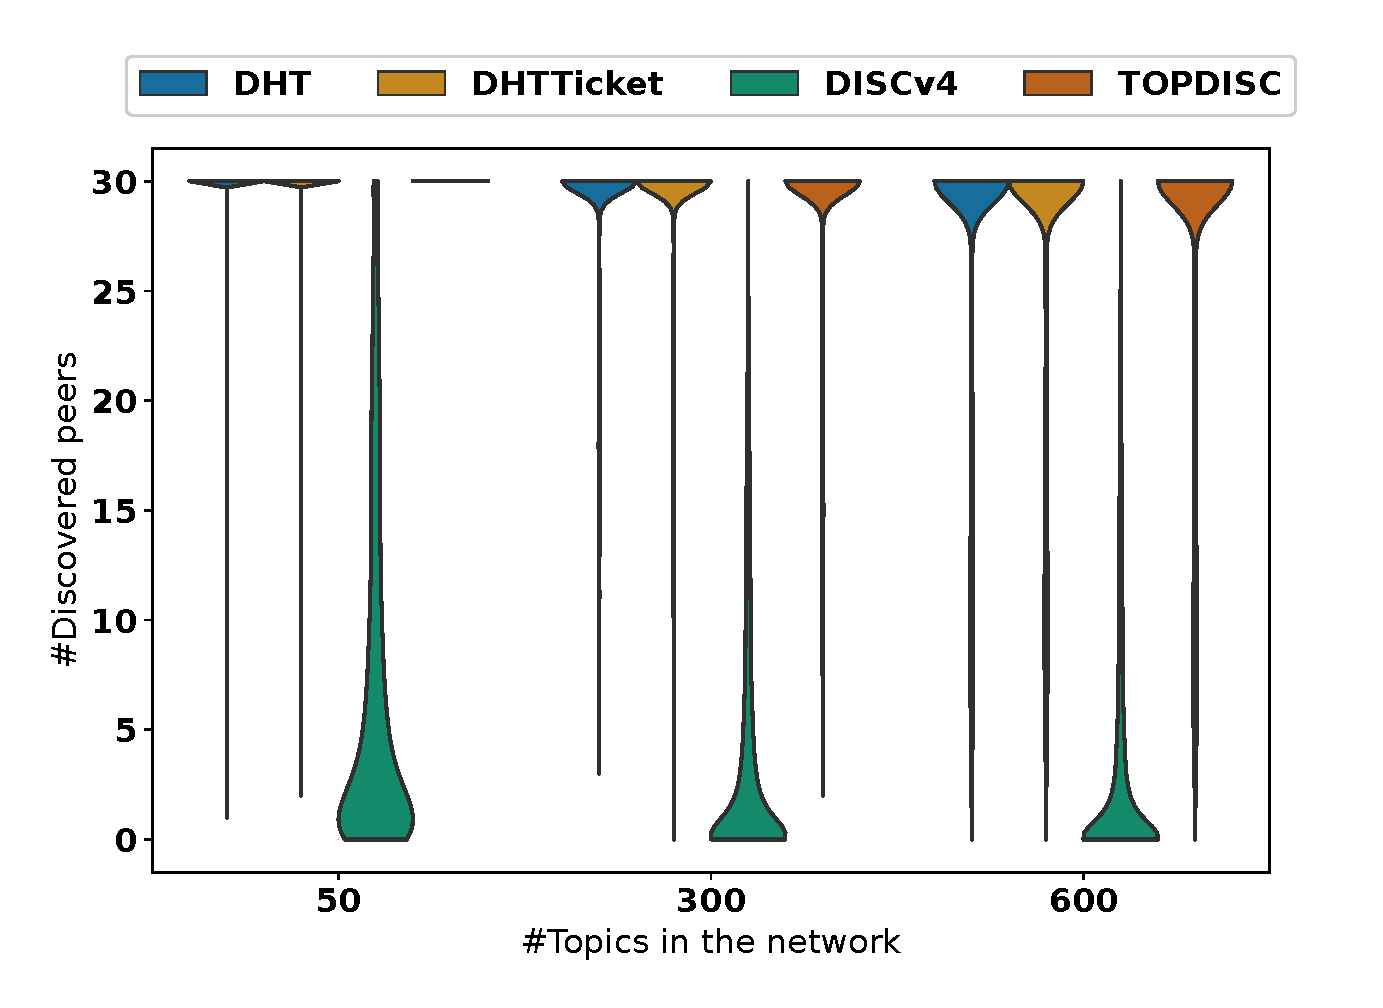
\includegraphics[width=\linewidth]{results/efficiency/violin_topic_discovered.eps}
\caption{Y-axis: Distribution of the number of peers discovered during lookup operation for different number of topics.}
\label{fig:discoveredPerTopic}
\end{figure}

\Cref{fig:discoveredPerTopic} presents the number of peers discovered during a single lookup operation with increasing number of topics in the network. The discovery becomes more difficult, as the number of topics grows.  \discv achieves a much lower number of discovered peers per operation, while \sysname and DHT-based solution efficiently discover the required amount of nodes. The rare cases where \sysname and DHT-based solution do not discover the required amount of peers are caused by small networks that consist of less than 30 nodes. 

\michal{regarding \Cref{fig:discoveredPerTopic}, it seems that for 300 and 600 topics, we discover slightly less peers on average than the DHT solutions. Why is that? Those results should be for the same topic distributions across protocols, right?}
\sergi{I think is normal and is caused by the fact that dht is going straight to nodes with most of the registrations so, specially with topics with very few nodes, they can find nodes faster, but with the tradeoff of being eclipsed very easy.}

\begin{figure}[!h]
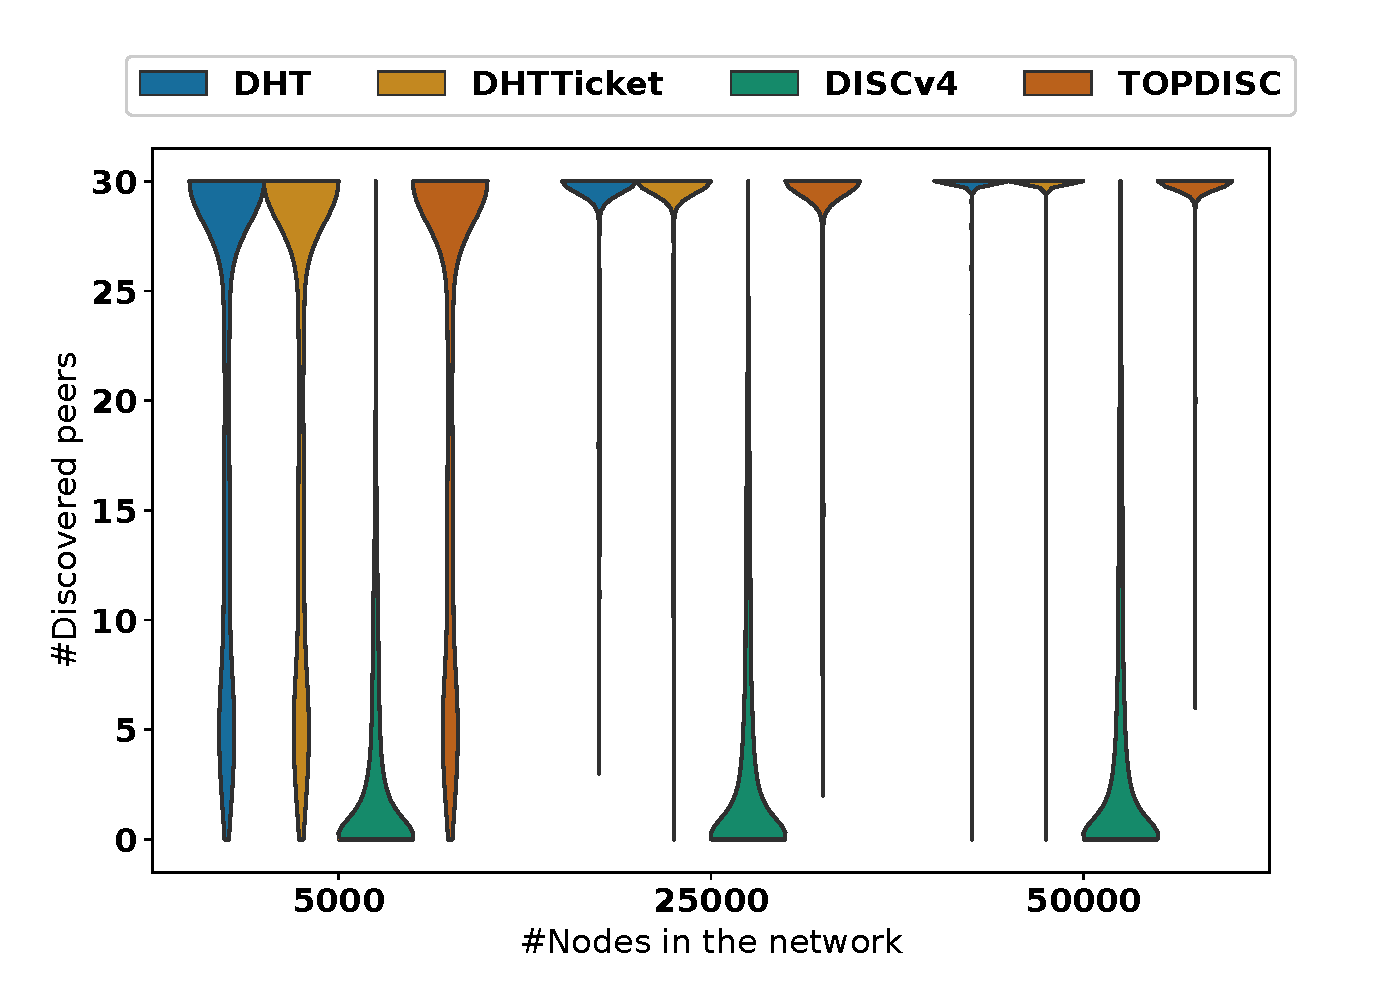
\includegraphics[width=\linewidth]{results/efficiency/violin_size_discovered.eps}
\caption{Y-axis: Distribution of the number of peers discovered during lookup operation for different network size.}
\label{fig:discoveredPerSize}
\end{figure}

\Cref{fig:discoveredPerSize} presents the number of peers discovered during a single lookup operation with increasing size of the network. With a fixed amount of topics, each application-specific network grows and for all the protocols, it is easier to find the required amount of nodes. However, discv4 suffers from poor performance for all the investigated network sizes. 

\begin{figure}
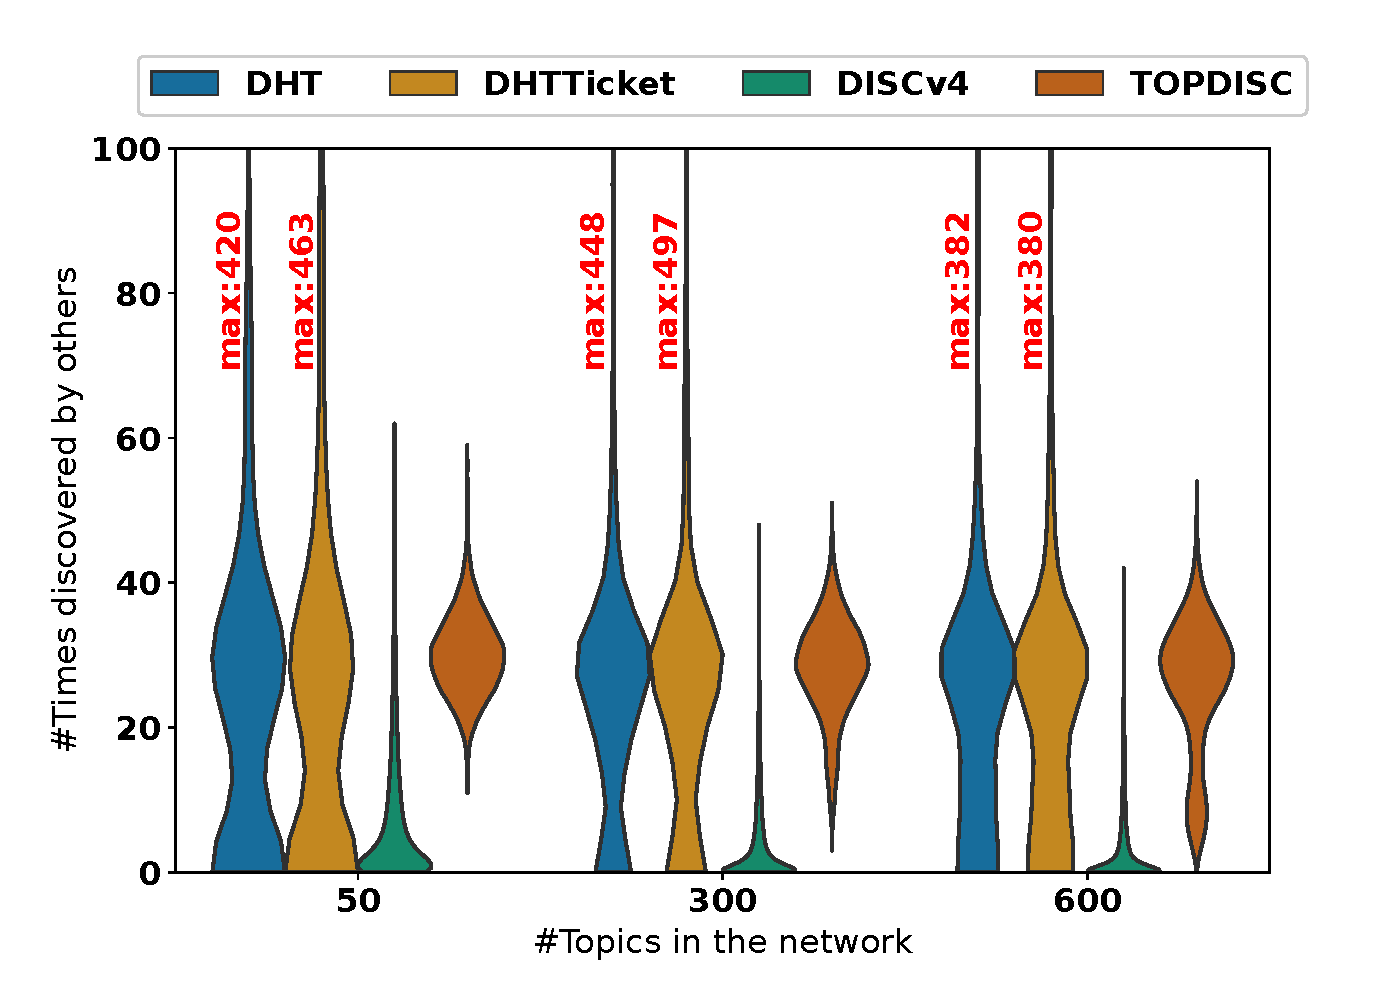
\includegraphics[width=\linewidth]{results/efficiency/violin_topic_wasDiscovered.eps}
\caption{Y-axis: Distribution of the number of times a peer is discovered by others for number of topics in the network for the simulation time.}
\label{fig:discoveredByPerTopic}
\end{figure}

\begin{figure}[!h]
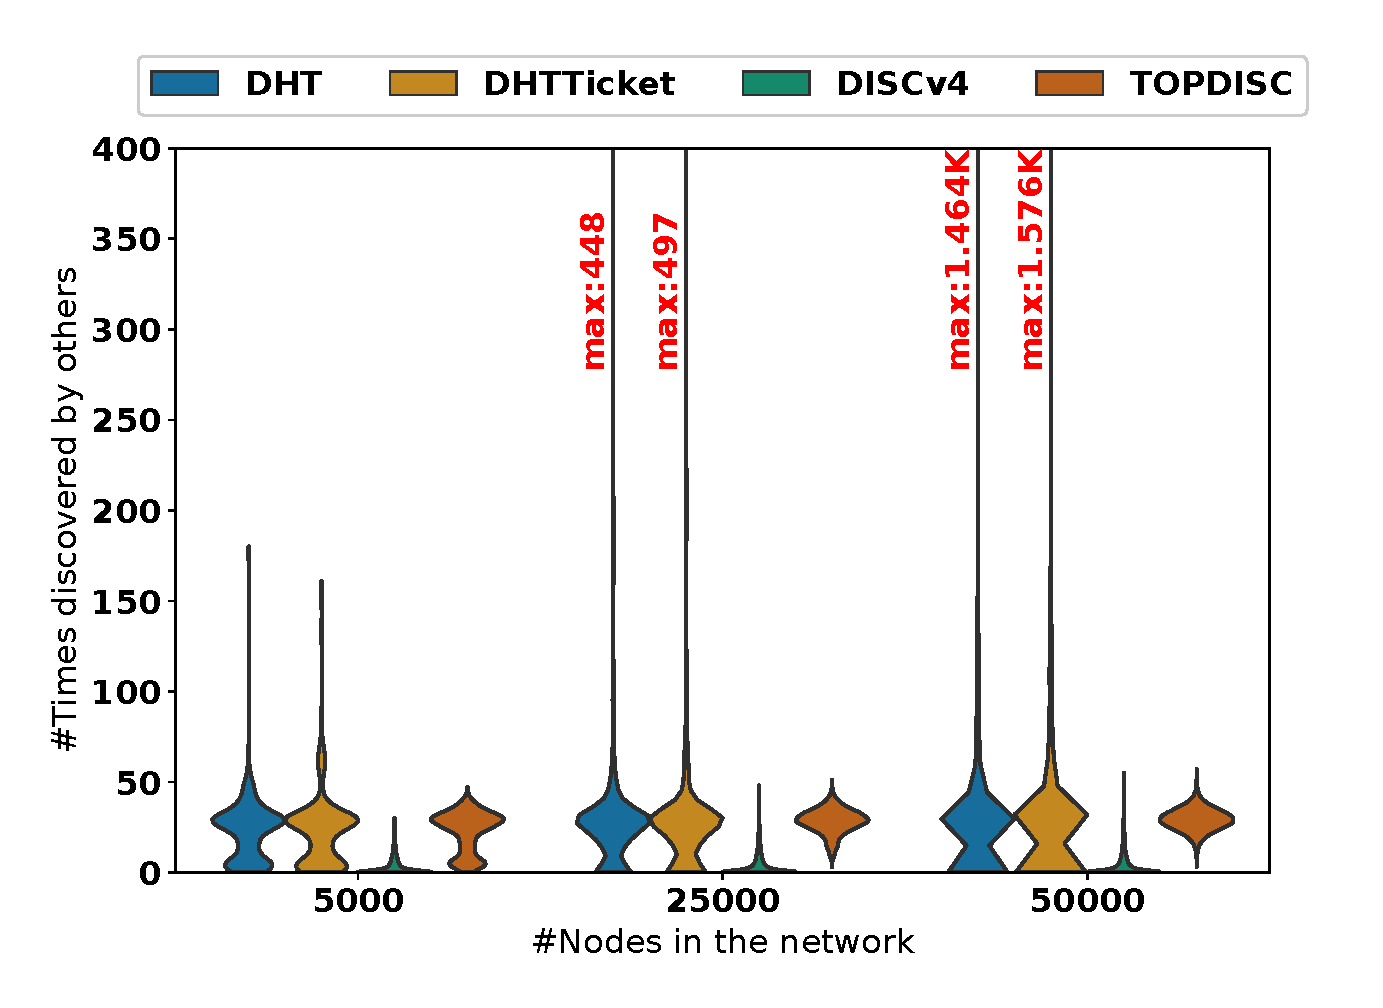
\includegraphics[width=\linewidth]{results/efficiency/violin_size_wasDiscovered.eps}
\caption{Y-axis: Distribution of the number of times a peer is discovered by others for different network size for the simulation time.}
\label{fig:efficiency_size}
\end{figure}

\subsection{Security}
%We evaluate \sysname resistance to two groups of malicious attacks:
%\begin{itemize}
%    \item \textbf{Eclipse Attack} - the attacker tries to make a target node discover and connect to peers under the attacker's control. The attack succeeds when all the inbound and outbound connections of the target node are established with malicious peers. 
%    \item \textbf{Denial of Service (DoS)} - the attacker tries to disturb protocol operations. The attack succeeds when service discovery is made impossible or significantly delayed for a group of benign nodes.  
%\end{itemize}
%The attacker may use a large but finite number of malicious nodes. Both attacks may target a single node or a group of nodes (\eg nodes participating in a specific application). 

%\para{Eclipse Attack}

\para{Eclipse Attack}
We implemented and evaluated \sysname resistance against a hybrid eclipse attack targeted to a specific topic,  that  tries to make a searcher node discover and connect to peers under the attacker's control.  
The attacker may be able to generate a large but finite number of Sybil nodes,  with limited network resources (\ie limited IP addresses used by the Sybil nodes pool used in the attack).
The attack succeeds when all the inbound and outbound connections of the target node are established with malicious peers.  The attack consists of the following:
\begin{itemize}
    \item \textbf{Registration spam} - the attacker targets a registrars and sends a large number of registrations requests. If successful, the attacker exhaust registrar's resources and prevent benign nodes from registering. 
%    \item \textbf{Malicious registrar} - the attacker deploys its nodes playing the role of registrars that \textit{(i)} return maximum waiting times when asked for a ticket, \textit{(ii)} return an empty set when asked about a topic. If successful, the attacker prevents benign advertisers from registering \textit{(i)} and prevents benign searchers from discovering their peers \textit{(ii)}. 
	\item \textbf{Malicious registrar} - the attacker deploys its nodes playing the role of registrars that only malicious sybils with the objective of preventing benign searchers from discovering valid peers and eclipsing all its connections.  We consider a coordinated eclipsing attack and any malicious registrar replies with a subset of the identifiers of the Sybil nodes controlled by the attacker.
\end{itemize}

We evaluated the resistance against eclipse attacks using the same default parameters used in the performance evaluation, that is 25000 nodes in the simulation and 300 topics by default, distributed using zipf function of exponent 1.0.  The simulation runs for 1 hour and there is a single lookup per node for the topic it participates.
Nodes get eclipsed when all nodes discovered during a lookup are malicious nodes controlled by the attacker, and therefore they only can connect to the attacker and get the view of the network from the attacker only. 

In the following figures we show violin plots representing the number of malicious nodes returned per lookup using different parameters for the same protocols evaluated in the performance simulations.  On top of each violin plot we specify the percentage of nodes eclipsed after a lookup (\ie percentage of lookups where all nodes returned are malicious nodes).
We evaluated the eclipse attacks targeting two specific topis, the most popular topic and a low popularity topic.
The most popular topic has 3978 nodes registering for this topic and the low popularity has only 33 nodes.
We evaluated the attacks for the most popular and least popular 

\sr{TODO: show protocols in the same order for all figures. redo all figures to fix it and fix also max values text}

\begin{figure}[!h]
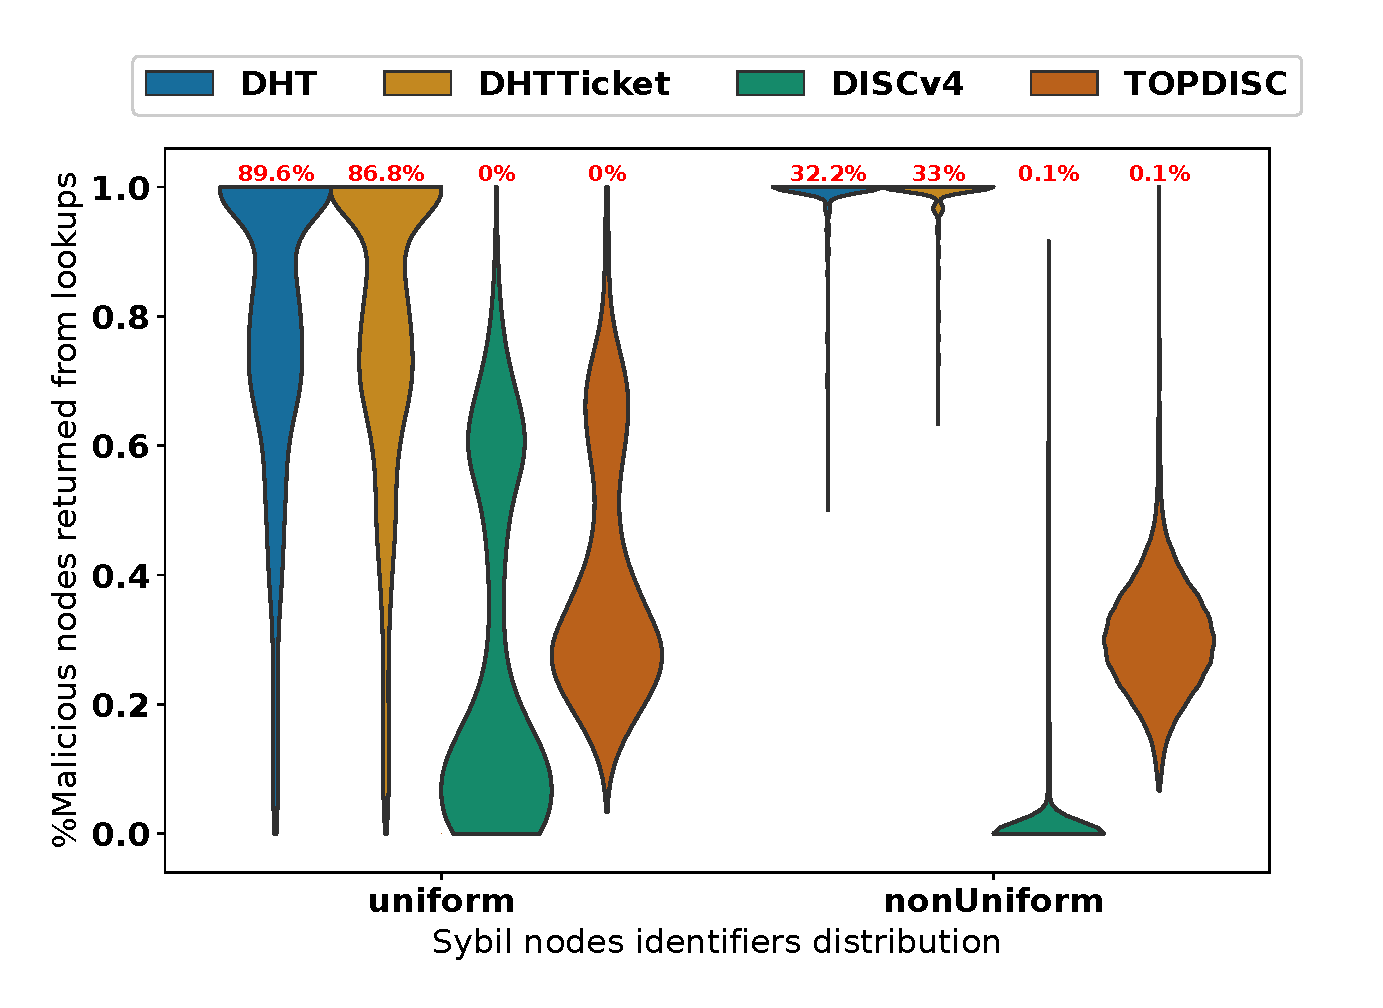
\includegraphics[width=\linewidth]{results/security/violin_idDistribution_percentageMaliciousDiscovered_t0.eps}
\caption{Y-axis: Malicious nodes discovered and percentage eclipsed nodes using uniform distributed sybil identities vs generating node ids close to topic id,   when attacking the most popular topic (3978 nodes).}
\label{fig:eclipse_distribution_t0}
\end{figure}

\sr{TODO:fix fig \ref{fig:eclipse_distribution_t0} x axis, labels are wrong.}

In Figure~\ref{fig:eclipse_distribution_t0} we show the malicious nodes discovered for all lookups for all protocols using different distribution of the identifiers of the malicious nodes,  when attacking the most popular topic (with 3978 nodes).  In the first option, the malicious nodes ids are artificially generated with a small distance to the topic hash id.  In the second option, malicious nodes identifiers are uniformly distributed.  In the figure we can observe that for \altname and \altnameticket the percentage of eclipses are superior to 80\% because most of the nodes close to topics identifiers are nodes controlled by the attacker.  
For \altname and \altnameticket, the lookup process is similar to Kademlia lookup process and,  placing all malicious nodes close the topic hash,  it makes very likely to query only malicious nodes during the process, since it only queries the closest known nodes to the topic identifier.
When attackers are uniformly distributed in the network, eclipses are reduced to close to 32.9\% and 33.7\% respectively.
Even though it is much less likely to hit malicious nodes during the lookup in this case (remember the default number of malicious are 1000 -4\% of the network-),  when hitting a malicious nodes, the nodes returned by them are used to continue the  query and it may happen it continues querying malicious nodes only during the process.
When a low popularity topic is attacked (with only 33 nodes),  as shown in Figure~\ref{fig:eclipse_distribution_t299},  for  \altname and \altnameticket the eclipses are even higher, reaching a 100\% of eclipses when placing malicious nodes close to the topic id, and reaching a 78.8\% and 90.9\% when distributing malicious nodes uniformly.  
Remember the number of attackers is 1000,  against the 33 valid nodes.

For \discv,  the number of eclipses reach is 0\% for the most popular topic when attackers are placed close to the topic hash.  When Sybil nodes are uniformly distributed the number of malicious nodes returned increases,  but to a very low 0.1\%.
This is caused by the fact that \discv does not target lookups to any specific identifier,  but completely random identifiers,  so it is very difficult for the attackers to place Sybil nodes where they will be queried.  Moreover it is difficult by the attackers to send identifiers where the lookup process will be likely to continue to,  because in the FIND node for the Ethereum DHT the lookup identifier is not disclosed,  but only the distance to it.
The number of eclipses reach 12.1.\% for the least popular topic when attackers are placed close to the topic hash.  When Sybil nodes are uniformly distributed the number of malicious nodes returned increases,  however the eclipses  reach a 78.8\%.
The resistance of \discv to Sybil attacks is obtained with the important trade-off of very low efficiency when finding nodes for specific topics, specially for low popular topics.  It is very likely that, when doing lookups using \discv for very low popular topics, no nodes are found or just a few of them.   This means when hitting a malicious node during lookup,  it is likely with a single query to a malicious node, the node querying will be eclipsed.

For \sysname, the number of eclipses are very low for the most popular topic. 
The eclipses are 0\% when Sybil nodes are placed close to topic id and 0.5\% when are uniformly distributed, with similar distribution to the malicious nodes returned compared with \discv.
However when attacking the least popular topic the eclipses increase to 78.8\% for both cases.
This is due to the very low number of valid nodes (33),  that will be more difficult to find than the attackers (1000 nodes, reusing 100 IP addresses).  
But event the high number of attackers in almost half the cases valid nodes are also found along the evil nodes.
Remember that Sybil nodes are completely valid nodes from a network discovery point of view when using different network addresses.

\begin{figure}[!h]
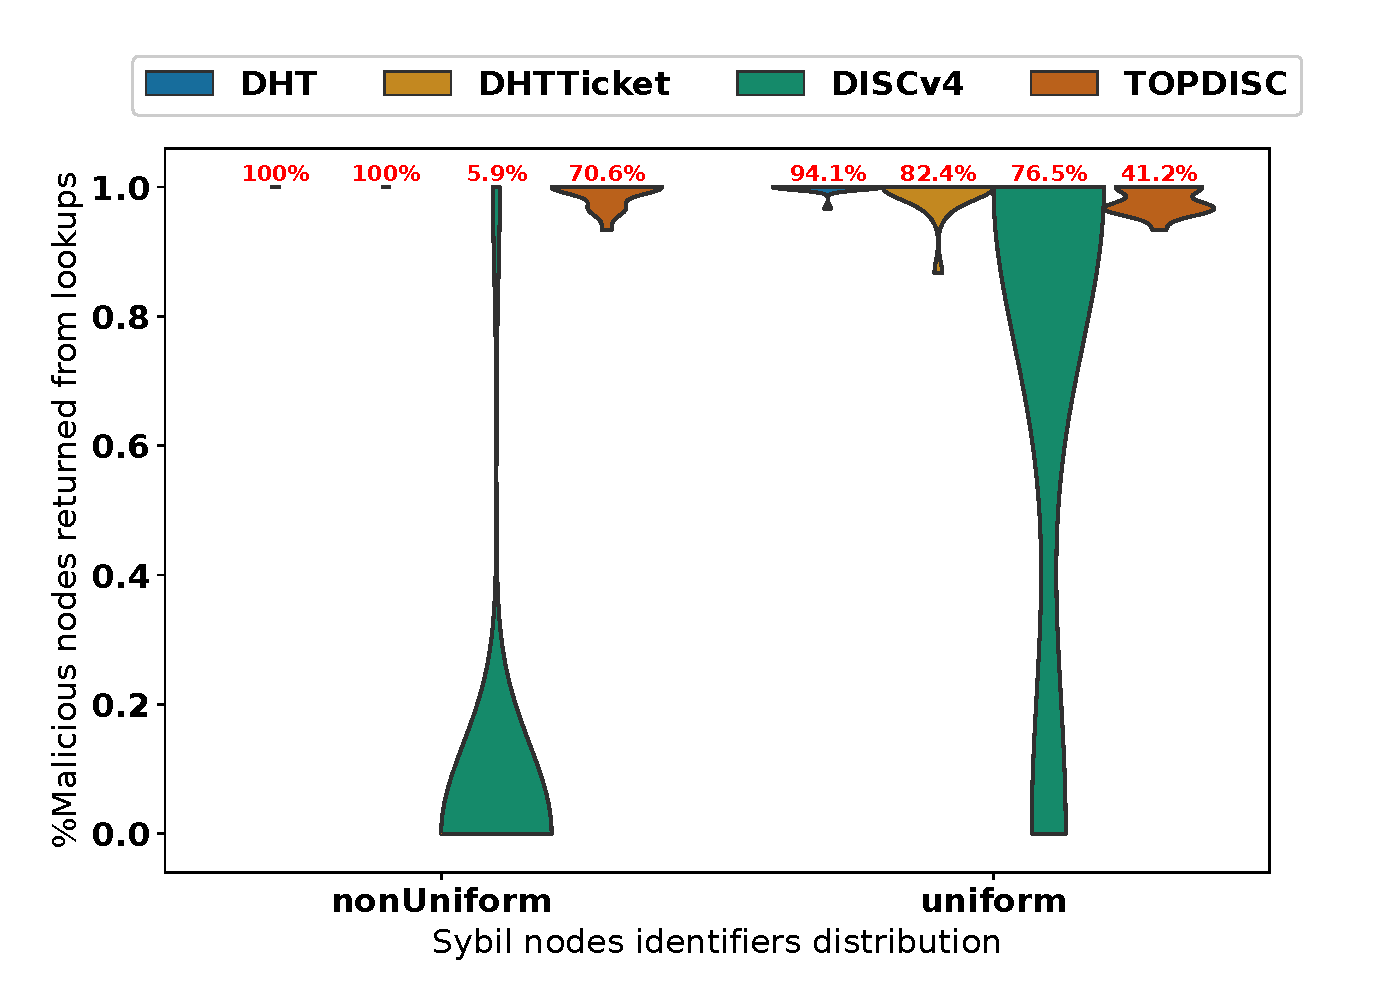
\includegraphics[width=\linewidth]{results/security/violin_idDistribution_percentageMaliciousDiscovered_t299.eps}
\caption{Y-axis: Malicious nodes discovered and percentage eclipsed nodes using uniform distributed sybil identities vs generating node ids close to topic id,   when attacking the low popularity topic (33 nodes).}
\label{fig:eclipse_distribution_t299}
\end{figure}

\sr{replace x axis for \ref{fig:eclipse_evil_t0}}

In Figure~\ref{fig:eclipse_evil_t0} we show the malicious nodes discovered for all lookups for all protocols, using different number of Sybil nodes in the network,  when attacking the most popular topic,  and in Figure~\ref{fig:eclipse_evil_t299} we show the malicious nodes discovered for the least popular topic.  In both figures attackers identifiers are generated uniformly and attackers use a pool of 100 IP addresses. 
In Figure~\ref{fig:eclipse_evil_t0}, we observe \discv is the protocol with the lowest number of eclipses and with the best distribution of malicious nodes returned during lookups.  However \sysname performs very close to \discv, having only 0.2\% of eclipses when there are 1000 attackers in the network.
\altname and \altnameticket has the worst performance,  having 47.7\% and 48.4\% of eclipses when when there are 2500 attackers.
In Figure~\ref{fig:eclipse_evil_t299}, when attacking least popular topic, we observe \sysname is the most resistant to eclipsing.
This is because it is the protocol that is able to discover more nodes with a higher diversity and is the protocol that will find easier the any of the few valid nodes in the network, and therefore it will be not eclipsed.
 
\begin{figure}[!h]
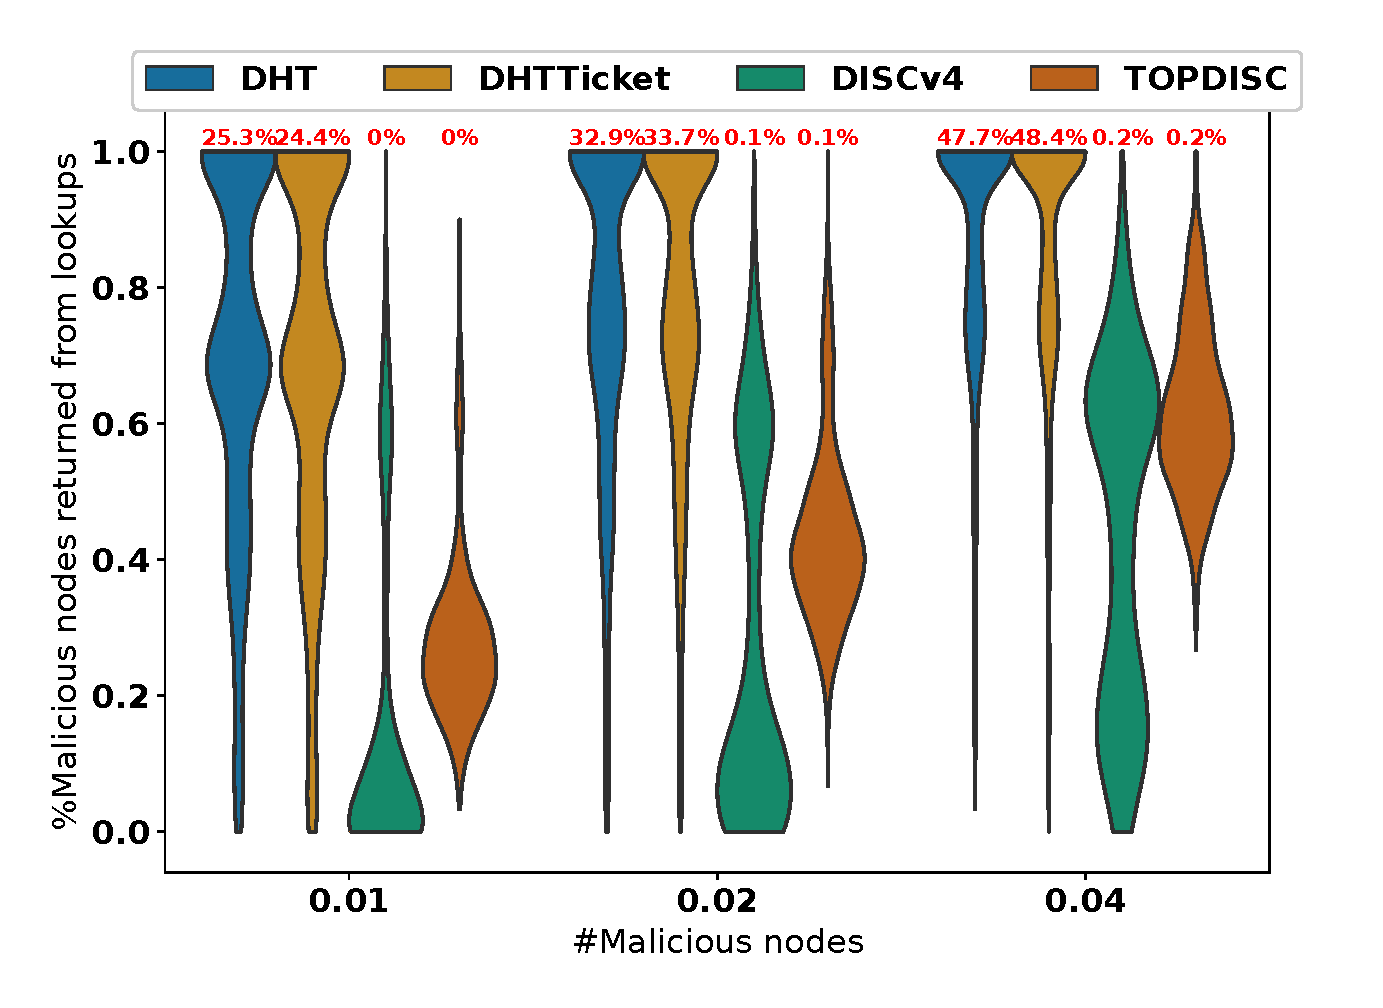
\includegraphics[width=\linewidth]{results/security/violin_percentEvil_percentageMaliciousDiscovered_t0.eps}
\caption{Y-axis: Malicious nodes discovered and percentage eclipsed nodes for different number of sybil nodes used in the attack,  when attacking the most popular topic (3978 nodes).}
\label{fig:eclipse_evil_t0}
\end{figure}

\begin{figure}[!h]
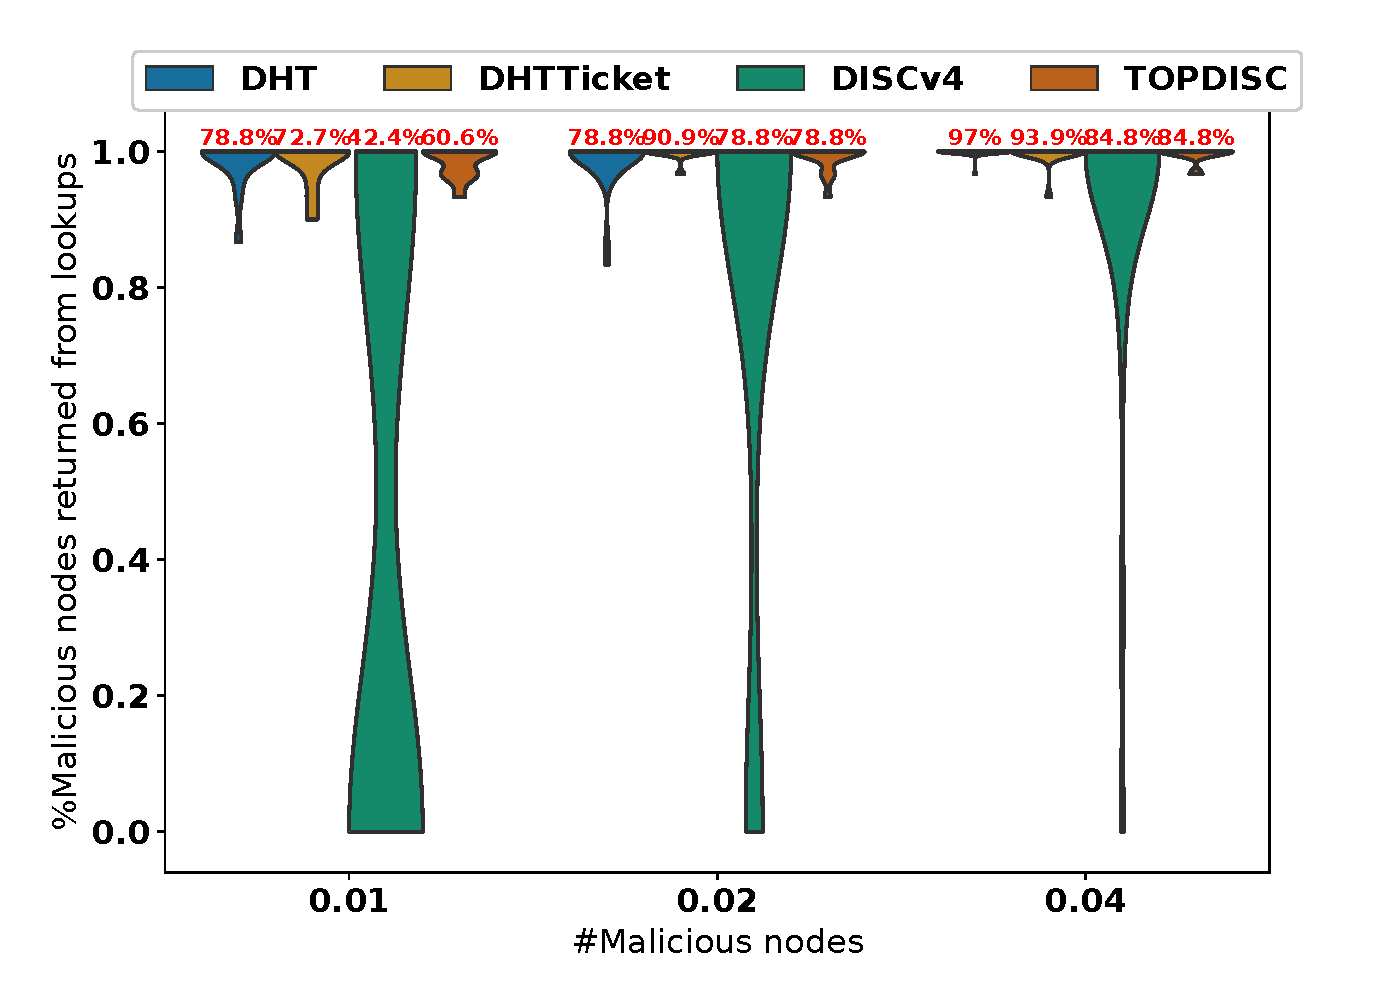
\includegraphics[width=\linewidth]{results/security/violin_percentEvil_percentageMaliciousDiscovered_t299.eps}
\caption{Y-axis: Malicious nodes discovered and percentage eclipsed nodes for different number of sybil nodes used in the attack,  when attacking the low popularity topic (33 nodes).}
\label{fig:eclipse_evil_t299}
\end{figure}


In Figure~\ref{fig:eclipse_sybil_t0} we show the malicious nodes discovered for different number of IP addresses available to the attacker,  when attacking the most popular topic,  and in Figure~\ref{fig:eclipse_sybil_t299} we show the malicious nodes discovered when attacking the least popular topic.
In this case we observe the same results than for the default values. 
\sysname is very close to \discv performance with eclipses closes to 0\% for the most popular topic, and \altname and \altnameticket is close to 33\% eclipses in all cases.
When attacking the low popularity topic,  nodes eclipsed are very similar but having a slight better performance \discv and \sysname.
There is not appreciated in the results any effect of increasing the number of IPs used by the attackers for any of the protocols.
This is caused by the fact that what is more important for the eclipses is whether you hit a malicious node during the lookup process rather than the registrations attackers are able to place in other nodes.

\begin{figure}[!h]
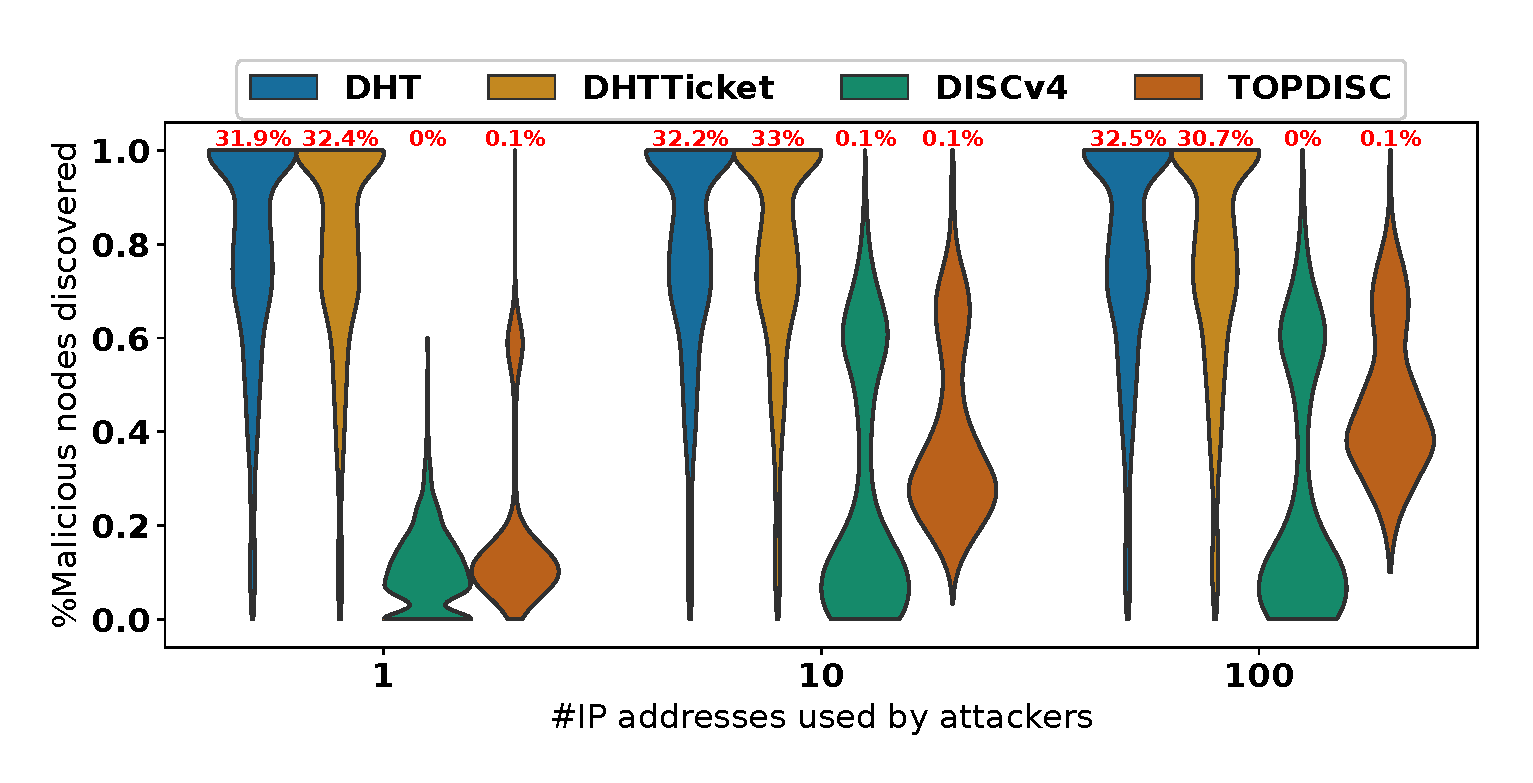
\includegraphics[width=\linewidth]{results/security/violin_sybilSize_percentageMaliciousDiscovered_t0.eps}
\caption{Y-axis: Malicious nodes discovered and percentage eclipsed nodes for different number IP addresses used in the attack,  when attacking the most popular topic (3978 nodes).}
\label{fig:eclipse_sybil_t0}
\end{figure}



\begin{figure}[!h]
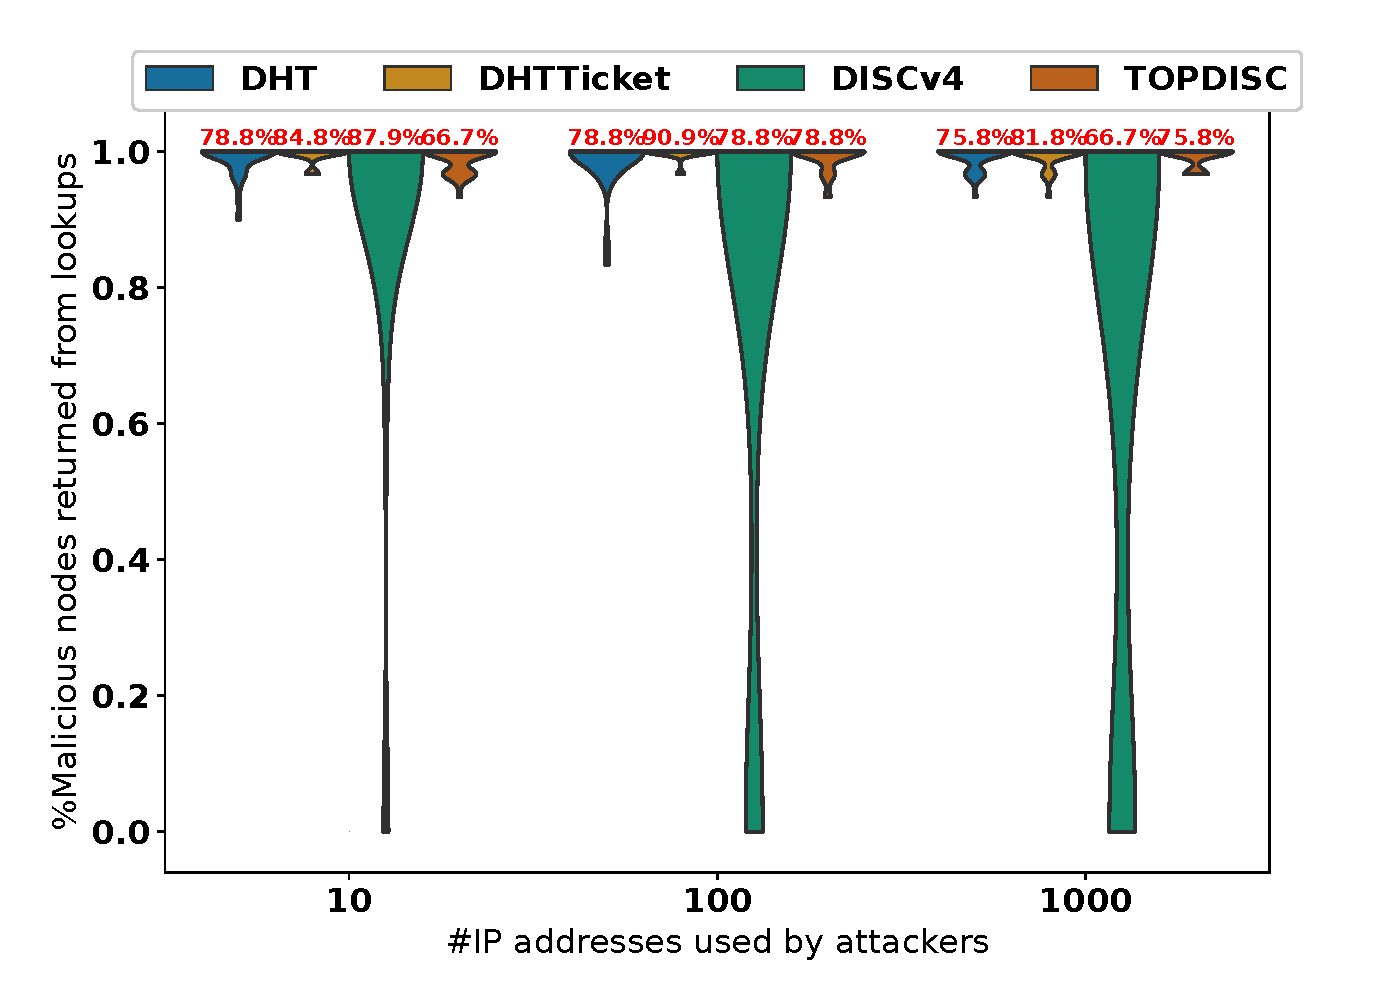
\includegraphics[width=\linewidth]{results/security/violin_sybilSize_percentageMaliciousDiscovered_t299.eps}
\caption{Y-axis: Malicious nodes discovered and percentage eclipsed nodes for different number IP addresses used in the attack,  when attacking the least popular topic (33 nodes).}
\label{fig:eclipse_sybil_t299}
\end{figure}



%\begin{figure*}[!h]
%\centering
%\subfigure[{Y-axis: Percentage eclipsed nodes using uniform distributed sybil identities vs generating node ids close to topic id}]{
%\includegraphics[width=0.31\textwidth]{results/security/%bar_idDistribution_percentageEclipsedLookups_t0.eps}
%violin_idDistribution_percentageMaliciousDiscovered_t0.eps}
%\label{fig:distribution}
%}
%\subfigure[{Y-axis: Percentage eclipsed nodes for different number of sybil nodes in the attack.}]{
%\includegraphics[width=0.31\linewidth]{results/security/%bar_percentEvil_percentageEclipsedLookups_t0.eps}
%violin_percentEvil_percentageMaliciousDiscovered_t0.eps}
%\label{fig:percentEvil}
%}
%\subfigure[{Y-axis: Percentage eclipsed nodes for different number IP addresses used in the attack.}]{
%\includegraphics[width=0.31\linewidth]{results/security/%bar_sybilSize_percentageEclipsedLookups_t0.eps}
%violin_sybilSize_percentageMaliciousDiscovered_t0.eps}
%\label{fig:sybilsize}
%}
%\caption{Resistance against eclipse attacks when attacking most popular topic (t0)} 
%\label{fig:eclipse_attack}
%\vspace{-0.05in}
%\end{figure*}
%
%\begin{figure*}[!h]
%\centering
%\subfigure[{Y-axis: Percentage eclipsed nodes using uniform distributed sybil identities vs generating node ids close to topic id}]{
%\includegraphics[width=0.31\textwidth]{results/security/%bar_idDistribution_percentageEclipsedLookups_t299.eps}
%violin_idDistribution_percentageMaliciousDiscovered_t299.eps}
%\label{fig:distribution}
%}
%\subfigure[{Y-axis: Percentage eclipsed nodes for different number of sybil nodes in the attack.}]{
%\includegraphics[width=0.31\linewidth]{results/security/%bar_percentEvil_percentageEclipsedLookups_t299.eps}
%violin_percentEvil_percentageMaliciousDiscovered_t299.eps}
%\label{fig:percentEvil}
%}
%\subfigure[{Y-axis: Percentage eclipsed nodes for different number IP addresses used in the attack.}]{
%\includegraphics[width=0.31\linewidth]{results/security/%bar_sybilSize_percentageEclipsedLookups_t299.eps}
%violin_sybilSize_percentageMaliciousDiscovered_t299.eps}
%\label{fig:sybilsize}
%}
%\caption{Resistance against eclipse attacks when attacking least popular topic (t299)} 
%\label{fig:eclipse_attack}
%\vspace{-0.05in}
%\end{figure*}
%\begin{figure}[!h]
%\includegraphics[width=\linewidth]{img/placeholder}
%\caption{Compare only against DHT here I guess? Y-axis a ratio of popular malicious and benign ads in the table for spam attack and topic-targeted attack within a single registrar. X-axis: to avoid showing different graphs for multiple malicious IPs/IDs/nodes we can have a fix ratio between them i.e., each 5 Sybils (or requests/s) have 1 IP and 2 ID, and increase this "attacker strength".} 
%\label{fig:security_spam}
%\end{figure}
%
%\begin{figure}[!h]
%\includegraphics[width=\linewidth]{img/placeholder}
%\caption{Compare only against DHT here I guess? Y-axis a  time to discovery/registration (do we care about registration if lookup works?) slowdown compared to a non-attack scenario?Do we consider different placements of Sybils here (i.e., only bucket 1? Or spread evenly across all the buckets?). X-axis: to avoid showing different graphs for multiple malicious IPs/IDs/nodes we can have a fix ratio between them i.e., each 5 Sybils have 1 IP and 2 ID, and increase this "attacker strength".} 
%\label{fig:security_spam}
%\end{figure}



\iffalse
\subsection{Performance Results}
\michal{We should group the result so that they show achievement of specific goals that we described before}

%\paragraph{Ticket registrations:
In the following we detail the performance evaluation in four different subsections.  In the first we show the registration performance.  Secondly we show the traffic load and overhead of the designed mechanism.  Then we continue with the lookup and discovery performance and we finish with the security analysis.

\subsubsection{Registration  performance}

In Figure~\ref{fig:regs} we observe the average active registrations in the system per topic with different number of nodes in the simulation,  from 500 to 10000 nodes. 
We can observe nodes for all topics are able to place a substantial amount of registrations, even the less popular topics. 
As number of nodes increase in the network, we can observe the differences between registrations per topic are reduced. 
Actually, it can be observed the most popular topic (t1) is able to place less registrations than t2. 
This is caused by the fact that with more nodes trying to register for the same topic,  waiting times increase.
If the waiting time increases over the waiting time limit (in the simulations is set to 15 min),  the node cancels the registration and tries with a different nodes.
When cancellations happen it may lead to less active registrations, because it may end up with longer registration processes.
In our simulation we observe less registrations for t1 than t2  because t1 registrations waiting time go over the waiting time limit more often.

In Figure~\ref{fig:time_reg} we observe the average time necessary for a node to place a registration,  from 500 to 10000 nodes in the simulation.
We can observe that average registration time is always below 500 seconds and this is reduced for less popular topics and smaller networks. 
This figure does not include registration times for cancelled registrations.
\sergi{I think we should include failed/uncomplete registrations in the plot}

\begin{figure}[!h]
\centering
\subfigure[{Active registrations}]{
\includegraphics[width=0.225\textwidth]{img/eval/registration_origin.eps}
\label{fig:regs}
} 
\hspace{-0.25cm}
\subfigure[{Time to register}]{
\includegraphics[width=0.225\textwidth]{img/eval/avg_time_register.eps}
\label{fig:time_reg}
}
 \caption{Ticket registrations} 
\label{fig:registrations}
\vspace{-0.15in}
\end{figure}   

%\begin{figure}[h!]
%\centering
%%\epsfig{file=imgs/eval/scen5.pdf, width=0.45\textwidth}
%\includegraphics[width=0.225\textwidth]{img/eval/registration_origin.png}
%\caption{Registrations}
%\label{fig:regs}
%\vspace{-0.15in}
%\end{figure}

%\paragraph{\bf{Network load}:}
\subsubsection{Network load}

In Figure~\ref{fig:messages}~and~\ref{fig:msg_distr} we can observe the traffic load generated in the network.
In Figure~\ref{fig:messages} we observe most of the messages are ticket requests/replies, and the subsequent registration request/replies
after receiving a ticket from a node. 
This is caused by the fact that nodes are constantly registering dynamically. 
In Figure~\ref{fig:msg_distr} the messages received distribution. 
We can observe some nodes receive much more messages.
This is caused by the bucket node distribution, where nodes with identifiers close to topic hash ids receive more initial tickets requests because there are less.
However, we observe while the number of nodes in the network is increased 20 times,  the  maximum number of messages received by some nodes does not increase in the same way,  only being twice the amount when comparing 500 with 10000 nodes,  ans with increases lower than 30\% when number of nodes are doubled.
Moreover,  we can also see the number of messages received does not exceed 10 times the average value of the messages received. 

Therefore, the system is able to scale without danger of overloading some of the nodes of the network.

\begin{figure}[!h]
\centering
\subfigure[{Number of messages}]{
\includegraphics[width=0.225\textwidth]{img/eval/message_quantity.eps} 
\label{fig:messages}
} 
\hspace{-0.25cm}
\subfigure[{Message distribution}]{
\includegraphics[width=0.225\textwidth]{img/eval/messages_received.eps} %\hspace{-1.5em}%
\label{fig:msg_distr}
}
 \caption{Traffic load} 
\label{fig:traffic}
\vspace{-0.15in}
\end{figure}   

\subsubsection{Discovery and lookup performance}

%\paragraph{\bf{Discovery performance}:}

In Figure~\ref{fig:reg_disc} and \ref{fig:timedisc} we can observe how nodes are discovered within the network.
In Figure~\ref{fig:reg_disc} we observe the percentage of the nodes in the network that are discovered and how often are discovered.
Each node in the network is represented by a circle, and the size of the circle represents the relative frequency of discoveries compared with other nodes in the network.
We can observe that for all topics the percentage of nodes discovered in the network is very close to 100\%. This means almost all nodes in the network are able to be discovered by other nodes. The number of discovered nodes is not 100\% because of the existence of turbulence (there are some nodes just joined the network and there has not been enough time yet to be discovered). In case there are a low number of nodes for a specific topic (e.g. t5 with 500 nodes network) the 100\% is reached.
We can also observe Figure~\ref{fig:reg_disc} that the discovery distribution is bounded to \hl{X} times between the most discovered and the least discovered.
We observe the dots size are very regular and despite being not completely equal the differences are not substantial. 
In Figure~\ref{fig:timedisc} we observe the time between a registration is completed and the first time the registration
is returned in a lookup.
By observing this we can see how difficult is for a node to be discovered once is able to place a registration. 
We see the average time is between 20 and 10 seconds in most of the cases, except for the least popular topic t5 which is around 50\% higher. 
We also observe the deviation is bounded at around 60 seconds, with equivalent different for t5.


\begin{figure}[!h]
\centering
\subfigure[{Advertiser discovery distribution}]{
\includegraphics[width=0.225\textwidth]{img/eval/registrant_distribution.eps} 
\label{fig:reg_disc}
} 
\hspace{-0.25cm}
\subfigure[{Time between registration and first discovery}]{
\includegraphics[width=0.225\textwidth]{img/eval/min_time_discovery.eps} %\hspace{-1.5em}%
\label{fig:timedisc}
}
 \caption{Discovery performance} 
\label{fig:discovery}
\vspace{-0.15in}
\end{figure}   


In Figure~\ref{fig:hopcount} we can observe the lookup performance of \sysname compared with Discv4 for a 5000 nodes simulation.
In the plot we show the average number of nodes discovered for each hop during a lookup per topic, taking into account that Discv4 cannot do per topic lookups,  so we discard received nodes that do not support the specific service.
In the figure we observe that for t1 the discovered nodes are higher when using Discv4, since all topics support t1 and any node discovered will be a valid node. 
However, as the popularity of the topic decreases it also does the lookup performance of Discv4,  since it is very difficult to find nodes for non-popular topics without supporting per topic lookups.
In this sense,  Discv5 lookup performance also decreases the performance with non-popular topics (simply because there are less nodes in the network) however this decrease is diminished.  Between t1 and t5 the lookup performance is decrease approximately to a 1/2th for Discv5, while when using Discv4 the lookup performance decreased to a less than a 1/10th.

%TODO add lookup description including mechanisms to avoid sybils.

\begin{figure}[h!]
\centering
%\epsfig{file=imgs/eval/scen5.pdf, width=0.45\textwidth}
\includegraphics[width=0.35\textwidth]{img/eval/lookup_hopcount_discv4.png}
\caption{Lookup performance}
\label{fig:hopcount}
\vspace{-0.15in}
\end{figure}

\subsubsection{Sybil Attacks}

In the following we show the results of the performance evaluation of the discovery service under different sybil attacks.  The attacks that we evaluated in this section are of two types and are previously described in Section~\ref{sec:overview}. 
These attacks are eclipsing  and Denial-of-service (DoS) attacks.
Eclipsing attacks goal is to generate multiple fake identities within a topic to be able to eclipse existing nodes in the network.
Eclipsing a node imply all outbound and inbound connections are established to only sybil/fake nodes controlled by an attacker.
This allows the attacker to control the view of the network of the eclipsed node and can be used to co-opt a victim's mining power and use it to attack the blockchain's consensus algorithm.
DoS attacks instead is an attack meant to hamper the good performance or even to shut down the network, making it inaccessible to its intended users.  
In our case,  the goal of DoS attacks is to difficult or to block the discovery of nodes in the network and is specially important for topic with low popularity where finding all node in the network is very important.

In the implemented topic eclipsing attack,  malicious nodes are sybil nodes that cooperate in order to eclipse other valid nodes.
Malicious and valid nodes have the same amount of bandwidth resources and malicious nodes respond to topic lookup requests and find messages with only other malicious nodes.
Malicious nodes also act as evil 'advertisers' trying to place as many registrations as possible by using bigger ticket size,  with malicious registrars attack,  where evil registrars replies with only malicious nodes when receiving a topic query.

We implemented and evaluated two kind of DoS attacks.  
The first attack consists in a topic spam attack where a big number of sybil identities generated try to register for non-existing random topics.
By registering for non-existing topics,  evil nodes try to harm valid topics registrations, overflowing topic tables.
The second DoS attack consists on generating sybil identities that keep without replying when receiving valid nodes ticket requests or return very long waiting times. 
This way an attacker can try to backlog valid nodes ticket registrations.

In Figures~\ref{fig:reg_eclipse},~\ref{fig:discoverytime_eclipse}~and~\ref{fig:lookup_eclipse} we show performance results under a
topic eclipsing attack.
We compare results for topic eclipsing attacks targeted to the most popular topic (t1) and attacks targeted to the least popular topic (t5). 
In the simulation there are 2000 nodes, all of them participating in t1 and only 218 participating in t5. 
In the simulations there are an additional 20\% (400 in total) malicious nodes that target the specific topic and the number of resources used in the attack (IP addresses) vary from 1 address to 50.

\begin{figure}[!h]
\centering
\subfigure[{Active registrations eclipse attack t1 attack}]{
\includegraphics[width=0.22\textwidth]{img/eval/attack/registration_origin_t1.eps} 
\label{fig:reg_eclipse_t1}
} 
\hspace{-0.15cm}
\subfigure[{Active registrations eclipse attack t5 attack}]{
\includegraphics[width=0.22\textwidth]{img/eval/attack/registration_origin_t5.eps} %\hspace{-1.5em}%
\label{fig:reg_eclipse_t5}
}
 \caption{Active registrations under topic eclipsing attack} 
\label{fig:reg_eclipse}
\vspace{-0.15in}
\end{figure}   

In Figure~\ref{fig:reg_eclipse_t1} we observe the active registrations in the simulation per topic, for an eclipsing attack targeted to the most popular topic (t1), including active registrations of malicious nodes.
We can observe than even though the number of malicious nodes is equivalent to 20\%, the number of active registrations is lower than that. 
As expected, as the number of IP addresses used in the attack increaseas, the number of active registrations of malicious nodes also increase, since different malicious nodes with complete different IPs can not be diffierentiated from valid nodes.
For topic 5, the most vulnerable topic for being the least popular, we can observe a similar pattern of active registrations. 
However, we observe that despite malicious nodes being more (400 nodes) than valid nodes (218 nodes), active registrations of malicious nodes is kept lower than 30\% in all cases. Similarly to t1, the active registrations increase with the higher number of IPs used in the attack, since there is no way to a totally distributed attack without reusing IP addresses.


\begin{figure}[!h]
\centering
\subfigure[{Time between registration and first discovery t1 attack}]{
\includegraphics[width=0.225\textwidth]{img/eval/attack/min_time_discovery_t1.eps} 
\label{fig:discoverytime_eclipse_t1}
} 
\hspace{-0.16cm}
\subfigure[{Time between registration and first discovery t5 attack}]{
\includegraphics[width=0.225\textwidth]{img/eval/attack/min_time_discovery_t5.eps} %\hspace{-1.5em}%
\label{fig:discoverytime_eclipse_t5}
}
 \caption{Time between registration and first discovery under topic eclipsing attack} 
\label{fig:discoverytime_eclipse}
\vspace{-0.15in}
\end{figure}   

In Figure~\ref{fig:discoverytime_eclipse} we observe the average time between a node registers for a topic successfully and the node is discovered for the first time from the placed registration.
We can observe that when a topic is under attack the time required for first time discovery increases. 
This is caused by the fact that there are much more registrations in the topic caused by the attack and also that malicious nodes discovery time is higher due to the difficulty to place registrations in nodes close to the topic hash.  
We can observe that when using more IP addresses in the attack the time required to discover a node is reduced because malicious nodes are more discovered.

\begin{figure}[!h]
\centering
\subfigure[{Lookup hopcount eclipse attack t1}]{
\includegraphics[width=0.225\textwidth]{img/eval/attack/lookup_hopcount_t1.eps} 
\label{fig:lookup_eclipse_t1}
} 
\hspace{-0.16cm}
\subfigure[{Lookup hopcount eclipse attack t5}]{
\includegraphics[width=0.225\textwidth]{img/eval/attack/lookup_hopcount_t5.eps} %\hspace{-1.5em}%
\label{fig:lookup_eclipse_t5}
}
 \caption{Lookup hopcount under topic eclipsing attack} 
\label{fig:lookup_eclipse}
\vspace{-0.15in}
\end{figure}   

\sergi{redo fig14 and fig15 figures increasing font and using eps}

In Figure~\ref{fig:lookup_eclipse} we observe the lookup hopcount in the simulation per topic,  for an eclipsing attack targeted to the most popular topic (t1) and the least popular topic (t5).
We observe that despite receiving an attack targeted at a specific topic,  the lookup performance in the network is not substantially affected by the attack.

In Figure~\ref{fig:perf_spam} we observe the performance of the topic discovery system under  the topic spam attack.
\sergi{TODO: add no sybil in the graph}
In Figure~\ref{fig:active_regs_spam} we observe the average active registrations per topic increasing the number of IP addresses used by sybil identities performing the attack.  
We observe that the number of active registrations per topic are decreased under the topic spam attack being topic 1 the most affected.
However, by observing Figure~\ref{fig:hopcount_spam} we see he lookup performance is not affected and therefore there is no substantial impact of the attack in the discovery performance of the network, concluding the system is resistant to topic spam attacks.
In Figure~\ref{fig:time_register_spam} we observe the average time required for registering for a topic,  increasing the number of Ip addresses used by sybil identities performing the attack.  
We observe again it seems there is no substantial impact of the attack to the time required to register for each topic

\sergi{add spam storage used?}

\begin{figure*}[!h]
\centering
\subfigure[{Active registrations under topic spam attack}]{
\includegraphics[width=0.275\textwidth]{img/eval/attack/registration_origin_spam.png} 
\label{fig:active_regs_spam}
} 
\hspace{-0.16cm}
\subfigure[{Time to register under topic spam attack}]{
\includegraphics[width=0.275\textwidth]{img/eval/attack/avg_time_register_spam.png} %\hspace{-1.5em}%
\label{fig:time_register_spam}
}
\hspace{-0.15in}
\subfigure[{Lookup hop count topic spam attack}]{
\includegraphics[width=0.275\textwidth]{img/eval/attack/lookup_hopcount_spam.png} %\hspace{-1.5em}%
\label{fig:hopcount_spam}
}
\caption{Performance evaluation topic spam attack} 
\label{fig:perf_spam}
\vspace{-0.15in}
\end{figure*}   

In Figure~\ref{fig:perf_dos} we observe the performance of the topic discovery system under the dos attack where registrars do not respond to advertisers trying to block active registrations.
In Figure~\ref{fig:active_regs_dos} we observe the average active registrations per topic increasing the number of sybil identites from 5\% to 20\% of the nodes in the network.
We observe that the number of registrations are affected by attackers,  being more affected for very popular topics,  but less affected low popularity topics.  However in none of the cases malicious nodes are able to block the active registrations and the reduction of the performance is lower than the number of sybils used.
In Figure~\ref{fig:time_register_dos} we observe the average time required for registering for a topic,  increasing the number of sybil identites from 5\% to 20\% of the nodes in the network.
We observe in this case it seems there is no substantial impact of the attack to the time required to register for each topic
In Figure~\ref{fig:time_discovery_dos} we observe the average time between an advertiser place a registration in a registrar and another node discovers it through the registrar,  increases the number sybils again.
We also observe there is no substantial impact of the attack, concluding the system is resistant to DoS attacks.

\begin{figure*}[!h]
\centering
\subfigure[{Active registrations under DoS attack}]{
\includegraphics[width=0.275\textwidth]{img/eval/attack/registration_origin_dos.png} 
\label{fig:active_regs_dos}
} 
\hspace{-0.16cm}
\subfigure[{Time to register under DoS attack}]{
\includegraphics[width=0.275\textwidth]{img/eval/attack/avg_time_register_dos.png} %\hspace{-1.5em}%
\label{fig:time_register_dos}
}
\label{fig:discovery_dos}
\hspace{-0.15in}
\subfigure[{Time to first discovery under DoS attack}]{
\includegraphics[width=0.275\textwidth]{img/eval/attack/min_time_discovery_dos.png} %\hspace{-1.5em}%
\label{fig:time_discovery_dos}
}
\label{fig:perf_dos}
\caption{Performance evaluation no-response DoS attack} 
\vspace{-0.15in}
\end{figure*}   

\fi
%\subsection{Testbed evaluation}
%
%"Geth"~\cite{go-ethereum} performance evaluation: \hl{TBC}.


%!TEX root = ../main.tex
%=========================================================

\vspace{-5mm}
\section{Related Work}
\label{sec:related}
\vspace{-2mm}

\mk{TODO:Mention previous work suggested by the NDSS reviewers~\cite{liu2010netfence, crowcroft2007lazy, kung2015practical}} \er{as per discussion, these should be discussed in the RW and not in the admission section.}

A decentralized service discovery system can be organized by directly storing the membership information in a DHT~\cite{can,chord,rowstron2001pastry,maymounkov2002kademlia}. 
DHT-based solutions offer fault-tolerant, scalable and efficient ways of finding nodes in large-scale networks.
However, it is difficult to guarantee the availability of published service descriptions.
If nodes close to a service hash fail, the whole sub-network becomes undiscoverable. 
While solutions such as Chord4S~\cite{chord4s} reduce this risk, the main drawback remains the vulnerability to Sybil attacks.

Other systems implement service discovery on top of publish-subscribe platforms.
However, those solutions are built directly on top of a DHT~\cite{scribe,poldercast,banno2015} (and share its weaknesses), introduce significant overhead to keep the data up to date~\cite{gossipsub}, introduce a single point of failure~\cite{dan2012centralized}, or require all nodes to be correct (\ie not byzantine)~\cite{baldoni2007tera}.

Recently, multiple service discovery protocols were implemented for the blockchain space~\cite{farmer2021decentralized, manevich2019endorsement, keizer2021flock}.
Unfortunately, these solutions are meant to work in small-scale systems~\cite{farmer2021decentralized}, or require writing to the blockchain (thus introducing significant monetary and/or computational cost)~\cite{manevich2019endorsement, keizer2021flock}. 

Multiple works proposed DHT enhancements to make it more resistant to Sybil attacks.
This can be achieved by exploiting social relations between participants operating the nodes~\cite{danezis2005sybil, danezis2009sybilinfer}, introducing some kind of Proof-of-Work~\cite{skad} or sampling participant identifiers~\cite{cholez2010efficient}.
All these solutions are difficult to implement in current P2P networks, and may have a negative impact on privacy.
An extensive number of systems have been proposed for resilient peer sampling in P2P networks~\cite{bortnikov2009brahms, jelasity2007gossip, ouguz2014stable, pigaglio2022raptee}.
While those systems are useful in some scenarios, they cannot be easily adapted to application-specific peer sampling required by the Ethereum ecosystem.

Relevant to our work, the Ethereum DHT was recently enhanced~\cite{marcus2018low, henningsen2019eclipsing} to make it more resistant to low-resource eclipse attacks at the DHT level. Those solution enable \sysname to operate, as it relies on honest participants not being fully eclipsed at the DHT level.

The enforcement of a waiting time for incoming requests to improve fairness and implement rate control has been used for preventing DDoS attacks towards centralized services or domains.
In this context, the key interest is to avoid maintaining per-client state at a server while offering priority services to clients that have waited the longest, and to adjust waiting times based on per-domain traffic and congestion.
Implementations of this idea include NetFence~\cite{liu2010netfence}, Lazy Suzan~\cite{crowcroft2007lazy} and the work of Kung \emph{et al.}~\cite{kung2015practical}.
In contrast with \sysname, however, these approaches do not focus on content (topic ads) diversity, but only use enforced waiting for rate control.
% They also do not consider a decentralized system.

%\er{Maybe discuss the byzantine-resilient peer sampling system Brahms, that also uses a blocking mechanism when more than a threshold number of view updates (pushes) are received in a certain amount of time (not sure if this is overall or for a specific node though)~\cite{}}

%There exists several protocols aimed at discovery devices providing network services for local area networks.
%For instance, the Simple Service Discovery Protocol (SSDP)~\cite{helal2002standards}, basis of the discovery protocol of Universal Plug and Play (UPnP)~\hl{missing ref}, or the DNS-based service discovery~\cite{RFC6763}, are used to advertise services that other devices provide, such as printers, webcams, HTTPS servers, and other mobile devices, usually using multicasting or broadcasting techniques.
%However for service discovery in Internet-wide environments, since it is not possible to broadcast, centralized setups are commonly used to provide service discovery with good performance.
%UDDI~\cite{zhang2002aggregate} has been recognized as the most popular discovery mechanism for Web services.

%The attack ensures that the lookup-buffer used to initiate outbound connections is filled up with adversarial nodes by placing an adversarial node to each one of the DHT buckets, requiring only 2 IPs from distinct /24 subnets to be successful.
%As a result of this paper,  Ethereum network and Geth v1.8 and v1.9 implemented new countermeasures, such as  increasing number of connections, considering all nodes of the table during lookups, or throttling the inbound connection attempt, to reduce the chance of selecting an attacker-node.
%These countermeasure have been added in our simulations for the underlying Kademlia protocol.

%In the area of avoiding Sybil and derived eclipsing attacks in peer-to-peer networks several solutions and state-of-the-art can be found in the literature.
%In~\cite{danezis2005sybil}, different strategies are devised to make DHTs resilient to malicious nodes trying to poison lookups, by routing queries in a way that minimizes trust bottlenecks, to minimize the amount of poisoned information that honest nodes receive from adversarial nodes.
%In a similar way, S/Kademlia~\cite{skad} propose new mechanisms to get resilience against common attacks by using parallel lookups over multiple disjoint paths, limiting free nodeld generation with crypto puzzles and introducing a reliable sibling broadcast.
%In ~\cite{cholez2010efficient}, the authors propose a statistical approach to detect a particular type of Sybil attack in  Kademlia DHT, where Sybil peers strategically choose IDs that are close to a target ID in the DHT ID space.

%The authors found that the expected the ID distribution of the closest nodes returned in the search results for target IDs follow a geometric distribution. Therefore, the divergence from geometric distribution of the node IDs in search results indicate existence of Sybil nodes in the results. However, computing a divergence threshold is not straightforward and requires fine tuning to avoid false positives when detecting Sybil nodes.


%Another possible solution for service discovery in blockchain platforms is to incorporate a service discovery component to the blockchain. 
%In~\cite{manevich2019endorsement}, a new service discovery component is presented for Hyperledger Fabric (HLF), a permissioned blockchain platform.
%The service discovery component provides APIs that allow the client application to dynamically discover the configuration details of the endorsement policies and chaincode it needs to use.
%However, since HLF is a smaller scale private blockchain it does not require large-scale service discovery as ours and it does not need to prevent this service discovery feature from attackers.

%"Endorsement in Hyperledger Fabric via service discovery"~\cite{manevich2019endorsement}: allows Hyperledger Fabric client to locate available services (chaincodes) using an API since HLF version 1.2. Before the set of services (chaincodes) was hardcoded at the client and server side. 
%Similarly, in~\cite{farmer2021decentralized} the authors propose decentralized identifiers for peer-to-peer service discovery.
%"Decentralized identifiers for peer-to-peer service discovery"~\cite{farmer2021decentralized}:
%Besides the service discovery feature in Ethereum itself, some applications build service discovery over Ethereum, as in this example of decentralized identifiers (there are tons of examples of web services using the blockchain to store and retrieve service representatives)~\cite{keizer2021flock}.


%"Centralized and distributed protocols for tracker-based dynamic swarm management"~\cite{dan2012centralized}

%In~\cite{ring}, the authors propose a  universal overlay to provide a scalable infrastructure to bootstrap multiple service overlays providing different functionality, \ie a p2p network to help bootstrapping any p2p network.
%The solution is based on pastry,  but could work with any structured p2p.  The solution assumes node ids are assigned by certification authority,  therefore its security depends on a centralised system.  It utilises three components:
%First, a file storage based on PAST~\cite{past}, a content storage solution using pastry, where content is stored by K users with nodeid closest to content id using the same namespace. It can be used to store p2p software necessary to join a specific network and  signed by the creator. 
%Second, a multicast tree using Scribe~\cite{scribe} to creates multicast groups on top of Pastry. Nodes with closest id to groupid are used as rendezvous points.  Join messages are routed towards groupid and crossed nodes join the multicast tree. Messages are delivered to rendezvous points and follows the distribution tree. 
%Third, a search engine that allows nodes to search for keys using a set of query keywords. An index associates a keyword with a list of service keys, stored to the closest node to the keyword hash. Multicast groups can be used for persistent service querys using specific keywords. When new services are created users subscribed receive the advertisement.
%Advertising and discovery is done by generating a service certificate by the creator that describes the service. Service certificate is stored using a service key. Keywords are associated with a service key for the search engine.
%Services can be discovered either finding the service certificate looking for the service key, or by subscribing to a multicast tree that matches a certain keyword. The service certificate includes service description plus code keys, that can be used to retrieve the software similarly.
%The solution can be very efficient in terms of routing and network load. However, in terms of security it generates lots of doubts. Not clear to me if there can be multiple creators for the same service, and how malicious nodes are avoided to create fake services. I think most of the security resides on the certification authority that issues nodeids certificates, and therefore its a sort of permissioned p2p network. 

%Another possible solution for service discovery in blockchain platforms is to incorporate a service discovery component to the blockchain. 
%In~\cite{manevich2019endorsement}, a new service discovery component is presented for Hyperledger Fabric (HLF), a permissioned blockchain platform.
%The service discovery component provides APIs that allow the client application to dynamically discover the configuration details of the endorsement policies and chaincode it needs to use.
%However, since HLF is a smaller scale private blockchain it does not require large-scale service discovery as ours and it does not need to prevent this service discovery feature from attackers.

%"Endorsement in Hyperledger Fabric via service discovery"~\cite{manevich2019endorsement}: allows Hyperledger Fabric client to locate available services (chaincodes) using an API since HLF version 1.2. Before the set of services (chaincodes) was hardcoded at the client and server side. 
%Similarly, in~\cite{farmer2021decentralized} the authors propose decentralized identifiers for peer-to-peer service discovery.
%"Decentralized identifiers for peer-to-peer service discovery"~\cite{farmer2021decentralized}:
%Besides the service discovery feature in Ethereum itself, some applications build service discovery over Ethereum, as in this example of decentralized identifiers (there are tons of examples of web services using the blockchain to store and retrieve service representatives)~\cite{keizer2021flock}.

%"Under the Hood of the Ethereum Gossip Protocol"~\cite{kiffer2021under}: a study of Ethereum gossip protocol that I did not read yet.

%Ethna~\cite{wang2021ethna} seems also similar.




%\subsection{Eclipse attacks in Eth/p2p}

%Approaches to leverage security in DHT-based networks.





\iffalse

%"Efficient DHT attack mitigation through peers' ID distribution"~\cite{cholez2010efficient} – This paper proposes a statistical approach to detect a particular type of Sybil attack in vanilla Kademlia DHT, where Sybil peers strategically choose IDs that are close to a target ID in the DHT ID space. If sufficient number of (i.e., typically 10 or more) Sybil peers are successfully placed closest to a target ID, then the Sybils could attract all or most of the search and registration requests for that ID because of their proximity to that target and launch attacks such as returning bogus search results. On the other hand, the normal behaviour of honest peers is to generate their IDs uniformly at random. Based on measurements on a DHT with only honest peers, the authors find that the expected the ID distribution of the closest nodes returned in the search results for target IDs follow a geometric distribution. Therefore, the divergence from geometric distribution of the node IDs in search results indicate existence of Sybil nodes in the results. Once divergence is detected, the IDs that contribute the most to the divergence are considered to be Sybils and are therefore omitted from the search results. However, computing a divergence threshold is not straightforward and requires fine tuning to avoid false positives when detecting Sybil nodes.


%S/Kademlia~\cite{skad}.
%"S-Kademlia"~\cite{pecori2016s}


Security lessons learned from literature:
\begin{itemize}
\item Assume that the underlying network layer does not provide any security properties to the overlay layer.
\item Importance of difficulty on generating random ids.
\item Nodes should not be capable of generating any id and duplicate ids should not be possible. Ids should be linked to ip, port or public key.
\item Use of parallel lookups over multiple disjoint paths to avoid querying only  adversarial nodes paths.
\item Importance of limiting IPs per bucket to require more resources to launch a sybil attack.
\item Avoid querying only nodes close to topic id / node id because adversarial nodes can strategically place nodes close to those ids.
\end{itemize}

%In "Eclipsing Ethereum Peers with False Friends"~\cite{henningsen2019eclipsing} - ,  the authors present  a false friends attack,  an eclipse attack applicable to Geth version v1.8.20.  The attack ensures that the lookup-buffer used to initiate outbound connections is filled up with adversarial nodes by placing an adversarial node to each one of the DHT buckets. 
%Since there is a limit that at most 2 nodes from the same /24 subnet can be included in the same bucket and at most 10 nodes from the same /24 can be in the whole table,  it requires  2 IPs from distinct /24 subnets to be successful,  and in contrast
%with previous attacks, it can be successfully mounted without
%assuming that the victim node reboots at some point, and can be completed in a matter of days.
%In response to the attack presented in the paper,  Geth version v1.9.0 implemented new countermeasures,  such as i) increasing number of connections from 25 to 50 ii) considering all nodes of the table during lookups, instead of only the bucket heads,  to reduce the chance
%of selection an attacker-node and iii) throttle the inbound connection attempts to limit the consecutive inbound connection attempts from the same IP to 30 seconds.

%"Low-Resource Eclipse Attacks on Ethereum's Peer-to-Peer Network."~\cite{marcus2018low} - 

"Sybil-resistant DHT routing"~\cite{danezis2005sybil} - they enhance standard DHT routing with information about the social network (by whom the nodes where introduced into the DHT). Based on that, they try to detect and avoid Sybils. Again, we don't have an introduction social network. 

\sergi{I haven't read these papers yet. To be included}
"A Sybil-proof one-hop DHT"~\cite{lesniewski2008sybil}



"Sybilinfer: Detecting sybil nodes using social networks."~\cite{danezis2009sybilinfer}
SybilInfer is an algorithm aimed at detecting Sybil attacks in social networks using e Bayesian inference approach.  It  labels which nodes are honest and which are dishonest with a degree of certainty. The decision is based on an analysis of social connections. However, it requires a social network that we do not have in our setup. 

"Whanau: A sybil-proof distributed hash table"~\cite{lesniewski2010whanau} - 


"Persea: a sybil-resistant social dht"~\cite{al2013persea} - 


"Design and evaluation of Persea, a Sybil-resistant DHT"~\cite{al2014design} - 

"Defending the sybil attack in p2p networks: Taxonomy, challenges, and a proposal for self-registration"~\cite{dinger2006defending}


"Quantitative analysis of the sybil attack and effective sybil resistance in peer-to-peer systems"~\cite{jetter2010quantitative}


GossipSub: Attack-Resilient Message Propagation in
the Filecoin and ETH2.0 Networks

\href{https://asc.di.fct.unl.pt/~jleitao/pdf/dinps22-tr.pdf}{Enriching Kademlia by Partitioning} (work in progress report, to be presented at \href{DINPS2022 by Protocol Labs}{https://research.protocol.ai/sites/dinps/calls/})
\fi


%!TEX root = ../main.tex

\vspace{-2mm}
\section{Conclusions}
\vspace{-2mm}
\label{sec:con}

On the foundational level \sysname is the first practical, secure and efficient service discovery protocol that can be deployed in large, real-world P2P networks. It combines the efficiency of traditional DHT operations with security inherited from pseudo-random ad placement. Our novel admission protocol, while performing only simple mathematical calculations, protects against a wide range of malicious behaviours, ensures equal load distribution and promotes diversity in the network.
\sysname is scheduled for deployment in future versions of the Ethereum platform. 
An interesting future direction is to add Sybil identities detection mechanism~\cite{cholez2010efficient} and automatically modify systems parameters to operate in a more secure, but more costly, mode (\eg by decreasing the maximum number of ads retrieved from a single registrar). 

\er{minor: some issues to fix in the biblio, such as inconsistent use of acronyms, dates, or URLs. (can do)}

{\footnotesize

\smallskip

\noindent
\textbf{Open science:} All the code will be released open source, as well as datasets and scripts allowing to reproduce our experiments.

\smallskip

\footnotesize
\noindent
\textbf{Ethics/Prevention of harm:} We not introduce novel potential for harm beyond what has been published in the past~\cite{marcus2018low,henningsen2019eclipsing}.}

%\input{sections/notes}

\clearpage
% ========= references =========
\bibliographystyle{plain}
\bibliography{references}
\section{Analysis}\label{sec:analysis}

\subsection{Efficiency}

\para{Memory usage is bounded by the capacity of the ad cache} 
We focus uniquely on registrars, as advertisers and searchers require a fixed amount of memory for their operations. The amount of ads in the cache is given by $d = xa/(a + w(x))$, where $x$ is the number of requests constantly trying to get into the table, $a$ is ad lifetime and $w(x)$ is the average waiting time received by requests $x$.
In the worst case scenario, when requests $x$ are able to achieve 0 similarity score for both the topic and the IP addresses, the waiting time formula is given by: $w(x) = ba/(1 - \frac{d}{n})^{P_\textit{occupancy}}$.

The possibility of the cache going above the capacity is determined by the constant $b$ and the exponent $P_\textit{occupancy}$. $b$ should be set to a small value to limit its influence on the waiting time (where IP and topic similarity scores should play the dominant role). $P_\textit{occupancy}$ should be large enough to prevent overflowing of the cache and small enough to enable usage of large portions of the cache under normal traffic conditions. 

In consultation with Geth developers, we assume the capacity of the cache $n = 1000$ and an average size of an advertisement equal to 1KB. \Cref{fig:cache_size_limit} presents the cache usage for different rate of incoming requests. We chose $b=10^{-7}$ and $P_\textit{occupancy}=10$ that provide protections against cache overflowing and good usage of cache space under normal conditions. 

\begin{figure}[t]
    \includegraphics[width=1\linewidth]{img/cache_size_limit}
    % \vspace{-2mm}
    \caption{Ad cache space usage for different request rates.
    }
    \label{fig:cache_size_limit}
\end{figure}
The pending requests (\ie not in the cache) do not create any state (apart from the lower bound) at the registrar (\ie the registrar uniquely calculates the waiting time and return a signed ticket). The lower bound state create by registrars is bounded by the number of distinct IPs and topic in the cash and is thus bounded by the capacity of the cache $O(n)$.

\para{Register and lookup operations finish within $O(log(N))$ steps}
In spite of some nondeterministic behaviour, both operations tightly follow the number of steps of the regular DHT $MSG_FIND$ operations and thus finish within $O(log(N))$ steps.

\subsection{Fairness}


\subsection{Security}

\end{document}
